\chapter{Coarse-Grained Sentiment Analysis}\label{sec:snt:cgsa}

Having familiarized ourselves with the peculiarities of the creation
of a sentiment corpus, the different ways to automatically induce new
polarity lists, and the difficulties of fine-grained opinion mining,
we now move on to the presumably most popular sentiment analysis
objective---the coarse-grained analysis or CGSA, in which we need to
determine the overall polarity of a message.

Traditionally, this task has been addessed with either of three
popular method groups:
\begin{inparaenum}[(i)]
  \item lexicon-based approaches,
  \item machine-learning-based (ML) techniques, and
  \item deep-learning-based (DL) applications.
\end{inparaenum}
In this chapter, we are going to scrutinize the most prominent
representatives of each of these paradigms and also tackle a much more
ambitious goal, namely to check whether we can achieve results
comparable with the scores of these methods when the language of the
domain we train on is completely different from the language of the
test data.

We begin our comparison by first presenting the metrics that we will
use in our subsequent evaluation.  After a brief description of the
data preparation step, we proceed to the actual estimation of popular
lexicon-, ML-, and DL-based approaches, explaining and evaluating them
in Sections~\ref{sec:cgsa:lexicon-based}, \ref{sec:cgsa:ml-based},
and~\ref{sec:cgsa:dl-based} respectively.  Finally, we conclude with
an extensive evaluation of different hyperparameters and settings
(including various types of sentiment lexicons, different kinds of
word embeddings, the utility of the text normalization step, and the
impact of additional noisily labeled training data), summarizing our
results and recapping our findings at the end of this chapter.

\section{Evaluation Metrics}\label{sec:cgsa:eval-metrics}

To estimate the quality of the compared systems, we will rely on two
established evaluation metrics which are commonly used for measuring
CGSA results: One of these metrics is the macro-averaged \F-score over
the two major polarity classes~(positive and negative): { \small%
  \begin{equation*}
    F_1 = \frac{F_{pos} + F_{neg}}{2}.
  \end{equation*}%
  \normalsize%
}%
This measure was first introduced by the organizers of the SemEval
competition~\cite{Nakov:13,Rosenthal:14,Rosenthal:15} and has become a
de facto standard not only for the SemEval dataset, but virtually for
all related coarse-grained sentiment tasks and corpora.

The second metric is the micro-averaged \F-score over all three
possible semantic orientations (positive, negative, and neutral),
which basically corresponds to the accuracy over the complete labeled
dataset~\cite[see][p.~577]{Manning:99}.  This measure both predates
and supersedes the SemEval evaluation as it had already been applied
in the very first works on coarse-grained opinion
mining~\cite{Wiebe:99,Das:01,Read:05,Kennedy:06,Go:09} and was again
reintroduced at the GermEval Shared Task on Sentiment
Analysis~2017~\cite{Wojatzki:17}.

Moreover, in addition to these two metrics, we will also give a
detailed information on precision, recall, and \F-scores of each
particular polarity class in order to get a better intuition about
precise strengths, weaknesses, and biases of each evaluated method.

\section{Data Preparation}\label{sec:cgsa:data}

Similarly to the data preparation steps used for fine-grained
sentiment analysis, we preprocessed all tweets involved in our
experiments with the text normalization system
of~\citet{Sidarenka:13}, tokenized them using the same adjusted
version of Potts'
tokenizer,\footnote{\url{http://sentiment.christopherpotts.net/code-data/happyfuntokenizing.py}}
lemmatized and assigned part-of-speech tags to these tokens with the
\texttt{TreeTagger} of \citet{Schmid:95}.  Moreover, like in the
previous chapter, we automatically obtained morphological features for
each word, and induced syntactic trees for each sentence with the help
of the \texttt{Mate} dependency parser
\cite{Bohnet:13}. % Apart from the
% PotTS dataset, we also applied this procedure to the microblogs of
% the German Twitter snapshot~\cite{Scheffler:14}, which will be used
% in our subsequent experiments on noisy supervision.

We again divided the PotTS corpus~\cite{Sidarenka:16} into a training,
development, and test set, using 70\% of the tweets for learning, 10\%
for tuning and picking the optimal hyperparameters, and the remaining
20\% for evaluating the results.  We inferred the polarity labels for
these microblogs with a simple heuristic rule akin to the one used
by~\citet{Wiebe:05a}, and assigned the positive (negative) class to
the messages which had exclusively positive (negative) sentiments,
skipping all microblogs that simultaneously contained multiple
opinions with different semantic orientations.  In cases when a
sentiment was absent, we recoursed to a fallback strategy by
considering all tweets with only positive (negative) polar terms as
positive (negative), disregarding the messages which featured
expressions from both polarity classes, and taking the rest of the
corpus (i.e., posts with neither sentiments nor polar terms) as
neutral instances.

A few examples of such heuristically inferred labels are provided
below:
\begin{example}[Coarse-Grained Sentiment Annotations]\label{snt:cgsa:exmp:anno1}
  \noindent\textup{\bfseries\textcolor{darkred}{Tweet:}} {\upshape Ich finde den Papst putzig \smiley{}}\\
  \noindent I find the Pope cute \smiley{}.\\
  \noindent\textup{\bfseries\textcolor{darkred}{Label:}}\hspace*{2em}\textbf{%
    \upshape\textcolor{green3}{positive}}\\[1.5em]
  \noindent\textup{\bfseries\textcolor{darkred}{Tweet:}} {\upshape typisch Bayern kaum ist der neue Papst da und schon haben
  sie ihn in der Tasche ...}\\
  \noindent Typical Bavaria The new Pope is hardly there, as they already have him in their pocket\\
  \noindent\textup{\bfseries\textcolor{darkred}{Label:}}\hspace*{2em}\textbf{%
    \upshape\textcolor{midnightblue}{negative}}
\end{example}
As we can see, our simple rule provides reasonable decisions in most
of the cases.  However, since this approach is still an approximation
and consequently prone to errors (especially in the cases where the
polarity of the whole microblog differs from the semantic orientation
of its single tokens or is expressed without any explicit polar
expressions at all, see Example~\ref{snt:cgsa:exmp:anno2}), we also
decided to evaluate all CGSA methods presented in this chapter on
another German Twitter corpus, which has been specifically annotated
with message-level polarities---SB10k.

\begin{example}[Erroneous Sentiment
  Annotations]\label{snt:cgsa:exmp:anno2}
  \noindent\textup{\bfseries\textcolor{darkred}{Tweet:}} {\upshape Unser Park, unser Geld, unsere Stadt! -NICHT unser Finanzminister! \smiley{} \#schmid \#spd \#s21 \#btw13}\\
  \noindent Our park, our money, our city! -NOT our Finance Minister! \smiley{} \#schmid \#spd \#s21 \#btw13\\
  \noindent\textup{\bfseries\textcolor{darkred}{Label:}}\hspace*{2em}\textbf{%
    \upshape\textcolor{green3}{positive*}}\\[1.5em]
  \noindent\textup{\bfseries\textcolor{darkred}{Tweet:}} {\upshape Auf die Lobby-FDP von heute kann Deutschland verzichten ...}\\
  \noindent Germany can go without today's lobby FDP\\
  \noindent\textup{\bfseries\textcolor{darkred}{Label:}}\hspace*{2em}\textbf{%
    \upshape\textcolor{black}{neutral*}}
\end{example}

The SB10k dataset was introduced by~\citet{Cieliebak:17}, and
comprises a total of 9,738 tweets.  These messages were sampled from a
larger snapshot of 5M German microblogs gathered between August and
November~2013.  To ensure lexical diversity and proportional polarity
distribution in this corpus, the authors first split all posts of this
snaphsot into 2,500 clusters using $k$-means algorithm with unigram
features.  Afterwards, from each of these groups, they selected tweets
with at least one positive and one negative term from the German
Polarity Clues lexicon~\cite{Waltinger:10}.  Each of these messages
was subsequently annotated by at least three human experts from a pool
of 34 different coders.  The resulting inter-rater reliability (IRR)
of these data run up to 0.39 Krippendorff's
$\alpha$~\cite{Krippendorff:07}.  Unfortunately, due to the
restrictions of Twitter's terms of use (which only allow to distribute
the ids of the microblogs along with their labels), we were able to
retrieve merely 7,476 tweets of this corpus, which nevertheless
constitute a substantial amount of data, comparable to the size of the
PotTS dataset.

In addition to the aforementioned two corpora (PotTS and SB10k), we
also automatically annotated all microblogs of the German Twitter
Snapshot~\cite{Scheffler:14}, following the procedure proposed
by~\citet{Read:05} and~\citet{Go:09}, and assigning the positive
(negative) class to the tweets which contained the respective
emoticons.  However, in contrast to the previous datasets, we will not
use these tweets for evaluation, but solely utilize them for training
in our distant supervision experiments.

The resulting statistics on the number of messages and polarity class
distribution in these data are shown in
Table~\ref{snt-cgsa:tbl:corp-dist}.
\begin{table}[h]
  \begin{center}
    \bgroup \setlength\tabcolsep{0.1\tabcolsep}\scriptsize
    \begin{tabular}{p{0.162\columnwidth} % first columm
        *{6}{>{\centering\arraybackslash}p{0.13\columnwidth}}} % last two columns
      \toprule
      \textbf{Dataset} & \multicolumn{4}{c}{\bfseries Polarity Class}%
      & \multicolumn{2}{c}{\bfseries Agreement}\\\cmidrule(lr){2-5}\cmidrule(lr){6-7}
                       & \textbf{Positive} & \textbf{Negative} %
                                           & \textbf{Neutral} & \textbf{Mixed*} %
                                                              & $\alpha$ & $\kappa$\\\midrule

      \textbf{PotTS} & 3,380 & 1,541 & 2,558 & 513 & 0.66 & 0.4\\
      \textbf{SB10k} & 1,717 & 1,130 & 4,629 & 0 & 0.39 & \NA{}\\
      \textbf{GTS} & 3,326,829 & 350,775 & 19,453,669 & 73,776 & \NA{} & \NA{}\\\bottomrule
\end{tabular}
    \egroup
    \caption[Polarity class distribution in PotTS, SB10k, and the
    German Twitter Snapshot]{Polarity class distribution in PotTS,
      SB10k, and the German
      Twitter Snapshot (GTS)\\
      \emph{(* -- the \emph{mixed} polarity was excluded from our
        experiments)}}
    \label{snt-cgsa:tbl:corp-dist}
  \end{center}
\end{table}

As we can see, each of the datasets has its own unique composition of
polar tweets: The PotTS corpus, for example, shows a conspicuous bias
towards the positive class with 42\% of the microblogs belonging to
this polarity.  We can partially explain this effect by the following
reasons: first of all, it might be due to the coarseness of the
heuristic rule that we applied to infer the labels for these messages;
and, secondly, it might also stem from the initial selection criteria
that we used to compile the data for this collection.  As you might
remember, we a priori composed the major part of this dataset from
tweets which contained smileys or had at least one polar expression
from the SentiWS lexicon~\cite{Remus:10}.  Since most of these
emoticons were positive (which is evident from the statistics of the
German Twitter snapshot), the selected posts also became skewed
towards this semantic orientation.

The second most frequent group of the PotTS corpus is formed by
neutral microblogs, which account for 32\% of the data.  Finally,
negative messages represent the absolute minority of all tweets
(merely 19\%), which, however, is less surprising as the same tendency
can be observed for the SB10k and German Twitter Snapshot too.

Regarding the last two corpora, we can observe a more uniform (though
not identical) behavior as both collections are dominated by neutral
posts, which constitue 62\% of SB10k data and 84\% of the German
Twitter Snapshot.  The positive class, again, makes up a big part of
these datasets (23\% of SB10k and 14\% of the snapshot), but its
influence this time is much less pronounced than in the PotTS case.
Finally, as we already mentioned, negative tweets are the least
represented semantic representation across all three sources.  The
only group which has even less instances than this class is the mixed
polarity.  We, however, will skip the mixed orientation in our
experiments for the sake of simplicity and uniformity of the
evaluation.\footnote{As we will see later, some of the CGSA methods
  (especially the lexicon-based ones) can hardly be extended to the
  prediction of more than three polarity classes.}

Last but not least, the results of the inter-rater reliability check
confirm the superior quality of the PotTS corpus, which, even despite
an approximate label inference, still has an $\alpha$
agreement~\cite{Krippendorff:07} that is almost 1.7 times as high as
the respective score of SB10k (0.66 versus 0.39).  However, Cohen's
$\kappa$ of these data (0.4), which is only available for this
dataset, is merely on the verge between fair and moderate values.
Nevertheless, since labels used in this experiments are ordinal rather
than nominal in their nature (i.e., we can compute the \emph{distance}
between distinct labels, which, for example, would be bigger for the
pair \emph{positive} vs. \emph{negative} than for the pair
\emph{positive} vs. \emph{neutral}), we find the Krippendorff's metric
more appropriate for assessing the quality of the annotation for this
task.

\section{Lexicon-Based Methods}\label{sec:cgsa:lexicon-based}

The first group of approaches that we are going to explore in this
chapter using the described data are lexicon-based (LB) systems.  Just
like sentiment lexicons themselves, LB methods for coarse-grained
opinion mining have attracted a lot of attention from the very
inception of the sentiment analysis field.  Starting with the research
of~\citet{Hatzivassi:00}, who gave a statistical proof that the mere
occurrence of a subjective adjective from an automatically compiled
polarity list was a highly reliable indicator of the whole sentence
being subjective, more and more works dealing with the use of lexicons
for determining the overall polarity of the text appeared on the
scene.

One of the first notable steps in this direction was made
by~\citet{Das:01}, who proposed an ensemble of five classifiers (two
of which were purely lexicon-based and the other three heavily relied
on lexicon features) to predict the polarity of stock messages
(\emph{buy}, \emph{sell}, or \emph{neutral}), achieving an accuracy of
62\% on a corpus of several hundreds stock board messages.  A much
simpler method for a related task was suggested by~\citet{Turney:02},
who determined the \emph{semantic orientation} (SO) of reviews by
averaging the PMI scores of their terms, getting these scores from an
automatically generated sentiment lexicon.  With this approach, the
author could reach an accuracy of 74\% on a corpus of 410 manually
labeled Epinions comments.  In the same vein, \citet{Hu:04} computed
the overall polarity of a sentence by comparing the numbers of
positive and negative terms appearing in it, reversing the orientation
of terms in case of negation.  Finally, \citet{Kim:04} compared three
different approaches to determining the polarity of a sentence:
\begin{inparaenum}[(i)]
\item by multiplying the signs of its polar terms,
\item by taking the sum of their scores, and
\item by computing the geometric mean of these values;
\end{inparaenum}
finding the first and the last option working best on the Document
Undestanding Corpus.\footnote{\url{http://duc.nist.gov/}}

% % Hu and Liu, 2004
% Similarly, \citet{Hu:04} determined the semantic orientation of
% sentences in customer reviews by simply comparing the number of
% positive and negative terms found in these passages. Since the
% authors, however, were primarily interested in estimating the polarity
% towards particular product features mentioned in the clauses, they
% additionally applied a fallback strategy in case of a tie by checking
% which of the polar lexicon terms appeared closer to the features, and
% assuming the polarity of the preceding sentence if these numbers were
% also equal.

% % Taboada et al., 2004
% Largely inspired by the Appraisal theory of~\citet{Martin:00},
% \citet{Taboada:04} enhanced the original method of~\citet{Turney:02}
% by increasing the weights of polar adjectives which occurred in the
% middle and at the end of a document, and also augmenting these values
% with the affect, judgement, and appreciation scores.  Similarly to
% polarity, the appraisal scores were calculated automatically by
% computing the PMI of their cooccurrence with different pronouns using
% a web search engine.

% Polanyi and Zaenen, 2006; Kennedy and Inkpen, 2006
In~\citeyear{Polanyi:06}, \citeauthor{Polanyi:06} presented an
extensive overview and analysis of common lexicon-based sentiment
methods existing at that time, arguing that, besides considering the
lexical valence (i.e., semantic orientation) of polar expressions, it
was also necessary to incorporate syntactic, discourse-level, and
extra-linguistic factors such as negations, intensifiers, modal
operators (e.g., \emph{could} or \emph{might}), presuppositional items
(e.g., \emph{barely} or \emph{failure}), irony, reported speech,
discourse connectors, genre, attitude assessment, reported speech,
multi-entity evaluation, etc.  This theoretical hypothesis was also
proven empirically by \citet{Kennedy:06}, who investigated two ways to
determine the polarity of customer reviews: In the first of these
approaches, they simply compared the numbers of positive and negative
terms appearing in a text, assigning the analyzed review to the class
with the greater number of items.  In the second attempt, they
enhanced the original system with additional information about
contextual valence shifters, increasing or decreasing the sentiment
score of a term if it was preceded by an intensifier or downtoner, and
changing the polarity sign of this score to the opposite in case of a
negation.  With this adjustment, the authors achieved a statistically
significant improvement, boosting the accuracy of the two-class
prediction on a corpus of product and movie reviews from 67.9 to
69.3\%.

% Taboada et al., 2011
Finally, a veritably seminal work on lexicon-based techniques was
presented by~\citet{Taboada:11}, who introduced a manually compiled
polarity list\footnote{The authors hand-annotated all occurrences of
  adjectives, nouns, and verbs found in a corpus of 400 Epinions
  reviews with ordinal categories ranging from -5 to 5 which reflected
  the semantic orientation of a term (positive vs. negative) and its
  polar strength (weak vs. strong).} and used this resource to
estimate the overall semantic orientation of the text.  Drawing on the
ideas of~\citet{Polanyi:06}, the authors incorporated a set of
additional heuristic rules into their computation by changing the
prior SO values of negated, itensified, and downtoned terms, ignoring
irrealis and interrogative sentences, and adjusting the weights of
specific document sections.  An extensive evaluation of this approach
showed the superior performance of the manual lexicon in comparison
with other polarity lists including the Subjectivity
Dictionary~\cite{Wilson:05}, Maryland Polarity Set~\cite{Mohammad:09},
and \textsc{SentiWordNet}~\cite{Esuli:06c}.  Moreover, the authors
also demonstrated the effectiveness of their method for other topics
and text genres, hypothesizing that lexion-based approaches were in
general more robust to domain shifts than traditional supervised
machine-learning techniques.

% % Taboada et al., 2006
% Another important contribution to the development of lexicon-based
% approaches was made by~\citet{Taboada:06}, who compared three popular
% polarity lists---a PMI lexicon computed with the original method
% of~\citet{Turney:02} using the AltaVista's NEAR operator; a similar
% polarity list obtained with the help of Google's AND queries; and,
% finally, the manually compiled General Inquirer lexicon
% of~\citet{Stone:66}.  The authors evaluated these resources both
% intrinsically (by comparing them with GI entries) and extrinsically
% (by computing the polarity of 400 manually annotated Epinions
% reviews).  To estimate the overall polarity of a review for the second
% task, \citeauthor{Taboada:06} calculated the average SO value of all
% polar terms found in the review, obtaining these scores from the
% mean-normalized lexicons, and flipping the polarity sign to the
% opposite in case of the negation.

% Musto et al., 2014
It is therefore less surprisingly that lexicon-based systems have also
quickly found their way into sentiment analysis of social media: For
example, one such approach, specifically tailored to Twitter data, was
proposed by~\citet{Musto:14}, who examined four different ways to
compute the overall polarity scores of microblogs: \emph{basic},
\emph{normalized}, \emph{emphasized}, and
\emph{normalized-emphasized}; evaluating these strategies with four
distinct lexicons: \textsc{Sen\-ti\-Word\-Net}~\cite{Esuli:06c},
\textsc{Word\-Net-\-Affect}~\cite{Strapparava:04},
\textsc{MPQA}~\cite{Wiebe:05}, and
\textsc{SenticNet}~\cite{Cambria:14}.  In all of these methods, the
authors first split the input message into a list of
\emph{micro-phrases} based on the occurrence of punctuation marks and
conjunctions.  Afterwards, they calculated the polarity score for each
of these segments and estimated the overall polarity of the whole
tweet by uniting the scores of its micro-phrases.
\citeauthor{Musto:14} obtained their best results (58.99\% accuracy on
the SemEval-2013 dataset) with the normalized-emphasized approach, in
which they averaged the polarity scores of segments' tokens, boosting
these values by 50\% for informative parts of speech (adjectives,
nouns, and adverbs) and considering the sum of the micro-phrase scores
as the final overall polarity of the microblog.

% the authors obtained their best results using the
% \textsc{SentiWordNet} lexicon of~\citet{Esuli:06c}

% Jurek et al., 2015
Another Twitter-aware system was presented by~\citet{Jurek:15}, who
computed the negative and positive polarity of a message ($F_p$ and
$F_n$ respectively) using the following equations: { \small%
  \begin{align}
    F_P &= \min\left(\frac{A_P}{2 - \log(3.5\times W_P + I_P)}, 100\right),\\
    F_N &= \max\left(\frac{A_N}{2 - \log(3.5\times W_N + I_N)}, -100\right);\label{cgsa:eq:jurek}
  \end{align}%
  \normalsize%
}%
where $A_P$ and $A_N$ represent the average scores of positive and
negative lexicon terms found in the tweet
($A_p = \frac{\sum_{w\in\textrm{msg}}s^p_w}{\lVert\textrm{msg}\rVert}$
with $s^p_w$ denoting the positive lexicon score of the term $w$);
$W_P$ and $W_N$ stand for the raw counts of polar tokens; and $I_P$
and $I_N$ denote the number of intensifiers preceding these words.  In
addition to that, before estimating the average values, the authors
also modified the polarity scores $s_w$ of negated words by applying
the following heuristics: { \small%
  \begin{align}
neg(s_w) =
    \begin{cases}
        \min\left(\frac{s_w - 100}{2}, -10\right) & \text{if } s_w > 0,\\
        \max\left(\frac{s_w + 100}{2}, 10\right), & \text{if } s_w < 0.
    \end{cases}
\end{align}%
\normalsize%
}%
Furthermore, besides computing the polarity scores $F_p$ and $F_n$,
\citeauthor{Jurek:15} also determined the subjectivity degree of the
message by replacing the $A_P$ and $A_N$ terms in
Equation~\ref{cgsa:eq:jurek} with an average of conditional
probabilitites of the tweet being subjective given the occurrences of
the respective polar terms.\footnote{These probabilities were
  calculated automatically on the noisily labeled data set
  of~\citet{Go:09}.}  The authors considered a microblog as neutral if
its absolute polarity was less than 25 and the subjectivity value was
not greater than 0.5.  Otherwise, they assigned a positive or negative
label to this message depending on the sign of the polarity score.
With this approach, \citeauthor{Jurek:15} achieved an accuracy
of~77.3\% on the manually annotated subset of \citeauthor{Go:09}'s
corpus and reached 74.2\% on the IMDB review corpus~\cite{Maas:11}.

% Kolchyna et al., 2015
Finally, \citet{Kolchyna:15} also explored two different ways of
computing the overall polarity of a microblog:
\begin{inparaenum}[(i)]
\item by simply averaging the scores of the lexicon terms found in the
  message and
\item by taking the signed logarithm of this average:
\end{inparaenum}
\begin{equation*}
  \text{Score}_{\log} =
  \begin{cases}
    \text{sign}(\text{Score}_{\text{AVG}})\log_{10}(|\text{Score}_{\text{AVG}}|) & %
    \text{if |Score}_{\text{AVG}}| > 0.1,\\
    0, & \text{otherwise};
  \end{cases}
\end{equation*}%
comparing theses approaches on the SemEval-2013
dataset~\cite{Nakov:13}.  The authors determined the final polarity
class of a tweet using $k$-means clustering, which utilized both of
the above polarity values as features.  They showed that the
logarithmic strategy performed better than the simple average
solution, yielding an accuracy of 61.74\%.  % In addition to that,
% \citeauthor{Kolchyna:15} also checked whether plain lexicon scores
% could serve as useful attributes for an ML-based method.  For this
% purpose, they retrained a cost-sensitive SVM
% classifier~\cite{Masnadi:12} after extending its $n$-gram feature
% set with lexicon features, getting almost five percent accuracy
% improvement (from 86.62 to 91.17) on the IMDB movie review
% dataset~\cite{Pang:02}.

As it was unclear how all of these works would perform on the PotTS
and SB10k corpora, we reimplemented the approaches of~\citet{Hu:04}
(as a relatively simple baseline), \citet{Taboada:11},
\citet{Musto:14}, \citet{Jurek:15}, and \citet{Kolchyna:15}, and
applied these systems to the test sets of the aforementioned data.

Following our comparison in Chapter~\ref{chap:snt:lex}, we chose the
Zurich Polarity List as the primary sentiment lexicon for the tested
methods.  However, a significant drawback of this resource, which
unfortunately slipped through our evaluation, is that most of its
entries are weighted uniformly, having a polarity score of either 0.7
or 1.  We decided to keep the original values as is, and only
multiplied the scores of negative terms by -1 as all of the tested
approaches presupposed different score signs for terms with opposite
semantic orientations (plus for positive entries and minus for the
negative ones).\footnote{We will investigate the impact of other
  lexicons with presumably better scoring later in
  Section~\ref{cgsa:subsec:eval:lexicons}.}  Moreover, because some
analyzers (e.g., \citet{Taboada:11} and \citet{Musto:14}) expected
part-of-speech tagged entries, we automatically tagged all terms of
this polarity list using \texttt{TreeTagger} \cite{Schmid:95},
assigning to them their most probable tag sequences and (to address
ambiguity) PoS sequences whose probability was at least a half of the
maximal one, duplicating the entries if such alternative variant was
present.

Furthermore, since all of the systems except for that
of~\citet{Kolchyna:15} by default returned continuous real values, but
our evaluation required discrete polarity labels (\emph{positive},
\emph{negative}, or \emph{neutral}) instead, we discretized the
results of these approaches using the following simple procedure: We
first determined the optimal threshold values for the scores of each
particular polar class on the training and development
sets,\footnote{Since none of the methods required training or involved
  any sophisticated hyper-parameters, we used both training and
  development data to optimize the threshold scores.} and then derived
polarity labels for new test messages by comparing their predicted SO
score with these thresholds.  To achieve the former objective (i.e.,
find the optimal thresholds), we exhaustively searched through all
unique polarity values assigned to the training and development
instances and checked whether using this value as a boundary between
two adjacent polarity classes (sorted in ascending order of their
positivity) would increase the overall macro-\F{} on the train and dev
sets.

The final results of this evaluation are shown in
Table~\ref{snt-cgsa:tbl:lex-res}.

\begin{table}[h]
  \begin{center}
    \bgroup \setlength\tabcolsep{0.1\tabcolsep}\scriptsize
    \begin{tabular}{p{0.162\columnwidth} % first columm
        *{9}{>{\centering\arraybackslash}p{0.074\columnwidth}} % next nine columns
        *{2}{>{\centering\arraybackslash}p{0.068\columnwidth}}} % last two columns
      \toprule
      \multirow{2}*{\bfseries Method} & %
      \multicolumn{3}{c}{\bfseries Positive} & %
      \multicolumn{3}{c}{\bfseries Negative} & %
      \multicolumn{3}{c}{\bfseries Neutral} & %
      \multirow{2}{0.068\columnwidth}{\bfseries\centering Macro\newline \F{}$^{+/-}$} & %
      \multirow{2}{0.068\columnwidth}{\bfseries\centering Micro\newline \F{}}\\
      \cmidrule(lr){2-4}\cmidrule(lr){5-7}\cmidrule(lr){8-10}

      & Precision & Recall & \F{} & %
      Precision & Recall & \F{} & %
      Precision & Recall & \F{} & & \\\midrule

      \multicolumn{12}{c}{\cellcolor{cellcolor}PotTS}\\

      % Hu-Liu Commands:
      % -----------------
      % cgsa_sentiment train -t hu-liu -l cgsa/data/lexicons/zrch.manual.txt \
      % data/PotTS/preprocessed/train/*.tsv data/PotTS/preprocessed/dev/*.tsv
      %
      % cgsa_sentiment test -m cgsa/data/models/cgsa.model data/PotTS/preprocessed/test/*.tsv\
      % > data/PotTS/preprocessed/predicted/hu-liu/hu-liu.test
      %
      % cgsa_evaluate data/PotTS/preprocessed/test/ \
      % data/PotTS/preprocessed/predicted/hu-liu/hu-liu.test
      %
      % Hu-Liu Results:
      % ----------------
      % General Statistics:
      % precision    recall  f1-score   support
      % positive       0.75      0.76      0.76       680
      % negative       0.53      0.43      0.47       287
      % neutral       0.67      0.73      0.69       558
      % avg / total       0.68      0.69      0.68      1525
      % Macro-Averaged F1-Score (Positive and Negative Classes): 61.51%
      % Micro-Averaged F1-Score (All Classes): 68.5246%

      HL & 0.75 & \textbf{0.76} & \textbf{0.76} & %
       0.53 & 0.43 & 0.47 & %
       0.67 & 0.73 & 0.69 & %
       \textbf{0.615} & \textbf{0.685}\\

       % Taboada Commands:
       % -----------------
       % cgsa_sentiment train -t musto -l cgsa/data/lexicons/zrch.manual.txt \
       % data/PotTS/preprocessed/train/*.tsv data/PotTS/preprocessed/dev/*.tsv
       %
       % cgsa_sentiment test -m cgsa/data/models/cgsa.model data/PotTS/preprocessed/test/*.tsv\
       % > data/PotTS/preprocessed/predicted/taboada/taboada.test
       %
       % cgsa_evaluate data/PotTS/preprocessed/test/ \
       % data/PotTS/preprocessed/predicted/taboada/taboada.test
       %
       % Taboada Results:
       % ----------------
       % General Statistics:
       % precision    recall  f1-score   support
       % positive       0.77      0.71      0.74       680
       % negative       0.54      0.39      0.45       287
       % neutral       0.63      0.77      0.69       558
       % avg / total       0.67      0.67      0.67      1525
       % Macro-Averaged F1-Score (Positive and Negative Classes): 59.66%
       % Micro-Averaged F1-Score (All Classes): 67.4098%
      TBD & \textbf{0.77} & 0.71 & 0.74 & %
        \textbf{0.54} & 0.39 & 0.45 & %
        0.63 & 0.77 & 0.69 & %
        0.597 & 0.674\\

       % Musto Commands:
       % -----------------
       % cgsa_sentiment train -t musto -l cgsa/data/lexicons/zrch.manual.txt \
       % data/PotTS/preprocessed/train/*.tsv data/PotTS/preprocessed/dev/*.tsv
       %
       % cgsa_sentiment test -m cgsa/data/models/cgsa.model data/PotTS/preprocessed/test/*.tsv\
       % > data/PotTS/preprocessed/predicted/musto/musto.test
       %
       % cgsa_evaluate data/PotTS/preprocessed/test/ \
       % data/PotTS/preprocessed/predicted/musto/musto.test
       %
       % Musto Results:
       % ----------------
       % General Statistics:
       % precision    recall  f1-score   support
       % positive       0.75      0.72      0.74       680
       % negative       0.48      0.47      0.48       287
       % neutral       0.68      0.72      0.70       558
       % avg / total       0.68      0.68      0.67      1525
       % Macro-Averaged F1-Score (Positive and Negative Classes): 60.56%
       % Micro-Averaged F1-Score (All Classes): 67.5410%

       MST & 0.75 & 0.72 & 0.74 & %
        0.48 & \textbf{0.47} & \textbf{0.48} & %
        \textbf{0.68} & 0.72 & 0.7 & %
        0.606 & 0.675\\

       % Jurek Commands:
       % ---------------
       % cgsa_sentiment train -t jurek -l cgsa/data/lexicons/zrch.manual.txt \
       % data/PotTS/preprocessed/train/*.tsv data/PotTS/preprocessed/dev/*.tsv
       %
       % cgsa_sentiment test -m cgsa/data/models/cgsa.model data/PotTS/preprocessed/test/*.tsv\
       % > data/PotTS/preprocessed/predicted/jurek/jurek.test
       %
       % cgsa_evaluate data/PotTS/preprocessed/test/ \
       % data/PotTS/preprocessed/predicted/jurek/jurek.test
       %
       % Jurek Results:
       % ----------------
       % General Statistics:
       % precision    recall  f1-score   support
       % positive       0.60      0.31      0.41       680
       % negative       0.42      0.20      0.27       287
       % neutral       0.43      0.80      0.56       558
       % avg / total       0.50      0.47      0.44      1525
       % Macro-Averaged F1-Score (Positive and Negative Classes): 33.94%
       % Micro-Averaged F1-Score (All Classes): 46.6885%

      JRK & 0.6 & 0.31 & 0.41 & %
       0.42 & 0.2 & 0.27 & %
       0.43 & 0.8 & 0.56 & %
       0.339 & 0.467\\

       % Kolchyna Commands:
       % ------------------
       % cgsa_sentiment train -t kolchyna -l cgsa/data/lexicons/zrch.manual.txt \
       % data/PotTS/preprocessed/train/*.tsv data/PotTS/preprocessed/dev/*.tsv
       %
       % cgsa_sentiment test -m cgsa/data/models/cgsa.model data/PotTS/preprocessed/test/*.tsv\
       % > data/PotTS/preprocessed/predicted/kolchyna/kolchyna.test
       %
       % cgsa_evaluate data/PotTS/preprocessed/test/ \
       % data/PotTS/preprocessed/predicted/kolchyna/kolchyna.test
       %
       % Kolchyna Results:
       % -----------------
       % General Statistics:
       % precision    recall  f1-score   support
       % positive       0.71      0.72      0.71       680
       % negative       0.34      0.17      0.22       287
       % neutral       0.66      0.82      0.73       558
       % avg / total       0.62      0.65      0.63      1525
       % Macro-Averaged F1-Score (Positive and Negative Classes): 46.76%
       % Micro-Averaged F1-Score (All Classes): 65.1148%

      KLCH & 0.71 & 0.72 & 0.71 & %
       0.34 & 0.17 & 0.22 & %
       0.66 & \textbf{0.82} & \textbf{0.73} & %
       0.468 & 0.651\\

      \multicolumn{12}{c}{\cellcolor{cellcolor}SB10k}\\

      % Training hu-liu
      % Testing hu-liu
      % Evaluating hu-liu
      % General Statistics:
      % Training hu-liu
      % Testing hu-liu
      % Evaluating hu-liu
      % General Statistics:
      % precision    recall  f1-score   support
      % positive       0.49      0.62      0.55       354
      % negative       0.27      0.33      0.30       212
      % neutral       0.73      0.62      0.67       930
      % avg / total       0.61      0.58      0.59      1496
      % Macro-Averaged F1-Score (Positive and Negative Classes): 42.09%
      % Micro-Averaged F1-Score (All Classes): 57.6872%
      HL & \textbf{0.49} & \textbf{0.62} & \textbf{0.55} & %
        0.27 & 0.33 & 0.3 & %
        \textbf{0.73} & 0.62 & 0.67 & %
        \textbf{0.421} & 0.577\\

        % Training taboada
        % Testing taboada
        % Evaluating taboada
        % General Statistics:
        % precision    recall  f1-score   support
        % positive       0.48      0.60      0.53       354
        % negative       0.24      0.27      0.25       212
        % neutral       0.72      0.63      0.67       930
        % avg / total       0.59      0.57      0.58      1496
        % Macro-Averaged F1-Score (Positive and Negative Classes): 39.33%
        % Micro-Averaged F1-Score (All Classes): 57.0187%

      TBD & 0.48 & 0.6 & 0.53 & %
        0.24 & 0.27 & 0.25 & %
        0.72 & 0.63 & 0.67 & %
        0.393 & 0.57\\

        % Training musto
        % Testing musto
        % Evaluating musto
        % General Statistics:
        % precision    recall  f1-score   support
        % positive       0.45      0.49      0.47       354
        % negative       0.29      0.35      0.32       212
        % neutral       0.70      0.64      0.67       930
        % avg / total       0.59      0.57      0.58      1496
        % Macro-Averaged F1-Score (Positive and Negative Classes): 39.54%
        % Micro-Averaged F1-Score (All Classes): 56.7513%
      MST & 0.45 & 0.49 & 0.47 & %
        0.29 & \textbf{0.35} & \textbf{0.32} & %
        0.7 & 0.64 & 0.67 & %
        0.395 & 0.568\\

        % Training jurek
        % Testing jurek
        % Evaluating jurek
        % General Statistics:
        % precision    recall  f1-score   support
        % positive       0.41      0.39      0.40       354
        % negative       0.36      0.26      0.30       212
        % neutral       0.69      0.75      0.72       930
        % avg / total       0.58      0.59      0.58      1496
        % Macro-Averaged F1-Score (Positive and Negative Classes): 35.06%
        % Micro-Averaged F1-Score (All Classes): 59.2246%
      JRK & 0.41 & 0.39 & 0.4 & %
        \textbf{0.36} & 0.26 & 0.3 & %
        0.69 & 0.75 & 0.72 & %
        0.351 & 0.592\\

        % Training kolchyna
        % Testing kolchyna
        % Evaluating kolchyna
        % General Statistics:
        % precision    recall  f1-score   support
        % positive       0.39      0.22      0.28       354
        % negative       0.34      0.13      0.19       212
        % neutral       0.66      0.86      0.75       930
        % avg / total       0.55      0.61      0.56      1496
        % Macro-Averaged F1-Score (Positive and Negative Classes): 23.47%
        % Micro-Averaged F1-Score (All Classes): 60.6283%
      KLCH & 0.39 & 0.22 & 0.28 & %
        0.34 & 0.13 & 0.19 & %
        0.66 & \textbf{0.86} & \textbf{0.75} & %
        0.235 & \textbf{0.606}\\\bottomrule
\end{tabular}
    \egroup
    \caption[Evaluation of lexicon-based CGSA methods]{
      Evaluation of lexicon-based CGSA methods\\
      {\small HL~--~\citet{Hu:04}, TBD~--~\citet{Taboada:11}, MST~--~\citet{Musto:14},
        JRK~--~\citet{Jurek:15}, KLCH~--~\citet{Kolchyna:15}}}
    \label{snt-cgsa:tbl:lex-res}
  \end{center}
\end{table}

As we can see from the figures, the performance of the tested methods
significantly varies across different polarity classes, but follows
more or less the same pattern on both datasets: For example, the most
simple approach of~\citet{Hu:04} achieves surprisingly good quality at
predicting positive tweets, showing the highest recall and
\F{}-measure on the PotTS corpus and yielding the best overall scores
for this polarity class on the SB10k data.  Moreover, on the latter
tweebank, it also outperforms all other systems in terms of the
precision of neutral microblogs.  Combined with its in general good
results on other metrics, this classifier attains the highest
macro-averaged \F{}-result for all classes and sets up a new benchmark
for the micro-\F{} on the PotTS test set.

The approach of~\citet{Taboada:11}, which can be viewed as an extenson
of \citeauthor{Hu:04}'s method, only surpasses the HL classifier with
respect to the precision of predicted positive and negative messages,
but nevertheless looses more than 0.02 macro-\F{} due to a lower
recall on the neutral class.  A better performance in this respect is
shown by the analyzer of~\citet{Musto:14}, which shows a fairly strong
recall of negative tweets, which in turn leads to the best \F{}-score
for this polarity.  Unfortunately, since this semantic orientation is
the most underrepresented one in both corpora, this success is not
reflected in the overall statistics: Although this methods ranks
second in terms of the macro-averaged \F{}, it lags behind its
competitors with regard to the micro-averaged value on the SB10k
corpus.

Finally, the system of~\citet{Kolchyna:15} shows very strong recall
and \F{}-scores for the neutral class on both datasets, also achieving
the best accuracy (0.606) on the SB10k data.  Nevertheless, its
quality on the remaining two polarities (positive and negative) is
fairly suboptimal with the \F{}-scores for these semantic orientations
ranking last or second to last on both tweet sets.

\subsection{Polarity-Changing Factors}\label{subsec:cgsa:lex-methods:pol-change}

Since the analysis of context factors is commonly considered as one of
the most important components of any lexicon-based CGSA method and
because the system with the simplest approach to this task achieved
suprisingly good scores, outperforming other more sophisticated
competitors, we decided to recheck the utility of this step for the
above analyzers.  In order to do so, we successively deactivated one
by one parts of the classifiers which analyzed different phenomena of
the surrounding context and recomputed their \F{}-scores after these
changes.

\begin{table}[h]
  \begin{center}
    \bgroup \setlength\tabcolsep{0.1\tabcolsep}\scriptsize
    \begin{tabular}{p{0.15\columnwidth} % first columm
        *{10}{>{\centering\arraybackslash}p{0.082\columnwidth}}}
      \toprule
      \multirow{2}{0.15\columnwidth}{%
      \bfseries Polarity-Changing\newline Factors} & %
      \multicolumn{10}{c}{\bfseries System Scores}\\
      & \multicolumn{2}{c}{\bfseries HL} & \multicolumn{2}{c}{\bfseries TBD} %
      & \multicolumn{2}{c}{\bfseries MST} %
      & \multicolumn{2}{c}{\bfseries JRK} & \multicolumn{2}{c}{\bfseries KLCH}\\%
      \cmidrule(lr){2-3}\cmidrule(lr){4-5}\cmidrule(lr){6-7} %
      \cmidrule(lr){8-9}\cmidrule(lr){10-11}

      & Macro\newline \F{}$^{+/-}$ & Micro\newline \F{} %
      & Macro\newline \F{}$^{+/-}$ & Micro\newline \F{} %
      & Macro\newline \F{}$^{+/-}$ & Micro\newline \F{} %
      & Macro\newline \F{}$^{+/-}$ & Micro\newline \F{} %
      & Macro\newline \F{}$^{+/-}$ & Micro\newline \F{}\\\midrule

      \multicolumn{11}{c}{\cellcolor{cellcolor}PotTS}\\
      All & 0.615 & 0.685 & 0.593 & 0.671 & 0.606 & 0.675 %
      & 0.339 & 0.467 & 0.468 & 0.651\\

      % Training hu-liu
      % Testing hu-liu
      % Evaluating hu-liu
      % General Statistics:
      % precision    recall  f1-score   support
      % positive       0.76      0.77      0.76       680
      % negative       0.55      0.43      0.48       287
      % neutral       0.67      0.73      0.70       558
      % avg / total       0.69      0.69      0.69      1525
      % Macro-Averaged F1-Score (Positive and Negative Classes): 62.21%
      % Micro-Averaged F1-Score (All Classes): 69.1148%

      % Training taboada
      % Testing taboada
      % Evaluating taboada
      % General Statistics:
      % precision    recall  f1-score   support
      % positive       0.78      0.71      0.74       680
      % negative       0.54      0.39      0.45       287
      % neutral       0.62      0.78      0.69       558
      % avg / total       0.67      0.67      0.67      1525
      % Macro-Averaged F1-Score (Positive and Negative Classes): 59.63%
      % Micro-Averaged F1-Score (All Classes): 67.2787%

      % Training musto
      % Testing musto
      % Evaluating musto
      % General Statistics:
      % precision    recall  f1-score   support
      % positive       0.76      0.78      0.77       680
      % negative       0.57      0.47      0.51       287
      % neutral       0.68      0.72      0.70       558
      % avg / total       0.69      0.70      0.70      1525
      % Macro-Averaged F1-Score (Positive and Negative Classes): 64.05%
      % Micro-Averaged F1-Score (All Classes): 69.9672%

      % Training jurek
      % Testing jurek
      % Evaluating jurek
      % General Statistics:
      % precision    recall  f1-score   support
      % positive       0.61      0.32      0.42       680
      % negative       0.47      0.22      0.30       287
      % neutral       0.43      0.80      0.56       558
      % avg / total       0.52      0.47      0.45      1525
      % Macro-Averaged F1-Score (Positive and Negative Classes): 35.67%
      % Micro-Averaged F1-Score (All Classes): 47.3443%

      % Training kolchyna
      % Testing kolchyna
      % Evaluating kolchyna
      % General Statistics:
      % precision    recall  f1-score   support
      % positive       0.66      0.24      0.35       680
      % negative       0.35      0.19      0.24       287
      % neutral       0.44      0.87      0.58       558
      % avg / total       0.52      0.46      0.42      1525
      % Macro-Averaged F1-Score (Positive and Negative Classes): 29.82%
      % Micro-Averaged F1-Score (All Classes): 46.2951%
      --Negation & 0.622 & \textbf{0.691} & 0.596 & 0.672 & \textbf{0.641} & %
       0.7 & 0.357 & 0.473 & 0.298 & 0.463\\


       % Training taboada
       % Testing taboada
       % Evaluating taboada
       % General Statistics:
       % precision    recall  f1-score   support
       % positive       0.77      0.71      0.74       680
       % negative       0.54      0.39      0.45       287
       % neutral       0.62      0.78      0.69       558
       % avg / total       0.67      0.67      0.67      1525
       % Macro-Averaged F1-Score (Positive and Negative Classes): 59.53%
       % Micro-Averaged F1-Score (All Classes): 67.2131%

       % Training jurek
       % Testing jurek
       % Evaluating jurek
       % General Statistics:
       % precision    recall  f1-score   support
       % positive       0.60      0.31      0.41       680
       % negative       0.42      0.20      0.27       287
       % neutral       0.43      0.80      0.56       558
       % avg / total       0.50      0.47      0.44      1525
       % Macro-Averaged F1-Score (Positive and Negative Classes): 33.94%
       % Micro-Averaged F1-Score (All Classes): 46.6885%
      --Intensification & \NA{} & \NA{} & 0.595 & 0.672 & \NA{} &  %
      \NA{} & 0.339 & 0.467 & \NA{} & \NA{}\\

      % Training taboada
      % Testing taboada
      % Evaluating taboada
      % General Statistics:
      % precision    recall  f1-score   support
      % positive       0.77      0.75      0.76       680
      % negative       0.54      0.41      0.47       287
      % neutral       0.64      0.75      0.69       558
      % avg / total       0.68      0.68      0.68      1525
      % Macro-Averaged F1-Score (Positive and Negative Classes): 61.29%
      % Micro-Averaged F1-Score (All Classes): 68.3934%
      --Other Modifiers & \NA{} & \NA{} & 0.613 & 0.684 & \NA{} &  %
      \NA{} & \NA{} & \NA{} & \NA{} & \NA{}\\

      \multicolumn{11}{c}{\cellcolor{cellcolor}SB10k}\\

      All & \textbf{0.421} & 0.577 & 0.392 & 0.569 & 0.395 & 0.568 %
      & 0.351 & 0.592 & 0.235 & 0.606\\

      % Training hu-liu
      % Testing hu-liu
      % Evaluating hu-liu
      % General Statistics:
      % precision    recall  f1-score   support
      % negative       0.26      0.31      0.28       212
      % neutral       0.73      0.62      0.67       930
      % positive       0.48      0.63      0.55       354
      % avg / total       0.61      0.58      0.59      1496
      % Macro-Averaged F1-Score (Positive and Negative Classes): 41.46%
      % Micro-Averaged F1-Score (All Classes): 57.5535%

      % Training taboada
      % Testing taboada
      % Evaluating taboada
      % General Statistics:
      % precision    recall  f1-score   support
      % negative       0.24      0.28      0.26       212
      % neutral       0.72      0.63      0.67       930
      % positive       0.48      0.60      0.53       354
      % avg / total       0.60      0.57      0.58      1496
      % Macro-Averaged F1-Score (Positive and Negative Classes): 39.50%
      % Micro-Averaged F1-Score (All Classes): 57.1524%

      % Training musto
      % Testing musto
      % Evaluating musto
      % General Statistics:
      % precision    recall  f1-score   support
      % negative       0.26      0.31      0.28       212
      % neutral       0.70      0.63      0.67       930
      % positive       0.45      0.51      0.48       354
      % avg / total       0.58      0.56      0.57      1496
      % Macro-Averaged F1-Score (Positive and Negative Classes): 38.07%
      % Micro-Averaged F1-Score (All Classes): 55.8824%

      % Training jurek
      % Testing jurek
      % Evaluating jurek
      % General Statistics:
      % precision    recall  f1-score   support
      % negative       0.31      0.17      0.22       212
      % neutral       0.69      0.74      0.71       930
      % positive       0.40      0.42      0.41       354
      % avg / total       0.57      0.59      0.57      1496
      % Macro-Averaged F1-Score (Positive and Negative Classes): 31.55%
      % Micro-Averaged F1-Score (All Classes): 58.6230%

      % Training kolchyna
      % Testing kolchyna
      % Evaluating kolchyna
      % General Statistics:
      % precision    recall  f1-score   support
      % positive       0.41      0.18      0.25       354
      % negative       0.27      0.15      0.19       212
      % neutral       0.66      0.88      0.76       930
      % avg / total       0.55      0.61      0.56      1496
      % Macro-Averaged F1-Score (Positive and Negative Classes): 21.78%
      % Micro-Averaged F1-Score (All Classes): 60.8957%
      --Negation & 0.415 & 0.576 & 0.395 & 0.572 & 0.381 & %
        0.559 & 0.316 & 0.586 & 0.218 & \textbf{0.609}\\

        % Training taboada
        % Testing taboada
        % Evaluating taboada
        % General Statistics:
        % precision    recall  f1-score   support
        % negative       0.25      0.28      0.26       212
        % neutral       0.73      0.63      0.67       930
        % positive       0.48      0.61      0.54       354
        % avg / total       0.60      0.58      0.58      1496
        % Macro-Averaged F1-Score (Positive and Negative Classes): 39.95%
        % Micro-Averaged F1-Score (All Classes): 57.5535%

        % Training jurek
        % Testing jurek
        % Evaluating jurek
        % General Statistics:
        % precision    recall  f1-score   support
        % negative       0.36      0.26      0.30       212
        % neutral       0.69      0.74      0.71       930
        % positive       0.40      0.40      0.40       354
        % avg / total       0.58      0.59      0.58      1496
        % Macro-Averaged F1-Score (Positive and Negative Classes): 35.18%
        % Micro-Averaged F1-Score (All Classes): 59.0241%
      --Intensification & \NA{} & \NA{} & 0.4 & 0.576 & \NA{} &  %
      \NA{} & 0.352 & 0.59 & \NA{} & \NA{}\\

      % Training taboada
      % Testing taboada
      % Evaluating taboada
      % General Statistics:
      % precision    recall  f1-score   support
      % positive       0.48      0.61      0.54       354
      % negative       0.25      0.31      0.27       212
      % neutral       0.72      0.61      0.66       930
      % avg / total       0.60      0.57      0.58      1496
      % Macro-Averaged F1-Score (Positive and Negative Classes): 40.61%
      % Micro-Averaged F1-Score (All Classes): 56.6176%
      --Other Modifiers & \NA{} & \NA{} & 0.406 & 0.566 & \NA{} &  %
      \NA{} & \NA{} & \NA{} & \NA{} & \NA{}\\\bottomrule
\end{tabular}
    \egroup
    \caption[Evaluation of polarity-changing factors in lexicon-based
    CGSA methods]{
      Evaluation of polarity-changing factors in lexicon-based CGSA methods\\
      {\small HL~--~\citet{Hu:04}, TBD~--~\citet{Taboada:11}, MST~--
        \citet{Musto:14}, JRK -- \citet{Jurek:15}, KLCH --
        \citet{Kolchyna:15}}}
    \label{snt-cgsa:tbl:lex-res-ablation}
  \end{center}
\end{table}

As we can see from the results in
Table~\ref{snt-cgsa:tbl:lex-res-ablation}, various methods respond in
different ways to this ablation: For example, the scores of the
\citeauthor{Hu:04} system improve on the PotTS corpus, but degrade on
the SB10k dataset after switching off the negation handling.  The same
situation can be observed with the analyzers of \citet{Musto:14}
and~\citet{Jurek:15}.  The analyzer of~\citet{Taboada:11}, however,
benefits from this deactivation in both cases, and the approach
of~\citet{Kolchyna:15} vice versa shows a performance drop on either
dataset with the only exception being the micro-averaged \F{} on the
SB10k data, which unexpectedly improves from 0.606 to 0.609.  A closer
look at the figures revealed that the latter change is mostly due to
the increased bias of this classifier towards the neutral class: The
recall of this orientation raised from 0.86 to 0.88 and consequently
pushed up the overall accuracy on all messages.

As to the intensification handling, we can see that only two
approaches (TBD and JRK) have this component at all.  Similarly to the
previous case, the Taboada system profits from removing this module,
with its macro- and micro-averaged \F{}-scores going up by
$\approx\expnumber{2}{-3}$ on PotTS and $\approx\expnumber{8}{-3}$ on
the SB10k corpus.  A more varied situation is observed with the
analyzer of~\citet{Jurek:15}, whose PotTS results are virtually
unaffected by these changes, but the macro-averaged \F{} slightly
increases and the micro-averaged score slightly decreases on
\citeauthor{Cieliebak:17}'s dataset.

Finally, ``other modifiers'' (such as irrealis and interrogative
clauses) are only included as a polarity-changing factor into the
system of~\citet{Taboada:11} and, as we can see from the figures,
rather do there more harm than good: deactivating this part boosts the
macro-averaged \F{}-scores on PotTS and SB10k by~$\expnumber{2}{-2}$
and~$\expnumber{14}{-3}$ respectively.  At the same time, the
micro-averaged result of this system climbs from 0.671 to 0.684 on the
former dataset, but drops from~0.569 to~0.566 on the latter corpus.

\subsection{Error Analysis}\label{subsec:cgsa:lex-methods:err-analysis}

In order to get a better intuition about the strengths and weaknesses
of each particular classifier and understand the way these methods
work, we additionally collected a set of errors which were specific to
only one of above the systems and will discuss some of these cases
here in detail.

The first such error, which has been made by the system
of~\citet{Taboada:11}, is shown in
Example~\ref{snt:cgsa:exmp:taboada-error-0}.  Here, a strongly
positive tweet describing one's excitement about a technical report
has been erroneously classified as neutral despite the presence of the
prototypical positive term ``gut'' (\emph{good}) in its superlative
form ``beste'' (\emph{best}).  Unfortunately, it is the degree of
comparison which becomes fatal in this case: According to the
implementation of~\citet{Taboada:11}, any superlative adjective has to
be preceded the definite article and a verb predicate in order to be
considered as a polar term for the final SO computation.  Even though
the adjective ``beste'' (\emph{best}) can fulfill the first criterion
(it immediately follows the determiner ``der'' [\emph{the}]), the lack
of preceding verb nevertheless nullifies its effect.

\begin{example}[Error Made by the System of~\citeauthor{Taboada:11}]\label{snt:cgsa:exmp:taboada-error-0}
  \noindent\textup{\bfseries\textcolor{darkred}{Tweet:}} {\upshape Der beste Microsoft Knowledgebase-Artikel, den ich je gelesen habe.}\\
  \noindent The best Microsoft-Knowledgebase article I've ever read.\\[\exampleSep]
  \noindent\textup{\bfseries\textcolor{darkred}{Gold Label:}}\hspace*{4.3em}\textbf{%
    \upshape\textcolor{green3}{positive}}\\
 \noindent\textup{\bfseries\textcolor{darkred}{Predicted Label:}}\hspace*{2em}\textbf{%
    \upshape\textcolor{black}{neutral*}}
\end{example}

\noindent Another error of this method is shown in
Example~\ref{snt:cgsa:exmp:taboada-error-1}.  This time, the presence
of the colloquial term ``verarschen'' (\emph{to hoax}) suggests that
the tweet at hand is negative.  Unfortunately, the occurrence of
another verb (``wollt'' [\emph{wanna}]) is interpreted by the system
as an irrealis hint and consequently prevents further SO calculation,
assigning the neutral score zero to the whole message.

\begin{example}[Error Made by the System of~\citeauthor{Taboada:11}]\label{snt:cgsa:exmp:taboada-error-1}
  \noindent\textup{\bfseries\textcolor{darkred}{Tweet:}} {\upshape Die Konklave w\"ahlt den Papst und dann sagen sie Gott war es - Wollt ihr mich verarschen ?!}\\
  \noindent The conclave elects the Pope and then they say it was God - do you wanna hoax me?!\\[\exampleSep]
  \noindent\textup{\bfseries\textcolor{darkred}{Gold Label:}}\hspace*{4.3em}\textbf{%
    \upshape\textcolor{midnightblue}{negative}}\\
 \noindent\textup{\bfseries\textcolor{darkred}{Predicted Label:}}\hspace*{2em}\textbf{%
    \upshape\textcolor{black}{neutral*}}
\end{example}

At this point, we already can see that the main flaws of the TBD
approach apparently stem from its overly coarse rules, which in
addition rarely hold in the Twitter domain.\footnote{In order to check
  this claim, we tried to temporarily deactivate the above two
  heuristics (predicate check for superlative adjectives and irrealis
  blocking by model verbs) and recomputed the scores of this system,
  getting in both cases an improvement by almost one percent on either
  corpus.}  In this regard, we can easily imagine that applying this
classifier to longer and more formal texts such as newspapers or
journal articles would yield significantly better results as the
analyzer would not depend on just one occurrence of a polar term in
the input and its rules would presumably be better suited for these
better formed data.

Returning back to our error analysis, let us look at another erroneous
case shown in Example~\ref{snt:cgsa:exmp:musto-error-0}. This time,
the system of~\citet{Musto:14} has incorrectly assigned the neutral
label to a positive tweet even though the positive term ``gut''
(\emph{good}) again appears in this message.  As it turns out, the
occurrence of this word is still insufficient for the classifier to
predict the poositive class despite the fact that it has the highest
possible positive score in the lexicon (1.0), which in addition is
multiplied with a boosting coefficient of 1.5 as the word belongs to
an informative part of speech.  The crushing factor in this case is
the length of the tweet: since this approach relies on an average of
SO scores for all words in a sentence, the value 1.5 of the only
positive word gets divided by 7 (the length of the sentence) and drops
down to 0.214, which is below the threshold for the positive class
(0.267).

\begin{example}[Error Made by the System of~\citeauthor{Musto:14}]\label{snt:cgsa:exmp:musto-error-0}
  \noindent\textup{\bfseries\textcolor{darkred}{Tweet:}} {\upshape
    Mensch Meier, Mensch Meier! Das sieht gut aus f\"ur
    die \%User:}\\
  \noindent Gosh Meier, Gosh Meier! It looks good for
  the \%User:\\[\exampleSep]
  \noindent\textup{\bfseries\textcolor{darkred}{Gold Label:}}\hspace*{4.3em}\textbf{%
    \upshape\textcolor{green3}{positive}}\\
 \noindent\textup{\bfseries\textcolor{darkred}{Predicted Label:}}\hspace*{2em}\textbf{%
    \upshape\textcolor{black}{neutral*}}
\end{example}

\noindent As it turns out, this kind of mistakes is by far the most
common type of errors characteristic to the MST system.  Further
examples of such incorrect decisions are provided in
Example~\ref{snt:cgsa:exmp:musto-error-1}:
\begin{example}[Errors Made by the System of~\citeauthor{Musto:14}]\label{snt:cgsa:exmp:musto-error-1}
  \noindent\textup{\bfseries\textcolor{darkred}{Tweet:}} {\upshape
    Der \%User tut echt geile musik machen. Nichts mit Boyband hier.}\\
  \noindent The \%User is making really great music. Nothing with Boyband here.\\[\exampleSep]
  \noindent\textup{\bfseries\textcolor{darkred}{Gold Label:}}\hspace*{4.3em}\textbf{%
    \upshape\textcolor{green3}{positive}}\\
 \noindent\textup{\bfseries\textcolor{darkred}{Predicted Label:}}\hspace*{2em}\textbf{%
    \upshape\textcolor{black}{neutral*}}\\[2\exampleSep]
  \noindent\textup{\bfseries\textcolor{darkred}{Tweet:}} {\upshape
    Diese S5E5 Episode mit den Zug\"uberfall war wieder genial! BreakingBad}\\
  \noindent This S5E5 episode with train robbery was brilliant again! BreakingBad\\[\exampleSep]
  \noindent\textup{\bfseries\textcolor{darkred}{Gold Label:}}\hspace*{4.3em}\textbf{%
    \upshape\textcolor{green3}{positive}}\\
 \noindent\textup{\bfseries\textcolor{darkred}{Predicted Label:}}\hspace*{2em}\textbf{%
    \upshape\textcolor{black}{neutral*}}
\end{example}

A different kind of problems is experienced by the approach
of~\citet{Jurek:15}, which apparently has difficulties with correctly
predicting the positive class.  A deeper analysis of its
misclassifications revealed that the reason for it is relatively
simple: As you might remeber from the description of this system, this
classifier is the only one which uses conditional probabilities of
polar terms instead of their lexicon values.  This probabilities had
to be estimated on a big noisily labeled corpus, which in our case was
the German Twitter Snapshot and which unfortunately is extremely
biased towards the positive class (see
Table~\ref{snt-cgsa:tbl:corp-dist}).  As a consequence of this,
positive lexicon entries got assigned extremely high likelihood values
so that even the occurrence of one such term outweighed the effect of
multiple negative expressions.  This is for instance the case in
Example~\ref{snt:cgsa:exmp:jurek-error-0} where the (questionable)
positive expression ``Ok'' has a score greater than the absolute sum
of two negative values for the terms ``sich beschweren'' (\emph{to
  complain}) and ``ekelhaft'' (\emph{disgusting}).

\begin{example}[Error Made by the System of~\citeauthor{Jurek:15}]\label{snt:cgsa:exmp:jurek-error-0}
  \noindent\textup{\bfseries\textcolor{darkred}{Tweet:}} {\upshape
    Normal bin ich ja nicht der mensch dwer sich beschwert wegen dem essen aber diese Pizza von Joeys... boah wie ekelhaft}\\
  \noindent Ok I'm not a person who complains about food but this pizza from Joeys... Damn it's so disgusting\\[0.65em]
  \noindent\textup{\bfseries\textcolor{darkred}{Gold Label:}}\hspace*{4.3em}\textbf{%
    \upshape\textcolor{midnightblue}{negative}}\\
 \noindent\textup{\bfseries\textcolor{darkred}{Predicted Label:}}\hspace*{2em}\textbf{%
    \upshape\textcolor{green3}{positive*}}\\
\end{example}

%% Kolchyna
The same problem also afflicts the system of~\citeauthor{Kolchyna:15},
whose error example is given in~\ref{snt:cgsa:exmp:kolchyna-error-0}.
In contrast to the previos approaches which mainly rely manually
designed heuristic rules, this method makes its decisions using a
trained $k$-NN classifier.  Nevertheless, its prediction in the
provided case is still incorrect as it evidently confuses the postive
class with a neutral tweet.

\begin{example}[Error Made by the System of~\citeauthor{Kolchyna:15}]\label{snt:cgsa:exmp:kolchyna-error-0}
  \noindent\textup{\bfseries\textcolor{darkred}{Tweet:}} {\upshape
    das H\"ort sich echt Super an! \%PosSmiley macht sami nicht auch so ein Video? Noah s\"usse beste Freunde! \heart \%User isilie saminator}\\
  \noindent It sounds really fantastic! \%PosSmiley won't sami also make such a video? Noah's sweet best friends! \heart \%User isilie saminator\\[0.65em]
  \noindent\textup{\bfseries\textcolor{darkred}{Gold Label:}}\hspace*{4.3em}\textbf{%
    \upshape\textcolor{green3}{positive}}\\
 \noindent\textup{\bfseries\textcolor{darkred}{Predicted Label:}}\hspace*{2em}\textbf{%
    \upshape\textcolor{black}{neutral*}}\\
\end{example}

\noindent In order to better understand the reason for this
misclassification, we first looked at the initial SO scores computed
by the Kolchyna analyzer (as you might remember, the internal $k$-NN
predictor of this system takes the average SO value of all polar terms
found in the message and the logarithm thereof as features).  As it
turned out, both of these scores (mean SO and its log) were relatively
high, amounting to 33.42 and 2.52 respectively.  However, a closer
look at the selected nearest neighbors revealed that even despite such
high SO values top three of its closest neighboring instances still
were neutral.  Below, we provide the full list of five nearest
neighbors along with their labels and distances to the classified
example:

\begin{enumerate}
\item \textcolor{darkred}{\bfseries Tweet:}: ``Not in my backyard'' -Mentalit\"at dt. Politik: ``N\"achster Castor geht wohl doch nach Gorleben... -\%Link antiatom''\\
  \textit{``Not in my backyard'' -Mentality of German politics: ``Next Castor will probably still got to Gorleben... -\%Link antiatom''}\\
  \textcolor{darkred}{\bfseries Label:}~\textcolor{black}{neutral}\\
  \textcolor{darkred}{\bfseries Distance:}~$\expnumber{6.83}{-03}$;

\item \textcolor{darkred}{\bfseries Tweet:}: Kanzlerin im Google-Hangout: ``Die Technik soll sich mal bem\"uhen''\\
  \textit{Chancellor in Google-Hangout: ``The technology should make an effort''}\\
  \textcolor{darkred}{\bfseries Label:}~\textcolor{black}{neutral}\\
  \textcolor{darkred}{\bfseries Distance:}~$\expnumber{1.6}{-02}$;\label{snt:cgsa:exmp:kolchyna-error-0.1}

\item \textcolor{darkred}{\bfseries Tweet:}: Kanzlerin im Google-Hangout: ``Die Technik soll sich mal bem\"uhen''\\
  \textit{Chancellor in Google-Hangout: ``The technology should make an effort''}\\
  \textcolor{darkred}{\bfseries Label:}~\textcolor{black}{neutral}\\
  \textcolor{darkred}{\bfseries Distance:}~$\expnumber{1.6}{-02}$;\label{snt:cgsa:exmp:kolchyna-error-0.2}

\item \textcolor{darkred}{\bfseries Tweet:}: W\"unsche mir ein Format wie zdflogin auch f\"ur das \%User. Viele Themen, klare Aussagen. Sch\"ones Special \%User zur Landtagswahl! \%PosSmiley\\
  \textit{Wish \%User had a format like zdflogin. Many topics, clear statements. Nice Special \%User zur Landtagswahl! \%PosSmiley}\\
  \textcolor{darkred}{\bfseries Label:}~\textcolor{green3}{positive}\\
  \textcolor{darkred}{\bfseries Distance:}~$\expnumber{2.1}{-02}$;

\item \textcolor{darkred}{\bfseries Tweet:}: Ich bin ja so gespannt ob die FDP im September erst den Zahn\"arzten und dann den Apothekern mit Geschenken dankt, oder anders rum...\\
  \textit{I'm so curous whether FDP will first give gifts to dentists and then to pharmacists in September, or whether it'll be vice versa}\\
  \textcolor{darkred}{\bfseries Label:}~\textcolor{green3}{positive}\\
  \textcolor{darkred}{\bfseries Distance:}~$\expnumber{4.12}{-02}$;
\end{enumerate}

\noindent Even more surprisingly, the SO scores of these top neutral
instances were indeed positive: In the first microblog, for example,
the system recognized two polar terms: ``Not'' (\emph{Not}) which was
confused with ``Not'' (\emph{distress}) and ``n\"achster''
(\emph{next}).  Another polar expression (``sich bem\"uhen'' [\emph{to
  make an effort}]) was found in
messages~\ref{snt:cgsa:exmp:kolchyna-error-0.1}
and~\ref{snt:cgsa:exmp:kolchyna-error-0.2}.  Despite the fact that two
of these items (``Not'' and ``sich bem\"uhen'') had negative labels in
the sentiment lexicon, their conditional probability of being
associated with the positive class was more than 10 times bigger than
the chance to appear the negative polarity (at least according to our
estimations on the noisily labeled PotTS corpus). This positive
probablity bias was also the main reason for many other errors made by
this approach.

As you can see, lexicon-based methods experience various kinds of
problems with prediicting the polarity of short casually written
microblogs: Some of these systems still apply rules which are too
domain-specific and do not generalize to Twitter posts, others rely on
noisy statistics which might be extraordinarily skewed towards just
one polarity.  At this point, we apparently should check whether other
approaches to this task (those which rely on completely different
paradigms such as machine or deep learning) will also be susceptible
to these errors.  To do so, let us first move to the next major
group---classical machine-learning techniques.

\section{Machine-Learning Methods}\label{sec:cgsa:ml-based}

Despite their immense popularity, linguistic plausibility, and
simplicity to implement, lexicon-based approaches often have been
criticized for the rigidness of their classification\footnote{Since
  these systems only rely on the precomputed weights of lexicon
  entries, considering these coefficients as constant, their decision
  boundaries frequently appear to be suboptimal as many terms might
  have different polarity and intensity values depending on the domain
  \cite[see][]{Eisenstein:17,Yang:17}.} and the inability to
incorporate additional, non-lexical attributes into the final
decisions.  Moreover, as noted by~\citet{Pang:02} and also confirmed
empirically by~\citet{Riloff:03} and \citet{Gamon:04}, many linguistic
expressions which actually correlate with subjectivity and polarity of
a sentence (e.g., exclamation marks or spelling variations) are very
unlikely to be included into a sentiment lexicon even by a human
expert.  As a consequence of this, with the emergence of manually
annotated corpora, lexicon-based systems have been gradually
superseded by supervised machine-learning techniques.

One of the first steps in this direction was taken
by~\citet{Wiebe:99}, who used a Na{\"i}ve Bayes classifier to
differentiate between subjective and objective statements.  Using
primarily binary features which reflected the presence of a pronoun,
an adjective, a cardinal number, or a modal verb in the analyzed
sentence, the authors achieved an accuracy of~72.17\% on this
two-class prediction task, outperforming the majority class baseline
by more than 20~percent.  An even better result (81.5\%) could be
reached when the dataset was restricted only to those examples which
the annotators were most confident about.

Inspired by the success of this approach,~\citet{Yu:03} presented a
more elaborated system in which they first distinguished between
subjective and objective documents, then differentiated between polar
and neutral sentences, and, finally, determined the semantic
orientation of opinionated clauses.  As in the previous case, the
authors used a Na{\"i}ve Bayes predictor for the document-level task,
reaching a remarkable \F-score of~0.96 on this objective; and applied
an ensemble of NB systems to predict the subjectivity of single
sentences.  To determine the semantic orientation of subjective
clauses, \citeauthor{Yu:03} averaged the polarity scores of their
tokens, obtaining these scores from an automatically constructed
sentiment lexicon~\cite{Hatzivassi:97}.  This way, they attained an
accuracy of~91\% on a set of 38 sentences that had a perfect
inter-annotator agreement.

Yet another multi-stage Na{\"i}ve Bayes model was proposed by
\citet{Pang:04}, who tried to classify the overall semantic
orientation of movie reviews (positive vs. negative) by first dividing
the sentences into subjective and objective ones (attaining 92\%
accuracy on this subtask) and then predicting the overall polarity of
a review using only subjective passages.  With this architecture, the
authors achieved a statistically significant improvement over the
baseline method (in which they traditionally predicted the polarity of
the text using all of its sentences), boosting the accuracy of SO
classification from~82.8 to~86.4\%.

In order to check the effectiveness of the Na{\"i}ve Bayes approach,
\citet{Pang:02} compared the results of NB, MaxEnt, and SVM systems on
the movie review classification task, trying to predict whether a
review was perceived as thumbs up or thumbs down.  In contrast to the
previous works, they found the SVM classifier working best for this
objective, yielding 82.9\% accuracy when used with unigram features
only.  This conclusion paved the way for the following general triumph
of the support-vector approach, which dominated the whole CGSA
research field for almost a decade ever since.  For example,
\citet{Gamon:04} also trained an SVM predictor on a rich set of
linguistic and surface-level features (including part-of-speech
trigrams, context-free phrase-structure patterns, and part-of-speech
information coupled with semantic relations) to distinguish between
positive and negative customer feedback, achieving 77.5\% accuracy and
$\approx$0.77~\F{} by using only top 2,000 attributes that had the
highest log-likelihood ratio with the target
class.  % Interestingly enough,
% \citeauthor{Gamon:04} also could obtain quite competitive figures
% (74.5\% accuracy) by using linguistically motivated features only.
Furthermore, \citet{Pang:05} addressed the problem of multi-class
rating, attempting to predict the number of stars that an author could
assign to a review.  For this purpose, they compared three different
SVM types:
\begin{inparaenum}[(i)]
\item one-versus-all SVM (OVA-SVM),
\item SVM regression,
\item and OVA-SVM with metric labeling;
\end{inparaenum}
getting their best results ($\approx$52\%~accuracy) with the last
option.
% \citet{Pang:05}
% In the last approach, in addition to maximizing the score of the
% correct labels, the authors also explicitly encoded the objective of
% minimizing the absolute difference between the predicted labels of
% similar training examples (measuring this similarity with the
% percentage of positive sentences).  This strategy brought
% statistically significant improvements over the first two baselines,
% yielding an average accuracy of $\approx$52\%.
Finally, \citet{Ng:06} proposed another multi-stage SVM system, in
which they first classified whether the given text was a review or not
and then tried to predict its polarity.  Due to a better usage of
higher-order $n$-grams (where, instead of na{\"i}vely considering all
token sequences up to the length $n$ as new features, the authors only
took 5,000 most useful ones, measuring their utility with the weighted
log-likelihood ratio), \citet{Ng:06} even improved the state of the
art on the \citeauthor{Pang:04}'s corpus, boosting the accuracy of
polarity classification from~87.1 to~90.5\%.

% \todo[inline]{Feature Selection}
% \done[inline]{\citet{Li:10b}}

% \citet{Li:10b} addressed the problem of polarity shifting using
% machine-learning techniques.  For this purpose, the authors first
% selected most frequent and indicative features of the two main
% polarity classes (positive and negative), and then culled training
% instances containing these attributes whose labels, however, were
% different from the ones sugested by the features.  After obtaining
% this polarity shifted subset, \citeauthor{Li:10b} trained several
% linear support-vector classifiers, one of which had to distinguish
% between polarity-shifted and polarity-preserving sentences, the other
% two were to classify the semantic orientation of these two groups
% (i.e., one system had to predict the polarity of shifted instances,
% and the other one had to determine the semantic orientation of
% polarity-preserving ones), and the last one was trained on the
% complete original dataset---the product review corpus
% of~\citet{Blitzer:06}---again to predict the polarity of complete
% sentences disregarding their possible polarity shifts.  The authors
% achieved their best results~(80,9\% average accuracy) using a
% combination of the last three systems with a special meta-classifier
% joining their single decisions.

% \done[inline]{\citet{Wiebe:05a}}

% A semi-supervised approach to sentence-level subjectivity prediction
% was proposed by~\citet{Wiebe:05a}.  Using an existing rule-based
% sentiment system, the authors classified a large set of unlabeled
% sentences from newspaper articles into subjective and objective ones,
% achieving 34.2\% recall and 90.4\% precision for the former class and
% getting 30.7\% recall and 82.4\% precision for the latter orientation.
% Afterwards, with the help of the AutoSlog-TS
% algorithm~\cite{Riloff:96}, they extracted frequent lexico-syntactic
% patterns that strongly correlated with the subjectivity of a sentence,
% and trained a Na{\"i}ve Bayes system, considering the occurrences of
% the learned patterns as features.  In an attempt to improve the
% results of this approach even further, \citeauthor{Wiebe:05a} also
% implemented a self-improvement strategy in which they relabeled the
% original unannotated dataset with the obtained NB classifier, then
% took one half of the most confidently classified sentences as a new
% training set, and extracted new subjectivity patterns, retraining the
% Na{\"i}ve Bayes module on the updated set of features.  With this
% final classifier, the authors attained an accuracy of 73.8\% on
% predicting the subjectivity of sentences in the MPQA
% corpus~\cite{Wiebe:05}, coming close to the results achieved by a
% fully supervised ML approach (76\%).

% \done[inline]{\citet{Riloff:06}}

% \citet{Riloff:06} addressed the problem of redundant features,
% hypothesizing that correlated attributes (such as unigram
% ``\emph{happy}'' and bigram ``\emph{very happy}'') would rather harm
% the performance of a classifier than improve its accuracy.  To prove
% this hypothesis, the authors defined two kinds of redundancy relations
% which could exist between intersecting input traits:
% \emph{representational} and \emph{behavioral} subsumption.  The former
% former type was assumed to hold between features~$A$ and $B$ if all
% occurrences of the attribute~$A$ were a strict superset of the
% occurrences of~$B$.  The behavioral subsumption meant that the
% information gain (IG) \cite{Forman:03} of the feture $B$ was at most
% some negligible value $\delta$ lower than the respective IG score of
% the attribute $A$.  In their experiments, \citeauthor{Riloff:06}
% observed that the accuracy of an SVM classifier indeed increased (from
% 81.7 to 82.7\% on the IMDBP dataset and from 74.4 to 74.9\% on the
% MPQA corpus) after they excluded all attributes that were
% representationally and behaviorally subsumed by other features.  These
% improvements even outperformed the gains that could be achieved with
% traditional feature selection methods.

% \todo[inline]{Higher-order $n$-grams}

% \done[inline]{\citet{Ng:06}}

% Further on, \citet{Ng:06} simultaneously addressed two classification
% problems: distinguishing whether a given text snippet was a review or
% not and determining the polarity of the review.  The authors attained
% impressive results (99.8\% accuracy) for the former task, using only
% SVM with unigram features.  Moreover, they also outperformed the then
% state of the art on the \citet{Pang:04}'s corpus, boosting the
% accuracy from~87.1 to~90.5\%.  These changes were mostly due to a
% smarter use of higher-order $n$-grams, where, instead of bluntly
% considering all token sequences up to the order $n$ as new features,
% \citet{Ng:06} only took 5,000 most useful ones, measuring their
% utility with the weightes log-likelihood ratio \cite{Nigam:00}.

% \done[inline]{\citet{Mejova:11}}

% \citet{Mejova:11} investigated the effect of different features on
% various datasets---the movie review corpus of~\citet{Pang:04}, the
% product reviews gathered by~\citet{Jindal:07}, and the customer
% feedback dataset of~\citet{Blitzer:06}, coming to the conclusion that,
% in general, preserving the original form of tokens (i.e., keeping the
% original token forms instead of lemmas) and using their frequency
% scores instead of binary values was beneficial to the results on all
% test sets.  The use of different $n$-gram lengths, however, had a
% mixed effect with the best scores typically yielded by the union of
% uni-, bi-, and tri-gram features.  Last but not least, they found the
% negation heuristics proposed by~\citet{Das:01} (adding the
% \texttt{\_NOT} suffix to all tokens following a negation up to the
% first punctuation) leading to only marginal improvements.  The authors
% achieved their best results (87.5\%, 94.7\%, and 89.6\% accuracy on
% the datasets of \citet{Pang:04}, \citet{Jindal:07}, and
% \citet{Blitzer:06}, respectively) with the union of unnormalized uni-,
% bi-gram and tri-gram features without negation when using term
% frequencies as feature values.

% \done[inline]{\citet{Riloff:03a}}

% \citet{Riloff:03a} addressed the problem of inusfficient manually
% annotated sentiment resources by proposing a bootstrapping method for
% training a subjectivity classifier.  In this approach, the authors
% first applied two high-precision predictors to a large collection of
% unlabeled sentences in order to get an initial set of subjective and
% objective instances.  Afterwards, they used the AutoSlog-TS
% algorithm~\cite{Riloff:96} to extract expressions which strongly
% correlated with the subjective class and employed these phrases to
% classify the remaining sentences from the corpus.
% \citeauthor{Riloff:03a} repeated the last two steps (pattern
% extraction and expansion of the training set) multiple times to
% transitively learn new subjective phrases.  With the final system, the
% authors achieved a precision of 0.902 on recognizing polar sentences,
% with their recall running up to 0.401.

% \done[inline]{\citet{Wilson:04,Wilson:06}}

% A related problem, namely that of classifying the strength of
% opinions, was addressed by~\citet{Wilson:04,Wilson:06}.  In
% particular, the authors proposed a wide variety of linguistic features
% (including automatically learned lexico-syntactic patterns similar to
% the ones used by~\citet{Riloff:03}, bags of words, and syntactic
% attributes such as lemma and PoS tag of the root of a dependency tree,
% lemmas and tags of its intermediate nodes and leaves, lexicalized
% relation tuples, i.e., tuples consisting of the lemma of a parent
% node, its grammatical relation to the child, and the lemma of the
% child itself, etc.), checking the utility of these attributes with
% three different classifiers: BoosTexter~\cite{Schapire:00},
% Ripper~\cite{Cohen:95}, and SVMLight~\cite{Joachims:99}.
% \citet{Wilson:04} achieved their best results (55\%~accuracy and
% 0.991~mean squared error) with the BoosTexter approach when using all
% the introduced features.

However, a real game change in the CGSA research field happened with
the introduction of the SemEval shared task on sentiment analysis in
Twitter~\cite{Nakov:13}.  Starting from its inaugural run
in~\citeyear{Nakov:13}, this competition has rapidly caught the
attention of the broader NLP community, being rerun five times and
attracting more than 40 active participants every year.

It is not surprising that the first winning systems in this task
closely followed in the footsteps of the advances in opinion mining
literature at that time.  For example, the two top-scoring submissions
in the initial iteration~\cite{Mohammad:13,Guenther:13} both relied on
the SVM algorithm: The first of these approaches---an analyzer
developed by~\citet{Mohammad:13}---was the absolute winner of
SemEval~2013, scoring impressive 0.69 macro-averaged two-class \F{} on
the provided Twitter corpus.  The key to the success of this method
was an extensive set of linguistic features devised by the authors,
which included character and token $n$-grams, Brown
clusters~\cite{Brown:92}, statistics on part-of-speech tags,
punctuation marks, elongated words etc.  However, the most useful type
of attributes according to a feature ablation test turned out to be
features that reflected information from various sentiment lexicons.
In particular, depending on the type of the polarity list from which
such information was extracted, \citeauthor{Mohammad:13} introduced
two types of lexicon attributes: \emph{manual} and \emph{automatic}
ones.  The former group was computed with the help of the NRC emotion
lexicon~\cite{Mohammad:13a}, MPQA polarity list~\cite{Wilson:05}, and
Bing Liu's manually compiled polarity set~\cite{Hu:04}.  For each of
these resources and for each of the non-neutral polarity classes
(positive and negative), the authors estimated the total sum of the
lexicon scores for all message tokens and also separately calculated
these statistics for each particular part-of-speech tag, considering
them as additional attributes.  Automatic features were obtained using
the Sentiment140 and Hashtag Sentiment Base polarity lists
\cite{Kiritchenko:14}.  Again, for each of these lexicons, for each of
the two polarity classes, the authors produced four features
representing the number of tokens with non-zero scores, the sum and
the maximum of all respective lexicon values for all words, and the
score of the last term in the tweet.  These two feature groups (manual
and automatic lexicon attributes) improved the macro-averaged
\F{}$^{+/-}$-score by almost five percentage points, outperforming in
this regard all other traits.

Another notable submission---the system created
by~\citet{Guenther:13}---also relied on a linear SVM predictor with a
rich set of features.  Similarly to~\citet{Mohammad:13}, the authors
used unmodified and lemmatized unigrams, word clusters, and lexicon
features.  However, in contrast to the previous approach, this
application utilized only one polarity list---that
of~\citet{Esuli:05}.  Partially due to this fact,
\citeauthor{Guenther:13} found the word cluster traits working best
among all features.  This method also yielded competitive results
(0.653~\F{}$^{+/-}$) on the message-level polarity task, attaining
second place in this iteration.

Later on, \citet{Guenther:14} further improved their results (from
0.653 to 0.691 two-class \F) by extending the original system with a
Twitter-aware tokenizer~\cite{Owoputi:13}, spelling normalization
module, and a significantly increased set of lexicon-based features:
In particular, instead of simply relying on
\textsc{SentiWordNet}~\cite{Esuli:05}, \citeauthor{Guenther:14}
applied a whole ensemble of various polarity lists including Liu's
opinion lexicon, MPQA subjectivity list, and TwittrAttr polarity
resource.  As shown by the authors, the last change was of particular
use to the classification accuracy, improving the macro-\F{}$^{+/-}$
by almost four percent.

An even better score on this task, could be attained by the approach
of~\citet{Miura:14}, who also utilized a supervised ML classifier with
character and word $n$-grams, word clusters, disambiguated senses, and
lexicon scores of message tokens as features.  Similarly to the
systems of~\citet{Mohammad:13} and \citet{Guenther:14}, the authors
made heavy use of various kinds of polarity lists including
AFINN-111~\cite{Nielsen:11}, Liu's Opinion Lexicon~\cite{Hu:04} ,
General Inquirer~\cite{Stone:66}, MPQA Polarity List \cite{Wiebe:05a},
NRC Hashtag and Sentiment140 Lexicon~\cite{Mohammad:13}, as well as
\textsc{SentiWordNet}~\cite{Esuli:06a}, additionally applying a whole
set of preprocessing steps such as spelling correction, part-of-speech
tagging with lemmatization, and a special weighting scheme for
underrepresented classes.  Due to these enhancements, combined with a
carefully tuned LogLinear classifier, \citet{Miura:14} were able to
boost the sentiment classification results on SemEval~2014 test set
to~0.71~\F{}$^{+/-}$.

In order to see how this family of methods would perform on our
Twitter corpora, we have reimplemented the approaches of
\citet{Gamon:04}, \citet{Mohammad:13}, and \citet{Guenther:14} with
the following modifications: For the feature extraction in the system
of~\citet{Gamon:04}, we used the available dependency analyses from
the \texttt{MateParser}~\cite{Bohnet:09} instead of constituency
trees, considering each node of the dependency tree as a syntactic
constituent and regarding the two-tuple of the form
(\texttt{dependency-link-to-the-parent}, \texttt{PoS-tag-of-the-node})
as the name of this constituent (for example, a finite verb at the
root node of the tree was mapped to the constituent (\texttt{--},
\texttt{VVFIN}), where \texttt{--} was the name of the root relation).
Furthermore, due to the unavailability of Brown clusters for German,
we had to remove this attribute altogether from the feature sets of
\citeauthor{Mohammad:13}'s and \citeauthor{Guenther:14}'s methods.
However, because the former system relied on two types of lexicon
attributes---manual and automatic ones, we used two polarity lists for
these approaches---the Zurich Sentiment Lexicon
of~\citet{Clematide:10} as a manual resource and the Linear Projection
Lexicon as an automatically generated polarity set.  All remaining
attributes and training specifics were kept maximally close to the
original descriptions.

\begin{table}[h]
  \begin{center}
    \bgroup \setlength\tabcolsep{0.1\tabcolsep}\scriptsize
    \begin{tabular}{p{0.162\columnwidth} % first columm
        *{9}{>{\centering\arraybackslash}p{0.074\columnwidth}} % next nine columns
        *{2}{>{\centering\arraybackslash}p{0.068\columnwidth}}} % last two columns
      \toprule
      \multirow{2}*{\bfseries Method} & %
      \multicolumn{3}{c}{\bfseries Positive} & %
      \multicolumn{3}{c}{\bfseries Negative} & %
      \multicolumn{3}{c}{\bfseries Neutral} & %
      \multirow{2}{0.068\columnwidth}{\bfseries\centering Macro\newline \F{}} & %
      \multirow{2}{0.068\columnwidth}{\bfseries\centering Micro\newline \F{}}\\
      \cmidrule(lr){2-4}\cmidrule(lr){5-7}\cmidrule(lr){8-10}

      & Precision & Recall & \F{} & %
      Precision & Recall & \F{} & %
      Precision & Recall & \F{} & & \\\midrule

      \multicolumn{12}{c}{\cellcolor{cellcolor}PotTS}\\

       % Gamon Commands:
       % ------------------
       % cgsa_sentiment train -t gamon -g -l cgsa/data/lexicons/zrch.manual.txt
       % -l cgsa/data/lexicons/linproj.word2vec.kim_hovy_seedset.auto.txt
       % data/PotTS/preprocessed/{train,dev}/*.tsv
       %
       % Best parameters for gamon: {'clf__C': 0.01}
       %
       % cgsa_sentiment test  -m cgsa/data/models/cgsa.model \
       % data/PotTS/preprocessed/test/*.tsv > \
       % data/PotTS/preprocessed/predicted/gamon/gamon.zrch.linproj.test
       %
       % cgsa_evaluate data/SB10k/preprocessed/test/ \
       % data/PotTS/preprocessed/predicted/gamon/gamon.zrch.linproj.test
       %
       % General Statistics:
       % precision    recall  f1-score   support
       % positive       0.67      0.73      0.70       680
       % negative       0.35      0.15      0.21       287
       % neutral       0.60      0.72      0.66       558
       % avg / total       0.59      0.62      0.59      1525
       % Macro-Averaged F1-Score (Positive and Negative Classes): 45.30%
       % Micro-Averaged F1-Score (All Classes): 61.7049%

       GMN & 0.67 & 0.73 & 0.7 & %
       0.35 & 0.15 & 0.21 & %
       0.6 & 0.72 & 0.66 & %
       0.453 & 0.617\\

       % Mohammad Commands:
       % ------------------
       % cgsa_sentiment train  -t mohammad -g -l cgsa/data/lexicons/zrch.manual.txt \
       % -l cgsa/data/lexicons/linproj.word2vec.kim_hovy_seedset.auto.txt \
       % data/PotTS/preprocessed/{train,dev}/*.tsv
       %
       % Best C: 0.01
       %
       % cgsa_sentiment test  -m cgsa/data/models/cgsa.model \
       % data/PotTS/preprocessed/test/*.tsv > \
       % data/PotTS/preprocessed/predicted/mohammad/mohammad.zrch.linproj.test
       %
       % cgsa_evaluate data/PotTS/preprocessed/test/ \
       % data/PotTS/preprocessed/predicted/mohammad/mohammad.zrch.linproj.test
       %
       % General Statistics:
       % precision    recall  f1-score   support
       % positive       0.79      0.77      0.78       680
       % negative       0.58      0.56      0.57       287
       % neutral       0.73      0.76      0.74       558
       % avg / total       0.73      0.73      0.73      1525
       % Macro-Averaged F1-Score (Positive and Negative Classes): 67.41%
       % Micro-Averaged F1-Score (All Classes): 72.7213%
       MHM & \textbf{0.79} & 0.77 & \textbf{0.78} & %
       \textbf{0.58} & \textbf{0.56} & \textbf{0.57} & %
       \textbf{0.73} & \textbf{0.76} & \textbf{0.74} & %
       \textbf{0.674} & \textbf{0.727}\\

       % Guenther Commands:
       % ------------------
       % cgsa_sentiment train -t guenther -g -l cgsa/data/lexicons/zrch.manual.txt
       % -l cgsa/data/lexicons/linproj.word2vec.kim_hovy_seedset.auto.txt
       % data/PotTS/preprocessed/{train,dev}/*.tsv
       %
       % Best parameters for guenther: l1_ratio: 0.01, clf__alpha: 0.0001
       %
       % cgsa_sentiment test  -m cgsa/data/models/cgsa.model \
       % data/PotTS/preprocessed/test/*.tsv > \
       % data/PotTS/preprocessed/predicted/guenther/guenther.zrch.linproj.test
       %
       % cgsa_evaluate data/SB10k/preprocessed/test/ \
       % data/PotTS/preprocessed/predicted/guenther/guenther.zrch.linproj.test
       %
       % General Statistics:
       % precision    recall  f1-score   support
       % positive       0.71      0.80      0.75       680
       % negative       0.55      0.45      0.50       287
       % neutral       0.68      0.63      0.65       558
       % avg / total       0.67      0.67      0.67      1525
       % Macro-Averaged F1-Score (Positive and Negative Classes): 62.41%
       % Micro-Averaged F1-Score (All Classes): 67.3443%

       GNT & 0.71 & \textbf{0.8} & 0.75 & %
       0.55 & 0.45 & 0.5 & %
       0.68 & 0.63 & 0.65 & %
       0.624 & 0.673\\

      \multicolumn{12}{c}{\cellcolor{cellcolor}SB10k}\\

       % Gamon Commands:
       % ------------------
       % cgsa_sentiment train -t gamon -g -l cgsa/data/lexicons/zrch.manual.txt
       % -l cgsa/data/lexicons/linproj.word2vec.kim_hovy_seedset.auto.txt
       % data/SB10k/preprocessed/{train,dev}/*.tsv
       %
       % Best parameters for gamon: {'clf__C': 0.01}
       %
       % cgsa_sentiment test  -m cgsa/data/models/cgsa.model \
       % data/SB10k/preprocessed/test/*.tsv > \
       % data/SB10k/preprocessed/predicted/gamon/gamon.zrch.linproj.test
       %
       % cgsa_evaluate data/SB10k/preprocessed/test/ \
       % data/SB10k/preprocessed/predicted/gamon/gamon.zrch.linproj.test
       %
       % General Statistics:
       % precision    recall  f1-score   support
       % positive       0.65      0.45      0.53       354
       % negative       0.38      0.08      0.13       212
       % neutral       0.72      0.93      0.81       930
       % avg / total       0.65      0.70      0.65      1496
       % Macro-Averaged F1-Score (Positive and Negative Classes): 32.88%
       % Micro-Averaged F1-Score (All Classes): 69.8529%

      GMN & 0.65 & 0.45 & 0.53 & %
       0.38 & 0.08 & 0.13 & %
       0.72 & \textbf{0.93} & 0.81 & %
       0.329 & 0.699\\

       % Mohammad Commands:
       % ------------------
       % cgsa_sentiment train  -t mohammad -g -l cgsa/data/lexicons/zrch.manual.txt \
       % -l cgsa/data/lexicons/linproj.word2vec.kim_hovy_seedset.auto.txt \
       % data/SB10k/preprocessed/{train,dev}/*.tsv
       %
       % Best C: 0.01
       %
       % cgsa_sentiment test  -m cgsa/data/models/cgsa.model \
       % data/SB10k/preprocessed/test/*.tsv > \
       % data/SB10k/preprocessed/predicted/mohammad/mohammad.zrch.linproj.test
       %
       % cgsa_evaluate data/SB10k/preprocessed/test/ \
       % data/SB10k/preprocessed/predicted/mohammad/mohammad.zrch.linproj.test
       %
       % General Statistics:
       % precision    recall  f1-score   support
       % positive       0.71      0.65      0.68       354
       % negative       0.51      0.40      0.45       212
       % neutral       0.80      0.87      0.84       930
       % avg / total       0.74      0.75      0.74      1496
       % Macro-Averaged F1-Score (Positive and Negative Classes): 56.36%
       % Micro-Averaged F1-Score (All Classes): 75.2005%

       MHM & \textbf{0.71} & \textbf{0.65} & \textbf{0.68} & %
        \textbf{0.51} & \textbf{0.4} & \textbf{0.45} & %
        \textbf{0.8} & 0.87 & \textbf{0.84} & %
        \textbf{0.564} & \textbf{0.752}\\

       % Guenther Commands:
       % ------------------
       % cgsa_sentiment train -t guenther -g -l cgsa/data/lexicons/zrch.manual.txt
       % -l cgsa/data/lexicons/linproj.word2vec.kim_hovy_seedset.auto.txt
       % data/SB10k/preprocessed/{train,dev}/*.tsv
       %
       % Best parameters for guenther: l1_ratio: 0.01, clf__alpha: 0.0001
       %
       % cgsa_sentiment test  -m cgsa/data/models/cgsa.model \
       % data/SB10k/preprocessed/test/*.tsv > \
       % data/SB10k/preprocessed/predicted/guenther/guenther.zrch.linproj.test
       %
       % cgsa_evaluate data/SB10k/preprocessed/test/ \
       % data/SB10k/preprocessed/predicted/guenther/guenther.zrch.linproj.test
       %
       % General Statistics:
       % precision    recall  f1-score   support
       % positive       0.67      0.62      0.64       354
       % negative       0.44      0.28      0.34       212
       % neutral       0.78      0.87      0.82       930
       % avg / total       0.70      0.72      0.71      1496
       % Macro-Averaged F1-Score (Positive and Negative Classes): 49.11%
       % Micro-Averaged F1-Score (All Classes): 72.3930%

       GNT & 0.67 & 0.62 & 0.64 & %
       0.44 & 0.28 & 0.34 & %
       0.78 & 0.87 & 0.82 & %
       0.491 & 0.724\\\bottomrule
    \end{tabular}
    \egroup
    \caption[Evaluation of ML-based CGSA methods]{
      Evaluation of ML-based CGSA methods\\
      {\small GMN~--~\citet{Gamon:04}, MHM~--~\citet{Mohammad:13},
        GNT~--~\citet{Guenther:14}}}
    \label{snt-cgsa:tbl:ml-res}
  \end{center}
\end{table}

The results of our reimplementations are shown in
Table~\ref{snt-cgsa:tbl:ml-res}.  As we can see from the scores, the
system of~\citet{Mohammad:13} clearly dominates its competitors on
both corpora. This holds for all presented metrics except the recall
of positive tweets on the PotTS dataset and neutral messages on the
SB10k data, where it is outperformed by the analyzers of
\citet{Guenther:14} and \citet{Gamon:04} respectively.  In any other
respect, however, the results of the MHM classifier are notably higher
than those of the GNT method, sometimes surpassing it by up to 12
percent (this is, for instance, the case for the recall of negative
microblogs on the SB10k corpus).  This margin becomes even larger if
we compare the scores of Mohammad's system with the performance of
\citeauthor{Gamon:04}'s predictor, which is by far the weakest ML
method in our survey.  This weakness, however, is less surprising
regarding the fact that \citeauthor{Gamon:04}'s approach is purely
grammar-based and relies only on information about part-of-speech tags
and constituency parses without any lexicon traits or even plain
$n$-gram features.  Partially due to these limited input attributes,
the results of this analyzer are even worse than the average scores of
lexicon-based methods, which in is not the case for the classifiers
of~\citet{Mohammad:13} and \citet{Guenther:14} that rely on more
sophisticated feature sets.

% A different approach to the coarse-grained sentiment-analysis task was
% proposed by~\citet{Hagen:15}, who, instead of developing their own
% method from scratch, united four already existing solutions
% (\citet{Mohammad:13}, \citet{Guenther:13}, \citet{Proisl:13}, and
% \citet{Miura:14}) into a single ensemble, taking the average of the
% predicted scores as the final decision of the complete system.  This
% way, the authors achieved 0.648~\F{} on the SemEval-2015 test set,
% attaining first place among 40 participants.

% \done[inline]{\citet{Hamdan:15}}

% Another supervised machine-learning system was proposed
% by~\citet{Hamdan:15}, who also used an extensive set of features such
% as word $n$-grams, negation existence, sentiment lexicons and
% $Z$-score, which reflected the strength of statistical correlation
% between a given term $t$ and the target class $c$ in the distribution
% \cite[cf.][]{Hamdan:14}.  Similarly to~\citet{Mohammad:13}, the
% authors used an extensive set of lexicon features, and also applied
% attribute and class weighting as it was done by~\citet{Guenther:14}.
% This way, \citeauthor{Hamdan:15} achieved 0.643~\F on the SemEval-2015
% test get, getting third place among all competitors.

% One of the first attempts to analyze message-level sentiments on
% Twitter was made by \citet{Go:09}.  For their experiments, the authors
% collected a set of 1,600,000 tweets containing smileys.  Based on
% these emoticons, they automatically derived polarity classes for these
% messages (positive or negative) and used them to train a Na\"{\i}ve
% Bayes, MaxEnt, and SVM classifier.  The best $F$-score for this
% two-class classification problem could be achieved by the last system
% and run up to 82.2\%.

% Similar work was also done by \citet{Pak:10} who used the Na\"{\i}ve
% Bayes approach to differentiate between neutral, positive, and
% negative microblogs; and \citet{Barbosa:10} who gathered a collection
% of 200,000 tweets, subsequently analyzing them with three publicly
% available sentiment web-services and training an SVM classifier on the
% results of these predictors.  In a similar way, \citet{Agarwal:11}
% compared a simple unigram-based SVM approach with two other
% full-fledged systems, one which relied on a rich set of manually
% defined features, and another used partial tree
% kernels~\cite{Moschitti:06}.  The authors evaluated these methods on a
% commercially acquired corpus of 8,753 foreign-language tweets, which
% were automatically translated into English, finding that a combination
% of these methods worked best for both two- and three-way prediction
% tasks.

% The state-of-the-art results for message level polarity prediction on
% tweets were established by~\citet{Mohammad:13}, whose system (a
% supervised SVM classifier) used a rich set of various features
% including word and character n-grams, PoS statistics, Brown
% clusters~\cite{Brown:92}, etc., and also strongly benefitted from
% automatic corpus-based polarity lists---Sentiment~140 and NRC
% Hashtag~\cite{Mohammad:12,Kiritchenko:14}.  This approach ranked first
% at the SemEval competition~2013~\cite{Nakov:13} and anchieved the
% fourth place on the rerun of this task one year
% later~\cite{Rosenthal:14}, being outperformed by the supervised
% logistic regression approach of~\citet{Miura:14}, who used a heavy
% preprocessing of the data and a special balancing scheme for
% underrepresented classes.  Later on, these results were further
% improved by the apporaches of~\citet{Hagen:15} and \citet{Deriu:16},
% which both relied on ensembles of multiple independent classifiers.

\subsection{Feature Analysis}\label{subsec:cgsa:ml-methods:feature-analysis}

Because input features appeared to play a crucial role for the success
of ML-based approaches, we decided to investigate the impact of this
factor in more detail and performed an ablation test for each of the
tested classifiers, removing one of their feature groups at a time and
recomputing their scores.

\begin{table}[h]
  \begin{center}
    \bgroup \setlength\tabcolsep{0.1\tabcolsep}\scriptsize
    \begin{tabular}{p{0.2\columnwidth} % first columm
        *{6}{>{\centering\arraybackslash}p{0.13097\columnwidth}}}
      \toprule
      \multirow{2}{0.15\columnwidth}{%
      \bfseries Features} & %
      \multicolumn{6}{c}{\bfseries System Scores}\\
      & \multicolumn{2}{c}{\bfseries GMN} & \multicolumn{2}{c}{\bfseries MHM} %
      & \multicolumn{2}{c}{\bfseries GNT}\\%
      \cmidrule(lr){2-3}\cmidrule(lr){4-5}\cmidrule(lr){6-7}

      & Macro\newline \F{}$^{+/-}$ & Micro\newline \F{} %
      & Macro\newline \F{}$^{+/-}$ & Micro\newline \F{} %
      & Macro\newline \F{}$^{+/-}$ & Micro\newline \F{}\\\midrule

      \multicolumn{7}{c}{\cellcolor{cellcolor}PotTS}\\
      All & \textbf{0.453} & \textbf{0.617} & \textbf{0.674} & 0.727 & \textbf{0.624} & 0.673\\
      --Constituents & 0.388 & 0.545 & \NA{} & \NA{} & \NA{} & \NA{}\\
      --PoS Tags & 0.417 & 0.607 & 0.669 & 0.721 & \NA{} & \NA{}\\
      --Character Features & \NA{} & \NA{} & 0.671 & \textbf{0.734} & \NA{} & \NA{}\\
      --Token Features & \NA{} & \NA{} & 0.659 & 0.704 & 0.0 & 0.366\\
      --Automatic Lexicons & \NA{} & \NA{} & 0.667 & 0.717 & 0.613 & 0.666\\
      --Manual Lexicons & \NA{} & \NA{} & 0.665 & 0.715 & 0.617 & \textbf{0.675}\\

      \multicolumn{7}{c}{\cellcolor{cellcolor}SB10k}\\
      All & \textbf{0.329} & 0.699 & 0.564 & 0.752 & 0.491 & 0.724\\
      --Constituents & 0.127 & 0.646 & \NA{} & \NA{} & \NA{} & \NA{}\\
      --PoS Tags & 0.301 & \textbf{0.7} & \textbf{0.57} & \textbf{0.757} & \NA{} & \NA{}\\
      --Character Features & \NA{} & \NA{} & 0.546 & 0.753 & \NA{} & \NA{}\\
      --Token Features & \NA{} & \NA{} & 0.559 & 0.741 & 0.046 & 0.62\\
      --Automatic Lexicons & \NA{} & \NA{} & 0.54 & 0.753 & \textbf{0.517} & 0.735\\
      --Manual Lexicons & \NA{} & \NA{} & 0.553 & 0.751 & 0.51 & \textbf{0.739}\\\bottomrule
    \end{tabular}
    \egroup
    \caption[Feature-ablation test of ML-based CGSA methods]{
      Results of the feature-ablation test for ML-based CGSA methods\\
      {\small GMN~--~\citet{Gamon:04}, MHM~--~\citet{Mohammad:13},
        GNT~-- \citet{Guenther:14}}}
    \label{snt-cgsa:tbl:ml-res-ablation}
  \end{center}
\end{table}

As we can see from the results in
Table~\ref{snt-cgsa:tbl:ml-res-ablation}, the approach
of~\citet{Gamon:04} typically achieves its best performance when all
of the input attributes (PoS tags and syntactic constituents) are
active.  This is for instance the case for the micro- and
macro-averaged \F{} on the PotTS corpus, and also holds for the
two-class macro-\F{} on the SB10k data.  The only exception to this
general tendency is the micro-averaged \F{}-score on the latter
dataset, which shows a slight improvement (from 0.699 to 0.7) when the
part-of-speech features are removed.

Similarly, the analyzer of~\citet{Mohammad:13} seems to rather suffer
than benefit from PoS attributes as they decrease its micro-averaged
scores by almost $\expnumber{7}{-2}$ on PotTS and
$\expnumber{5}{-2}$~\F{} on SB10k.  One possible reason for this
degradation could be the differences in the utilized PoS taggers and
tagsets: Whereas the original \citeauthor{Mohammad:13}'s classifier
relied on a special Twitter-aware tagger \cite{Owoputi:13}, whose tags
were explicitly adjusted to the peculiarities of social media texts
(such as at-mentions and hashtags), we instead used the output of the
standard \texttt{TreeTagger} \cite{Schmid:95}, which, besides lacking
any Twitter-specific information, was also trained on a completely
different text genre (newspaper articles) and therefore a priori could
not produce reliable output.  Consequently, the effect of these traits
is rather harmful, and the only aspect where they come in handy is the
macro-averaged \F{} on the PotTS corpus, which decreases by
$\expnumber{3}{-3}$ after their deletion.

An even more controversial situation is observed with the analyzer
of~\citet{Guenther:14}. Even though this system lacks any
part-of-speech attributes, its reaction to the removal of other
features (first of all token and lexicon traits) is quite unexpected.
For example, the macro-averaged \F{}-scores on both corpora drop
almost to zero when the information about tokens is excluded.  On the
other hand, the deactivation of manual lexicons surprisingly improves
the micro-averaged results on both datasets and also increases the
macro-\F{}$^{+/-}$ on the SB10k data.  We also notice a similar
(though less pronounced) tendency with automatic lexicon features:
their ablation lowers the scores on PotTS, but improves both results
on SB10k.  We can partially explain this negative effect of lexicon
traits by the coarseness of these features in
\citeauthor{Guenther:14}'s analyzer: This classifier only used binary
attributes reflecting whether the given tweet had more positive or
more negative terms from the lexicon.

Besides analyzing the utility of each particular feature group, we
also decided to have a look at top-10 most relevant attributes learned
by each of classifier.  The summarized overview in
Table~\ref{fgsa:tbl:ml:to10-features} partially confirms our previous
findings: For example, the most useful traits for the analyzer
of~\citet{Gamon:04} are attributes reflecting the information about
both constuents and part-of-speech tags, with five of its ten entries
involving the interjection tag, which appears to be especially
important for predicting the positive class.  On the other hand, the
system of~\citet{Mohammad:13} seems to rely more on token and
character $n$-grams, as nine out of ten attributes belong to either of
these two categories. The only outlier in this respect is the
\texttt{Last\%QMarkCnt} attribute (line 2), which denotes the presence
of a question mark in the analyzed message and is apparently a
reliable indicator of neutral tweets.  Finally, the classifier
of~\citet{Guenther:14} almost exclusively prefers lexical $n$-grams,
featuring nine unigrams and one bigram among its top-ten entries.

\begin{table}[hbt]
  \begin{center}
    \bgroup \setlength\tabcolsep{0.47\tabcolsep}\scriptsize
    \begin{tabular}{>{\centering\arraybackslash}p{0.05\columnwidth} % first columm
        *{9}{>{\centering\arraybackslash}p{0.092\columnwidth}}} % next four columns
      \toprule
      \multirow{2}{0.05\columnwidth}{Rank} & \multicolumn{3}{c}{\bfseries GMN} & %
                      \multicolumn{3}{c}{\bfseries MHM} & %
                      \multicolumn{3}{c}{\bfseries GNT}\\\cmidrule(lr){2-4}\cmidrule(lr){5-7}\cmidrule(lr){8-10}
      & Feature & Label & Weight & Feature & Label & Weight %
      & Feature & Label & Weight\\\midrule
          1 & NK-ITJ| & POS & 0.457 & * & NEUT & 0.131 & hate & NEG & 1.86 \\
          2 & DM-ITJ| & POS & 0.334 & Last\-\%QMark\-Cnt & NEUT & 0.088 & sick & NEG & 1.7\\
          3 & V-DM-I & POS & 0.244 & s-c & NEG & 0.079 & kahretsinn & NEG & 1.69\\
          4 & N-NK-I & POS & 0.24 & *-\%possmiley & POS & 0.067 & dasisaberschade & NEG & 1.69\\
          5 & MO-ITJ| & POS & 0.211 & c-h-e-i-s & NEG & 0.064 & Anziehen & POS & 1.67\\
          6 & A-DM-I & POS & 0.196 & h-a-h & POS & 0.064 & \textbackslash{}x016434 & POS & 1.65\\
          7 & A-MO-I & POS & 0.191 & t-\textvisiblespace{}-. & NEG & 0.064 & p\"archenabend & POS & 1.65\\
          8 & NK-ITJ & POS & 0.165 & geil & POS & 0.062 & derien\heart\heart & POS & 1.65\\
          9 & NK-\$. & NEUT & 0.16 & *-? & NEUT & 0.062 & sch\"on-nicht & POS & 1.56\\
          10 & DM-ITJ & POS & 0.157 & ? & NEUT & 0.061 & applause & POS & 1.5\\\bottomrule
    \end{tabular}
    \egroup
    \caption[Top-10 features learned by CGSA classifiers]{Top-10
      features learned by ML-based CGSA methods\\{\small (sorted by
        the absolute values of their weights)}}
    \label{fgsa:tbl:ml:to10-features}
  \end{center}
\end{table}

\subsection{Effect of Classifiers}\label{subsec:cgsa:ml-methods:classifiers-analysis}

Another important factor which could significantly affect the quality
of ML-based approaches was the underlying classification method that
was used to optimize feature weights and make final predictions.  Even
though most of the studies agreed on the superior performance of
support vector machines on this task \cite[see
][]{Pang:02,Gamon:04,Mohammad:13}, we decided to question these
conclusions as well and reran our experiments, replacing the linear
SVC predictor with the Na\"ive Bayes and Logistic Regression
algorithms.

Somewhat surprisingly, these changes indeed lead to an improvement,
especially in the case of the logistic classifier, which yield the
best macro- and micro-averaged scores for the systems of
\citet{Mohammad:13} and \citet{Guenther:14} on the PotTS corpus (see
Table~\ref{snt-cgsa:tbl:ml-res-classifiers}) and also produce the
highest micro-\F{} results for these two approaches on the SB10k data.
Nevertheless, the SVM algorithm still remains a competitive option in
particular for the feature-sparse method of~\citet{Gamon:04}, but also
with respect to the macro-\F{} of Mohammmad's and G\"unther's
analyzers.

\begin{table}[h]
  \begin{center}
    \bgroup \setlength\tabcolsep{0.1\tabcolsep}\scriptsize
    \begin{tabular}{p{0.2\columnwidth} % first columm
        *{6}{>{\centering\arraybackslash}p{0.13097\columnwidth}}}
      \toprule
      \multirow{2}{0.15\columnwidth}{%
      \bfseries Features} & %
      \multicolumn{6}{c}{\bfseries System Scores}\\
      & \multicolumn{2}{c}{\bfseries GMN} & \multicolumn{2}{c}{\bfseries MHM} %
      & \multicolumn{2}{c}{\bfseries GNT}\\%
      \cmidrule(lr){2-3}\cmidrule(lr){4-5}\cmidrule(lr){6-7}

      & Macro\newline \F{}$^{+/-}$ & Micro\newline \F{} %
      & Macro\newline \F{}$^{+/-}$ & Micro\newline \F{} %
      & Macro\newline \F{}$^{+/-}$ & Micro\newline \F{}\\\midrule

      \multicolumn{7}{c}{\cellcolor{cellcolor}PotTS}\\
      SVM & \textbf{0.453} & \textbf{0.617} & 0.674 & 0.727 & \textbf{0.624} & 0.673\\
      Na{\"i}ve Bayes & 0.432 & 0.577 & 0.635 & 0.675 & 0.567 & 0.59\\
      Logistic Regression & 0.431 & 0.612 & \textbf{0.677} & \textbf{0.741} & \textbf{0.624} & \textbf{0.688}\\

      \multicolumn{7}{c}{\cellcolor{cellcolor}SB10k}\\
      SVM & 0.329 & \textbf{0.699} & \textbf{0.564} & 0.752 & 0.491 & 0.724\\
      Na{\"i}ve Bayes & \textbf{0.351} & 0.637 & 0.516 & 0.755 & 0.453 & 0.675\\
      Logistic Regression & 0.309 & 0.693 & 0.553 & \textbf{0.772} & \textbf{0.512} & \textbf{0.75}\\\bottomrule
    \end{tabular}
    \egroup
    \caption[Feature-ablation test of ML-based CGSA methods]{
      Feature-ablation test of ML-based CGSA methods\\
      {\small GMN~--~\citet{Gamon:04}, MHM~--~\citet{Mohammad:13},
        GNT~-- \citet{Guenther:14}}}
    \label{snt-cgsa:tbl:ml-res-classifiers}
  \end{center}
\end{table}

Even though our results somewhat contradict previous findings in
literature, we would advise against premature generalizations and
conclusions and stress the fact that different classifiers might have
fairly varying results on different datasets.  Therefore, the superior
scores of the logistic regression on our corpora do not preclude
better SVM results on the official English SemEval data.

\subsection{Error Analysis}\label{subsec:cgsa:ml-methods:err-analysis}

Similarly to our experiments in the previous section, we also decided
to have a closer look at the errors produced by each of the tested
systems.  For this purpose, we again collected misclassications that
were unique to only one of the classifiers, and provide some examples
of these error cases below.

The first wrong result that we are going to analyze in detail is shown
in Example~\ref{snt:cgsa:exmp:gamon-error} and was produced by the
system of~\citet{Gamon:04}.
\begin{example}[Error Made by the System of~\citeauthor{Gamon:04}]\label{snt:cgsa:exmp:mohammad-error}
  \noindent\textup{\bfseries\textcolor{darkred}{Tweet:}} {\upshape Das ist das zynische. \"Uber Themen labern, Leute schlecht machen. Wenn nicht der Papst damit Thema w\"are, kein Wort. Ich hasse das.}\\
  \noindent It's cynical.  To babble about topics, to talk people
  down.  If the topic wouldn't be about the Pope, no word. I
  hate this.\\[\exampleSep]
  \noindent\textup{\bfseries\textcolor{darkred}{Gold Label:}}\hspace*{4.3em}\textbf{%
    \upshape\textcolor{midnightblue}{negative}}\\
 \noindent\textup{\bfseries\textcolor{darkred}{Predicted Label:}}\hspace*{2em}\textbf{%
    \upshape\textcolor{green3}{positive*}}\label{snt:cgsa:exmp:gamon-error}
\end{example}
\noindent{} In this case, the classifier incorrectly assigned a
positive label to a clearly negative microblog despite the presence
of multiple negatively connoted terms (``zynische''
[\emph{cynical}], ``labern'' [\emph{to babble}], ``schlecht machen''
[\emph{to talk down}], and ``hasse'' [\emph{to hate}]) in this
message.  The reason for this is quite simple: As we already noted
in the foregoing description, this method is completely
unlexicalized and relies only on grammatical information while
making its predictions.  In particular, for this microblog, the
top-5 most important features (ranked by the absolute values of
their coefficients) were:
\begin{enumerate}
\item \texttt{PD-ADJA} (\textcolor{black}{neutral}): -0.62896911412,
\item \texttt{---VVINF} (\textcolor{midnightblue}{negative}): 0.517300341184,
\item \texttt{PD-ADJA} (\textcolor{green3}{positive}): 0.505413668274,
\item \texttt{---VVINF} (\textcolor{green3}{positive}): -0.346990702756,
\item \texttt{CJ-VVINF} (\textcolor{green3}{positive}):
  0.303311030403.
\end{enumerate}
As you can see, none of these attributes reflects any information
about the lexical terms appearing in the tweet, and the system simply
prefers the positive class, judging from the occurrence of a predicate
adjective (\texttt{PD-ADJA}) and coordinately conjoined infinitive
(\texttt{CJ-VVINF}).

The next error shown in Example~\ref{snt:cgsa:exmp:mohammad-error} was
made by the system of~\citet{Mohammad:13}.  This time, a positive
tweet was misclassified as neutral.  However, the reason for this
erroneous decision is completely different.  As we can see from the
list of the highest ranked features provided below:
\begin{enumerate}
\item \texttt{*} (\textcolor{black}{neutral}): 0.131225868029,
\item \texttt{*} (\textcolor{midnightblue}{negative}): -0.0840804221845,
\item \texttt{\%PoS-CARD} (\textcolor{black}{neutral}): 0.0833658576233,
\item \texttt{\%PoS-ADJD} (\textcolor{black}{neutral}): -0.069745190018,
\item \texttt{t-\textvisiblespace{}-n} (\textcolor{green3}{positive}): 0.0556721202587;
\end{enumerate}
this analyzer draws its conclusions mainly from rather general, though
excessively heavy weighted features (such a the placeholder token
\texttt{*} or PoS-tag traits \texttt{\%PoS-CARD} and
\texttt{\%PoS-ADJD}), and consequently succumbs to the general neutral
bias.

\begin{example}[Error Made by the System of~\citeauthor{Mohammad:13}]\label{snt:cgsa:exmp:mohammad-error}
  \noindent\textup{\bfseries\textcolor{darkred}{Tweet:}} {\upshape das
    klingt richtig gut! Was f\"ur eine hast du denn? (uvu) \%PosSmiley3}\\
  \noindent It sounds really great.  Which one do you have? (uvu) \%PosSmiley3\\[\exampleSep]
  \noindent\textup{\bfseries\textcolor{darkred}{Gold Label:}}\hspace*{4.3em}\textbf{%
    \upshape\textcolor{green3}{positive}}\\
 \noindent\textup{\bfseries\textcolor{darkred}{Predicted Label:}}\hspace*{2em}\textbf{%
    \upshape\textcolor{black}{neutral*}}
\end{example}

Finally, the last example (\ref{snt:cgsa:exmp:guenther-error}) shows
another wrong decision, where a negative microblog was incorrectly
analyzed as positive by the method of~\citet{Guenther:14}, even though
the negative term ``borniert'' (\emph{narrow-minded}) was present in
both utilized sentiment lexicons.  This is again explained by the
prevalence of rather general features (e.g., \texttt{8},
\texttt{nicht-nur\_NEG}, \texttt{nur\_NEG}, etc.) and their too high
bias towards the majority class in the PotTS dataset.

\begin{example}[Error Made by the System of~\citeauthor{Guenther:14}]\label{snt:cgsa:exmp:guenther-error}
  \noindent\textup{\bfseries\textcolor{darkred}{Tweet:}} {\upshape Den CDU-W\"ahlern traue ich durchaus zu der FDP 8 bis 9\% zu bescheren! Die sind so borniert, nicht nur in Niedersachsen!}\\
  \noindent I don't put giving 8 to 9\% to the FDP past the CDU-voters!  They are so narrow-minded, not only in Lower Saxony!\\[\exampleSep]
  \noindent\textup{\bfseries\textcolor{darkred}{Gold Label:}}\hspace*{4.3em}\textbf{%
    \upshape\textcolor{midnightblue}{negative}}\\
 \noindent\textup{\bfseries\textcolor{darkred}{Predicted Label:}}\hspace*{2em}\textbf{%
    \upshape\textcolor{green3}{positive}}
\end{example}

As the final remark, we should however note that albeit this type of
mistakes is distinctive of the classifiers of~\citet{Mohammad:13} and
\citet{Guenther:14}, in general, these systems perform fairly well,
and most of their misclassifications represent rather arguable cases,
where even a human expert would doubt about the correct prediction.

\section{Deep-Learning Methods}\label{sec:cgsa:dl-based}

Even though traditional ML-based approaches still yield competitive
results and play an important role in the sentiment analysis of social
media, they are gradually giving place to allegedly more powerful and
in some sense more intuitive deep learning (DL) methods.  As we
already mentioned in the previous chapter, in contrast to standard
supervised techniques with human-engineered features, DL systems
induce their optimal input attributes completely automatically, and,
in some cases, might even produce better feature representation than
the one devised by a human expert.  Another important advantage of
this paradigm is a more straightforward way to implement the
``compositionality'' of language \cite{Frege:1892}: Whereas
conventional classifiers usually consider each instance as a \emph{bag
  of features} and predict the label based on the sum of these
features' values multiplied with their respective coefficients, DL
approaches try to combine the represenation of each part of this
instance (either tokens or sentences) into a single whole and then
deduce the final class from this joint embedding.

% \todo{Unite into a single ``compositionality'' paragraph.}

% \done[inline]{Moilanen and Pulman 2007}

% Among the first who explicitly applied the principle of
% compositionality to the task of coarse-grained sentiment anlysis were
% \citet{Moilanen:07}.  In their work on sentiment composition, the
% authors first determined the polarity of terminal nodes in an
% automatically costructed syntactic tree, and then used a meticulously
% developed set of manual rules in a bottom-up fashion to propagate
% semantic orientation of descendants to their grammatical parent nodes.
% Considering the polarity of the root as the sentiment class of the
% whole sentence, \citet{Moilanen:07} achieved 91.33\% accuracy in
% predicting the polarities of news headlines from SemEval-2007
% \cite{Strapparava:07}.

% \done[inline]{\citet{Choi:08}}

% \citet{Choi:08} directly incorporated compositional semantic
% heuristics into the training and inference procedure of their method.
% For this purpose, the authors first used a simple SVM classifier to
% predict a hidden semantic class
% $z_i\in\{\textrm{positive}, \textrm{negative}, \textrm{negator},
% \textrm{none}\}$ for each token $x_i$ of the input sequence
% $\mathbf{x}:=\left(x_1,\ldots,x_i\right)$, and then applied a set of
% hand-coded semantic rules (such as ``swap the polarity to the opposite
% if the preceding token was a negator'') to derive the overall semantic
% orientation of the whole instance.  With this two-stage system,
% \citet{Choi:08} were able to outperform both a purely rule-based
% approach and bag-of-features SVM method, reaching 90.7\% accuracy on
% predicting the contextual polarity of polar terms in the MPQA corpus
% \cite{Wiebe:05}.

% \done[inline]{\citet{Nakagawa:10}}

% Another compositional method was proposed by~\citet{Nakagawa:10}, who
% applied tree-structured CRFs to automatically derived dependency
% trees, trying to predict the polarity of the root and considering
% semantic orientation of intermediate nodes as hidden variables.  Using
% an extensive set of features including sentiment lexicons and polarity
% reversal lists, the authors achieved 86.1\% accuracy on the MPQA
% corpus \cite{Wiebe:05}, outperforming plain rule-based and
% bag-of-features approaches.

Among the first who explicitly incorporated the compositionality
principle into a DL-based sentiment application were
\citet{Yessenalina:11}.  In their proposed matrix-space approach, the
authors represented each word $w$ of an input phrase $\mathbf{x}^i =
w^i_1, w^i_2, \ldots, w^i_{|\mathbf{x}^i|}$ as a matrix
$W_{w}\in\mathbb{R}^{m\times m}$ and computed the sentiment score
$\xi^i$ of this phrase as a product of its token matrices, multiplying
the final result with two vectors ($\vec{u}$ and
$\vec{v}\in\mathbb{R}^m$) to get a single scalar:
\begin{align*}
  \xi^i =& \vec{u}^\top\left(\prod_{j=1}^{|x^i|}W_{w^i_j}\right)\vec{v}.
\end{align*}
Afterwards, they compared the resulting value $\xi^i$ with
automatically derived thresholds in order to predict the intensity and
polarity of the phrase on a five-level sentiment scale (ranging from
very negative to very positive), attaining this way a ranking loss of
0.6375 on the MPQA corpus~\cite{Wiebe:05} and outperforming both the
PRank algorithm \cite{Crammer:01} and bag-of-words ordered logistic
regression.
% method, \citet{Yessenalina:11} outperformed the PRank algorithm and
% bag-of-words ordered logistic regression on the MPQA
% corpus~\cite{Wiebe:05}, attaining the lowest ranking loss (0.6375)
% among these systems.

Almost contemporarily with this work, \citet{Socher:11} introduced a
deep recursive autoencoder (RAE) in which they obtained a fixed-width
vector representation for complex phrases $\vec{w}_p$ by recursively
merging vectors of their tokens (e.g., $\vec{w}_l$ for left child and
$\vec{w}_r$ for the right dependent) over a binarized dependency tree,
first multiplying these vectors with a compositional matrix $W$ and
then applying a non-linear function ($softmax$) to the resulting
product:
\begin{align}
  \vec{w}_p &= softmax\left(W\begin{bmatrix}
      \vec{w}_l\\
      \vec{w}_r
  \end{bmatrix}\right)\label{cgsa:eq:socher-11}
\end{align}
By applying a max-margin classifier to the resulting phrase vector,
\citet{Socher:11} could improve the state-of-the-art results on
predicting the sentence-level polarity of user's blog
posts~\cite{Potts:10} and also outperformed the system
of~\citet{Nasukawa:03} on the MPQA data set~\cite{Wiebe:05}, achieving
86.4\% accuracy on predicting contextual polarity of opinionated
terms.

Later on, \citet{Socher:12} further improved their approach by
associating an additional matrix $W_w$ with each vocabulary word $w$
similarly to~\citet{Yessenalina:10} and performing the inference
simultaneously over both vector and matrix representations:
\begin{align*}
  \vec{w}_p = tanh\left(W_v \begin{bmatrix}W_r\vec{w}_l\\
      W_l \vec{w}_r\end{bmatrix} \right),\\
  W_p = W_m \begin{bmatrix}W_l;\\
    W_r\end{bmatrix};
\end{align*}
where $\vec{w}_p\in\mathbb{R}^n$ stands for the vector embedding of
the parent node, $\vec{w}_l$ and $\vec{w}_r$ represent the vectors of
its left and right children, and $W_p, W_l, W_r \in
\mathbb{R}^{n\times n}$ denote the respective matrices associated with
these vertices.  The compositionality matrices
$W_v\in\mathbb{R}^{n\times 2n}$ and $W_m\in\mathbb{R}^{n\times 2n}$
were shared across all instances and learned along with word-specific
parameters during the training process.  This model, called
Matrix-Vector Recursive Neural Network (MVRNN), surpassed the RAE
system on the IMDB movie review dataset \cite{Pang:05}, attaining 0.91
Kullback-Leibler divergence between the assigned scores and correct
labels.

Yet another improvement---the Recursive Neural Tensor Network
(RNTN)---was presented by~\citet{Socher:13}.  In this system, the
authors again opted for a vector representation of words, but enhanced
the original matrix-vector product from
Equation~\ref{cgsa:eq:socher-11} with an additional tensor
multiplication:
\begin{align*}
  \vec{w}_p &= softmax\left(\begin{bmatrix}
  \vec{w}_l\\
  \vec{w}_r
  \end{bmatrix}^{\top}V^{[1:d]}\begin{bmatrix}
  \vec{w}_l\\
  \vec{w}_r
  \end{bmatrix}
            + W\begin{bmatrix}
  \vec{w}_l\\
  \vec{w}_r
\end{bmatrix}\right),\label{cgsa:eq:socher-13}
\end{align*}
where $\vec{w}_p, \vec{w}_l, \vec{w}_r\in\mathbb{R}^n$, and
$W\in\mathbb{R}^{n\times 2n}$ are defined as previously and denote the
word embeddings and compositionality matrix respectively; and $V$
represents a $2n\times 2n\times n$-dimensional tensor.  By increasing
this way the number of parameters in comparison with the RAE approach,
but significantly reducing their number with respect to the MVRNN
method, the authors gained a significant improvement of the results,
boosting the classification accuracy on their own Stanford Sentiment
Treebank from 82.9 to 85.4\%.

However, a real breakthrough in the use of deep learning methods for
sentiment analysis of Twitter happened with the
work~\citet{Severyn:15}, whose proposed feed-forward DL system ranked
first in SemEval-2015 Subtask~10~A (phrase-level polarity prediction)
\cite{Rosenthal:15} and achieved second place in Subtask~10~B
(message-level classification) of this competition.  Mainly drawing on
the ideas of~\citet{Kalchbrenner:14}, the authors devised a simple
convolutional network in which they multiplied pretrained word
embeddings with 300 distinct convolutional kernels of width five,
pooled the maximum value of this multiplication for each of the
kernels, and then passed the results of this pooling to a piecewise
linear ReLU filter with a densely connected softmax layer, attaining a
superior result of 0.6459~\F$^{+/-}$ on the message-level subtask.  An
important aspect of this approach which accounted for a huge part of
its success was a special multi-stage training scheme that was used to
optimize model's parameters: In the initial stage of this scheme,
\citeauthor{Severyn:15} furst computed Twitter-specific word
embeddings by applying the word2vec algorithm to a large corpus of
tweets.  Afterwards, they pretrained the complete system including the
word vectors, convolutional filters, and inter-layer matrices on a big
set of noisily labeled microblogs from this collection; and, finally,
fine-tuned the parameters of the models on the officially released
SemEval dataset.

Later on, this system was further improved by \citet{Deriu:16}, who
increased the number of convolutional layers (applying two layers
instead of one) and simultaneously trained two such models (using
word2vec vectors as input for the first one and passing GloVe
embeddings to the second), joining their output at the end and
achieving this way 0.671~\F$^{+/-}$ on the SemEval-2015 testset.  A
similar enhancement was also proposed by~\citet{Rouvier:16}, who
likewise utilized three different types of embeddings (word2vec,
word2vec specific to particular parts of speech, and
sentiment-tailored vectors), training separate sets of convolutions
for each of these types.

% \done[inline]{SemEval 2016}

% \done[inline]{\citet{Deriu:16}}

% \citet{Deriu:16} extended the system of~\citet{Severyn:15} by
% increasing the number of convolutional layers (using two layers
% instead of just one).  Furthermore, to improve the generalizability of
% their system, the authors trained two such networks with different
% types of input embeddings, taking pretrained word2vec
% vectors~\cite{Mikolov:13} for one classifier and using GloVe
% embeddings~\cite{Pennington:14} for another one.  Similarly to
% \citet{Severyn:15}, \citeauthor{Deriu:16} first fine-tuned these word
% representations on a big collection of tweets, maximizing the context
% prediction objective.  Afterwards, they pretrained the parameters of
% the networks including embeddings and convolutional filters on a big
% set of noisily labeled tweets, and, finally, put the finishing touches
% on the weights of these systems by training them on the officially
% released SemEval data.  The authors united the predictions of both
% networks by training a random forest classifier on top of their output
% vectors, establishing a new state of the art (0.633~\F{}) on the
% SemEval-2016 data.

% \done[inline]{\citet{Rouvier:16}}

% Another approach building on the work of~\citet{Severyn:15} was
% proposed by~\citet{Rouvier:16}.  In contrast to the former system
% which utilized only pre-trained sentiment-flavored word vectors with a
% single convolutional layer, the authors simultaneously harnessed three
% different types of embeddings (word2vec, word2vec specific to
% particular parts of speech, and sentiment-tailored emeddings) each of
% which was trained with a separate set of convolutional filters.
% Besides training deep representations, the authors also used
% hand-crafted features such as sentiment lexicons, emoticons,
% information about elongated words, punctuation marks, and capitalized
% tokens, training a separate multi-layer perceptron on these
% attributes.  In the final step, \citeauthor{Rouvier:16} joined the
% outputs of the two downstream classifiers (deep convolutions and
% perceptron) into a single vector, subsequently passing this vector to
% two fully connected neural network layers with softmax non-linearity
% at the end.  This way, the authors achieved 0.63~\F{} on the
% SemEval-2016 test set, getting second rank in this shared task.

% \done[inline]{\citet{Wang:15}}

% \citet{Wang:15} used an LSTM network to predict the polarity of
% tweets, attaining 84\% accuracy on distinguishing between positive and
% negative microblogs from the SemEval-2013 corpus \cite{Nakov:13}.

% \todo[inline]{\citet{Xu:16}}
%
% \citet{Xu:16} also chose an ensemble approach to coarse-grained
% opinion mining of tweets.  In particular, the authors combined a
% convolutional system with 300 filters of widths three, four, and five
% (using 100 filters for each given width); an LSTM
% classifier~\cite{Hochreiter:97}, taking its output vector from the
% last time step $t$ as the final vote; and a special Bayesian wordvec
% system, which was trained to maximize the probability of a token given
% its surrounding context and the label of the tweet, maximizing this
% probability with the prior likelihood of the respective polarity.
% \citeauthor{Xu:16} united the decisions of these subsystems using soft
% weighting scheme:
% \begin{equation*}
%   y^* = \sum_i w_i y_i,\textrm{, s.t.} \sum_i w_i = 1, \forall i: w_i \geq 0,
% \end{equation*}
% where $y_i$ is the score of the label $y$ returned by the $i$-th
% classifier, and $w_i$ denotes an automatically learned weight for this
% prediction.  This submission achieved 0.617~\F{} on the two polarity
% classes (positive and negative), getting third place among all
% participating submissions.


% \done[inline]{\citet{Baziotis:17}, \citet{Cliche:17},
% \citet{Rouvier:17}}

Even though convolutional approaches still yield competitive results
and are hard to outperform in practice, in recent time, they are
gradually being superseded by recurrent neural networks
\cite{Xu:16,Wang:15}.  One of the most prominent such systems has been
recently proposed by~\citet{Baziotis:17}.  In their submission to
SemEval~2017 \cite{Rosenthal:17}, the authors used two successive
bidirectional LSTM layers (BiLSTMs).  In each of these layers, they
concatenated hidden states of the left-to-right recurrence
($\vec{h}^{(l)}_{i_{\rightarrow}}\in\mathbb{R}^{150}$) with the
respective hidden cells from the right-to-left loop
($\vec{h}^{(l)}_{i_{\leftarrow}}\in\mathbb{R}^{150}$) into joint
vectors $\vec{h}_i^{(l)} = [\vec{h}^{(l)}_{i_{\rightarrow}},
  \vec{h}^{(l)}_{i_{\leftarrow}}]\in\mathbb{R}^{300}$ and then passed
the result of this concatenation to the next part of the network.
After computing the output of the second BiLSTM, they fed this result
into a dedicated attention mechanism, which summed hidden states of
the recurrent units for each time step $i$, weighting them with
globally normalized attention coefficients $a_i$'s:
\begin{align}
  \vec{a} =& \sum_{i=1}^{|\mathbf{x}|}a_i\vec{h}_i,\nonumber\\
  a_i =& \frac{\exp(e_i)}{\sum_{j=1}^{|\mathbf{x}|}\exp(e_j)},\nonumber\\
  \textrm{s.t. }e_i =& tanh\left(\vec{\alpha}\vec{h}^{(2)}_i + \beta_i\right);
\end{align}\label{eq:cgsa:baziotis-attention}
\noindent where $\vec{\alpha}$ denotes the attention vector, and
$\beta_i$ represents the bias term for the $i$-th position.  These
parameters ($\vec{\alpha}$ and $\vec{\beta}$) were optimized along
with other weights of the network during the training stage.  To make
the final prediction, \citeauthor{Baziotis:17} applied a densely
connected softmax layer to the output of the attention, getting
probability scores for each of the three polarity classes and choosing
the one with the maximum value:
\begin{align}
  \hat{y} =& \argmax_y\left(softmax(W^\top\vec{a})_y\right).
\end{align}
\noindent The architecture of this network is depicted in
Figure~\ref{cgsa:fig:baziotis}.  With this approach, the authors
attained the first first place at SemEval-2014 Task~4 (with
0.675~\F{}$^{+/-}$), being on a par with the system
of~\citet{Cliche:17} and even outperforming the method
of~\citet{Rouvier:17} despite the fact that both of these competing
works used ensembles of LSTMs and convolutional networks.

\begin{figure*}[htbp!]
{
  \centering
  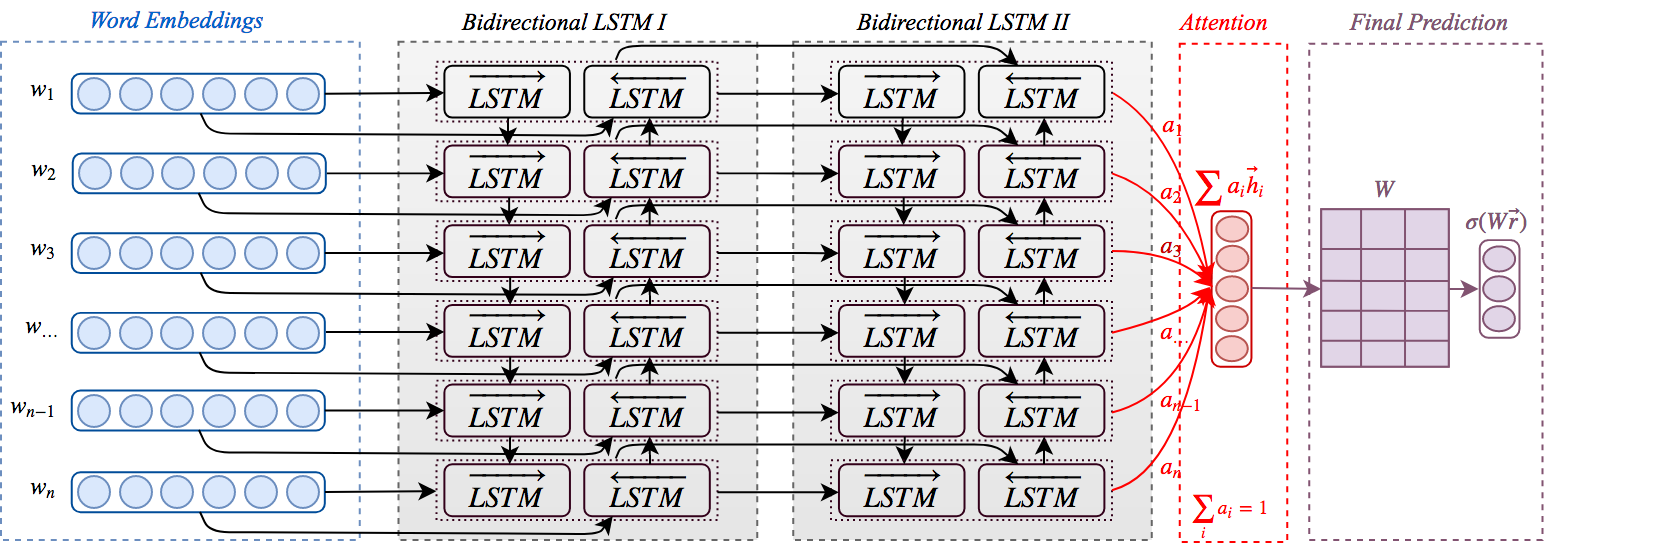
\includegraphics[width=\linewidth]{img/baziotis.png}
}
\caption[Neural network of \citet{Baziotis:17}]{Architecture of the
  neural network proposed
  by~\citet{Baziotis:17}}\label{cgsa:fig:baziotis}
\end{figure*}

Although the approach of~\citet{Baziotis:17} still represents the
current state of the art in sentiment analysis of Twitter and yields
extraordinarily good results, in our opinion, this method has yet some
potential for improvements.  This first of all concerns the way how
attention coefficients are computed.  As we can see from
Equation~\ref{eq:cgsa:baziotis-attention}, the magnitude of the
attention score $a_i$ primarily depends on the absolute value of the
LSTM outputs and the bias term at the $i$-th position.  Albeit this
strategy is plausible regarding the fact that polar terms that appear
at the end of a message usually have more impact on the net polarity
of the tweet than opinionated words that occur at the beginning, a
crucial prerequisite for this strategy to work is that
\begin{inparaenum}[(i)]
\item the LSTM layer already provides sufficiently reliable results
  and
\item the bias terms do not overly boost the importance of irrelevant
  tokens that just accidentally appeared at favored positions.
\end{inparaenum}
Unfortunately, both of these assumptions are rarely true, especially
when the training data are limited.

In order to overcome these drawbacks of position-based attention
scores, we decided to augment the original architecture
of~\citet{Baziotis:17} with two additional types of attention:
\emph{lexicon-} and \emph{context-based} one.  In the former of these
types, we estimated the importance weight $b_i$ for position $i$ using
the polarity score of the word $w_i$ from our linear projection
lexicon $V$, normalizing these scores over all positions $j$ from the
sequence:
\begin{align*}
  \vec{b} =& \sum_{i=1}^{|\mathbf{x}|}b_i\vec{h}_i,\\
  b_i =& \frac{\exp(f_i)}{\sum_{j=1}^{|\mathbf{x}|}\exp(f_j)},\textrm{ s.t.}\\
  f_i =& \left\{
  \begin{array}{ll}
    tanh(abs(V[{w_i}]) + \epsilon) & \textrm{ if } w_i\in V\\
    tanh(\epsilon) & \, \textrm{otherwise.} \\
  \end{array}
  \right .;
\end{align*}
\noindent In so doing, we hoped to force this layer to weigh the LSTM
outputs at subjective words more than its results at neutral tokens.

Even though polar terms definitely are one of the most influential
factors that affect message polarity, we should never forget that the
semantic orientation of these terms can easily be changed (and even
reversed) by various context factors \cite[see][]{Polanyi:06}.  To
account for this fact, we have introduced another type of
attention---the \emph{context-based} one, whose goal was to boost the
importance of elements which could act as potential valence shifters.
In order to identify such words, we applied another linear classifier
which predicted the potential shifting power of a token by looking at
the original embedding vector of this word and the LSTM output of its
parent in the dependency tree multiplied with the lexicon-based
attention score of the parent.  To keep the resulting values within an
appropriate range, we also used the same $tanh$ transformation and
global normalization over all positions as we did previously for the
position- and lexicon-based attentions:
\begin{align*}
  \vec{c} =& \sum_{i=1}^{|\mathbf{x}|}c_i\vec{h}_i,\\ c_i =&
  \frac{\exp(g_i)}{\sum_{j=1}^{|\mathbf{x}|}\exp(g_j)},\\ g_i =&
  \tanh\left(C [\vec{w}_i, \vec{b}_p]^\top\right);
\end{align*}
where $C\in\mathbb{R}^{200 \times 100}$ represents a context-based
attention matrix, $\vec{w}_i \in \mathbb{R}^{100}$ denotes the word
embedding of the $i$-th token, and $\vec{b}_p$ stands for the LSTM
output at the parent node of word $i$ times the lexicon-based
attention score of this node.  This way, we hoped to amplify the
importance of words like ``kaum'' (\textit{hardly}) or ``nicht''
(\textit{not}) in cases when the immediate syntactic ancestors of
these tokens were highly opinionated terms, e.g., ``Er hat die
Pr\"ufung kaum bestanden'' (\textit{He hardly passed the exam}) or
``Ich mag den neuen Bundesminister nicht'' (\textit{I do not like the
  new federal minister}).

Eventually, in order to make the final prediction, we concatenated the
outputs of the three attention layers into a single matrix
$A\in\mathbb{R}^{3 \times 100}$ and multiplied it with a vector
$\vec{w}\in\mathbb{R}^{1\times 100}$, applying softmax normalization
at the end:
\begin{align*}
  \vec{o} =& softmax\left(A^\top\vec{w}\right), \textrm{s.t.}\\
  A =& [\vec{a}, \vec{b}, \vec{c}].
\end{align*}

Since introducing additional attention types increased the number of
model parameters, we removed one of the Bi-LSTM layers to
counterbalance this effect and report our results for both settings:
with one and with two Bi-LSTM units (denoted as LBA$^{(1)}$ and
LBA$^{(2)}$ respectively).  The final architecture of our approach is
given in Figure~\ref{cgsa:fig:lba}.

% \done[inline]{\citet{Tang:14b}}

% A hybrid approach to coarse-grained sentiment analysis was proposed by
% \citet{Tang:14b}, who trained a linear SVM classifier on top of
% sentiment-specific word embeddings and hand-crafted features.  To
% obtain the former representations, \citeauthor{Tang:14b} devised a
% simple feed-forward neural network similar to the one used
% by~\citet{Collobert:11}, which, for each token $t$, had to predict the
% probability that this token appeared in the surrounding context and
% the likelihood that $t$ occurred in a positive or negative microblog.
% Since this training required a substantial amount of data, the authors
% leveraged a big collection of automatically downloaded tweets,
% obtaining noisy sentiment labels for these microblogs with the distant
% supervision method of~\citet{Go:09}.  The second part of this
% system---manually designed features---were mostly inspired by the work
% of~\citet{Mohammad:13} and included $n$-grams, word clusters,
% information about emoticons, negtaion, elongated characters and
% punctuation marks.  Combining these different traits into a single
% feature vector resulted significantly improved classification
% accuracy, yielding 0.701~\F{} on the SemEval-2014 test set (second
% place among all competing systems).

\begin{figure*}[htbp!]
{ \centering 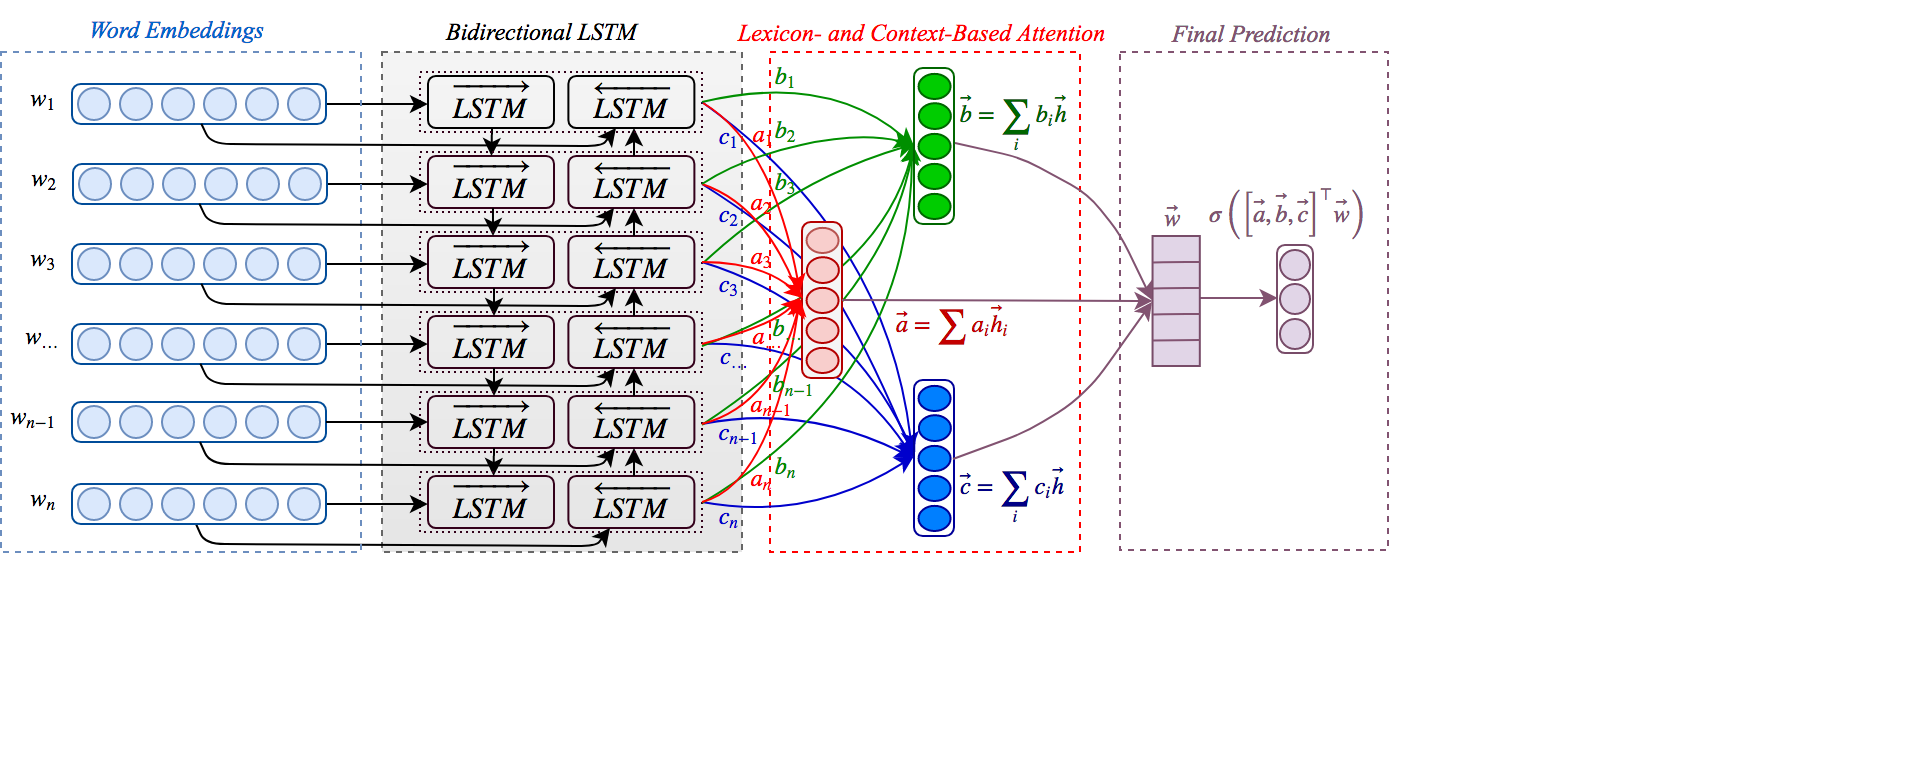
\includegraphics[width=1.3\linewidth]{img/lba.png} }
\caption[Neural network with lexicon-based attention]{Architecture of
  the neural network with lexicon- and context-based
  attention}\label{cgsa:fig:lba}
\end{figure*}


To evaluate the performance of the presented competitor methods and
also test our lexicon-based attention mechanism on the PotTS and SB10k
data, we have reimplemented the systems of~\citet{Yessenalina:11},
\citet{Socher:11,Socher:12,Socher:13}, \citet{Severyn:15},
and~\citet{Baziotis:17}, and applied them along with our own solution
to the aforementioned corpora.  For the sake of uniformity and
simplicity, we used task-specific word embeddings of
size~$\mathbb{R}^{100}$ in all of the systems, optimizing these
vectors with other network parameters during training.  Furthermore,
we also unified the final activation part and cost function of all
networks, using a densely connected softmax layer and optimizing the
weights w.r.t. the categorical hinge loss on the training data,
picking the values that yielded the highest accuracy on the validation
set.

\begin{table}[h]
  \begin{center}
    \bgroup \setlength\tabcolsep{0.1\tabcolsep}\scriptsize
    \begin{tabular}{p{0.162\columnwidth} % first columm
        *{9}{>{\centering\arraybackslash}p{0.074\columnwidth}} % next nine columns
        *{2}{>{\centering\arraybackslash}p{0.068\columnwidth}}} % last two columns
      \toprule
      \multirow{2}*{\bfseries Method} & %
      \multicolumn{3}{c}{\bfseries Positive} & %
      \multicolumn{3}{c}{\bfseries Negative} & %
      \multicolumn{3}{c}{\bfseries Neutral} & %
      \multirow{2}{0.068\columnwidth}{\bfseries\centering Macro\newline \F{}} & %
      \multirow{2}{0.068\columnwidth}{\bfseries\centering Micro\newline \F{}}\\
      \cmidrule(lr){2-4}\cmidrule(lr){5-7}\cmidrule(lr){8-10}

      & Precision & Recall & \F{} & %
      Precision & Recall & \F{} & %
      Precision & Recall & \F{} & & \\\midrule

      \multicolumn{12}{c}{\cellcolor{cellcolor}PotTS}\\

      %% Yessenalina Commands:
      %% -----------------
      %% cgsa_sentiment train -t yessenalina \
      %% data/PotTS/preprocessed/train/*.tsv data/PotTS/preprocessed/dev/*.tsv

      %% cgsa_sentiment test -m cgsa/data/models/cgsa.model data/PotTS/preprocessed/test/*.tsv\
      %% > data/PotTS/preprocessed/predicted/yessenalina/yessenalina.test

      %% cgsa_evaluate data/PotTS/preprocessed/test/ \
      %% data/PotTS/preprocessed/predicted/yessenalina/yessenalina.test

      %% General Statistics:
      %% precision    recall  f1-score   support
      %% positive       0.45      1.00      0.62       680
      %% negative       0.00      0.00      0.00       287
      %% neutral       0.00      0.00      0.00       558
      %% avg / total       0.20      0.45      0.28      1525
      %% Macro-Averaged F1-Score (Positive and Negative Classes): 30.84%
      %% Micro-Averaged F1-Score (All Classes): 44.5902%
      Y\&C & 0.45 & \textbf{1.0} & 0.62 & %
        0.0 & 0.0 & 0.0 & %
        0.0 & 0.0 & 0.0 & %
        0.308 & 0.446\\

        %% RAE Commands:
        %% -----------------
        %% cgsa_sentiment train -t rnn \
        %% data/PotTS/preprocessed/train/*.tsv data/PotTS/preprocessed/dev/*.tsv

        %% cgsa_sentiment test -m cgsa/data/models/cgsa.model data/PotTS/preprocessed/test/*.tsv\
        %% > data/PotTS/preprocessed/predicted/rnn/rnn.test

        %% cgsa_evaluate data/PotTS/preprocessed/test/ \
        %% data/PotTS/preprocessed/predicted/rnn/rnn.test

        %% RAE Results:
        %% ----------------
        %% General Statistics:
        %%              precision    recall  f1-score   support
        %%    positive       0.45      0.73      0.55       680
        %%    negative       0.24      0.01      0.03       287
        %%     neutral       0.35      0.25      0.29       558
        %% avg / total       0.37      0.42      0.36      1525
        %% Macro-Averaged F1-Score (Positive and Negative Classes): 28.97%
        %% Micro-Averaged F1-Score (All Classes): 41.7705%

      RAE & 0.45 & 0.73 & 0.55 & %
         0.24 & 0.01 & 0.03 & %
         0.35 & 0.25 & 0.29 & %
         0.29 & 0.418\\

         %% MVRNN Commands:
         %% -----------------
         %% cgsa_sentiment train -t mvrnn \
         %% data/PotTS/preprocessed/train/*.tsv data/PotTS/preprocessed/dev/*.tsv

         %% cgsa_sentiment test -m cgsa/data/models/cgsa.model data/PotTS/preprocessed/test/*.tsv\
         %% > data/PotTS/preprocessed/predicted/mvrnn/mvrnn.test

         %% cgsa_evaluate data/PotTS/preprocessed/test/ \
         %% data/PotTS/preprocessed/predicted/mvrnn/mvrnn.test

         %% MVRNN Results:
         %% ----------------
         %% General Statistics:
         %%              precision    recall  f1-score   support
         %%    positive       0.45      0.75      0.56       680
         %%    negative       0.22      0.03      0.06       287
         %%     neutral       0.38      0.25      0.30       558
         %% avg / total       0.38      0.43      0.37      1525
         %% Macro-Averaged F1-Score (Positive and Negative Classes): 31.19%
         %% Micro-Averaged F1-Score (All Classes): 42.9508%
      MVRNN & 0.45 & 0.75 & 0.56 & %
        0.22 & 0.03 & 0.06 & %
        0.38 & 0.25 & 0.3 & %
        0.312 & 0.43\\

        %% RNTN Commands:
        %% -----------------
        %% cgsa_sentiment train -t rntn \
        %% data/PotTS/preprocessed/train/*.tsv data/PotTS/preprocessed/dev/*.tsv

        %% cgsa_sentiment test -m cgsa/data/models/cgsa.model data/PotTS/preprocessed/test/*.tsv\
        %% > data/PotTS/preprocessed/predicted/rntn/rntn.test

        %% cgsa_evaluate data/PotTS/preprocessed/test/ \
        %% data/PotTS/preprocessed/predicted/rntn/rntn.test

        %% RNTN Results:
        %% ----------------
        %% General Statistics:
        %%              precision    recall  f1-score   support
        %%    positive       0.46      0.76      0.57       680
        %%    negative       0.18      0.11      0.13       287
        %%     neutral       0.37      0.15      0.22       558
        %% avg / total       0.37      0.41      0.36      1525
        %% Macro-Averaged F1-Score (Positive and Negative Classes): 35.25%
        %% Micro-Averaged F1-Score (All Classes): 41.3115%

       RNTN & 0.46 & 0.76 & 0.57 & %
         0.18 & 0.11 & 0.13 & %
         0.37 & 0.15 & 0.22 & %
         0.353 & 0.413\\

         %% Severyn Commands:
         %% -----------------
         %% cgsa_sentiment train -t severyn \
         %% data/PotTS/preprocessed/train/*.tsv data/PotTS/preprocessed/dev/*.tsv

         %% cgsa_sentiment test -m cgsa/data/models/cgsa.model data/PotTS/preprocessed/test/*.tsv\
         %% > data/PotTS/preprocessed/predicted/severyn/severyn.test

         %% cgsa_evaluate data/PotTS/preprocessed/test/ \
         %% data/PotTS/preprocessed/predicted/severyn/severyn.test

         %% Severyn Results:
         %% ----------------
         %% General Statistics:
         %%              precision    recall  f1-score   support
         %%    positive       0.71      0.78      0.74       680
         %%    negative       0.46      0.51      0.48       287
         %%     neutral       0.71      0.59      0.64       558
         %% avg / total       0.66      0.66      0.66      1525
         %% Macro-Averaged F1-Score (Positive and Negative Classes): 61.25%
         %% Micro-Averaged F1-Score (All Classes): 65.7705%

      SEV & 0.71 & 0.78 & 0.74 & %
         0.46 & \textbf{0.51} & \textbf{0.48} & %
         \textbf{0.71} & 0.59 & 0.64 & %
         \textbf{0.613} & 0.658\\

         %% Baziotis Commands:
         %% -----------------
         %% cgsa_sentiment train -t baziotis \
         %% data/PotTS/preprocessed/train/*.tsv data/PotTS/preprocessed/dev/*.tsv

         %% cgsa_sentiment test -m cgsa/data/models/cgsa.model data/PotTS/preprocessed/test/*.tsv\
         %% > data/PotTS/preprocessed/predicted/baziotis/baziotis.test

         %% cgsa_evaluate data/PotTS/preprocessed/test/ \
         %% data/PotTS/preprocessed/predicted/baziotis/baziotis.test

         %% Baziotis Results:
         %% ----------------
         %% General Statistics:
         %%              precision    recall  f1-score   support
         %%    positive       0.45      1.00      0.62       680
         %%    negative       0.00      0.00      0.00       287
         %%     neutral       0.00      0.00      0.00       558
         %% avg / total       0.20      0.45      0.28      1525
         %% Macro-Averaged F1-Score (Positive and Negative Classes): 30.84%
         %% Micro-Averaged F1-Score (All Classes): 44.5902%

         BAZ & 0.45 & \textbf{1.0} & 0.62 & %
         0.0 & 0.0 & 0.0 & %
         0.0 & 0.0 & 0.0 & %
         0.308 & 0.446\\

         % Lexicon-based Attention (1 BiLSTM) @b263b917dfe8755b10b9759f4ed0cecffa3534a1
         %% General Statistics:
         %% precision    recall  f1-score   support
         %% positive       0.81      0.73      0.77       680
         %% negative       0.60      0.15      0.24       287
         %% neutral       0.59      0.89      0.71       558
         %% avg / total       0.69      0.68      0.65      1525
         %% Macro-Averaged F1-Score (Positive and Negative Classes): 50.31%
         %% Micro-Averaged F1-Score (All Classes): 67.8033%
      LBA$^{(1)}$ & \textbf{0.81} & 0.73 & \textbf{0.77} & %
         \textbf{0.6} & 0.15 & 0.24 & %
         0.59 & \textbf{0.89} & \textbf{0.71} & %
         0.503 & \textbf{0.678}\\

         % Lexicon-based Attention (2 BiLSTM) @b263b917dfe8755b10b9759f4ed0cecffa3534a1
         %% General Statistics:
         %% precision    recall  f1-score   support
         %% positive       0.45      1.00      0.62       680
         %% negative       0.00      0.00      0.00       287
         %% neutral       0.00      0.00      0.00       558
         %% avg / total       0.20      0.45      0.28      1525
         %% Macro-Averaged F1-Score (Positive and Negative Classes): 30.84%
         %% Micro-Averaged F1-Score (All Classes): 44.5902%

         LBA$^{(2)}$ & 0.45 & \textbf{1.0} & 0.62 & %
         0.0 & 0.0 & 0.0 & %
         0.0 & 0.0 & 0.0 & %
         0.308 & 0.446\\

      \multicolumn{12}{c}{\cellcolor{cellcolor}SB10k}\\

      %% Yessenalina Commands:
      %% -----------------
      %% cgsa_sentiment train -t yessenalina \
      %% data/SB10k/preprocessed/train/*.tsv data/SB10k/preprocessed/dev/*.tsv

      %% cgsa_sentiment test -m cgsa/data/models/cgsa.model data/SB10k/preprocessed/test/*.tsv\
      %% > data/SB10k/preprocessed/predicted/yessenalina/yessenalina.test

      %% cgsa_evaluate data/SB10k/preprocessed/test/ \
      %% data/SB10k/preprocessed/predicted/yessenalina/yessenalina.test

      %% General Statistics:
      %% precision    recall  f1-score   support
      %% positive       0.00      0.00      0.00       354
      %% negative       0.00      0.00      0.00       212
      %% neutral       0.62      1.00      0.77       930

      %% avg / total       0.39      0.62      0.48      1496

      %% Macro-Averaged F1-Score (Positive and Negative Classes): 0.00%
      %% Micro-Averaged F1-Score (All Classes): 62.1658%

      Y\&C & 0.0 & 0.0 & 0.0 & %
        0.0 & 0.0 & 0.0 & %
        0.62 & \textbf{1.0} & 0.77 & %
        0.0 & 0.622\\

        %% RAE Commands:
        %% -------------
        %% cgsa_sentiment train -t rnn \
        %% data/SB10k/preprocessed/train/*.tsv data/SB10k/preprocessed/dev/*.tsv

        %% cgsa_sentiment test -m cgsa/data/models/cgsa.model data/SB10k/preprocessed/test/*.tsv\
        %% > data/SB10k/preprocessed/predicted/rnn/rnn.test

        %% cgsa_evaluate data/SB10k/preprocessed/test/ \
        %% data/SB10k/preprocessed/predicted/rnn/rnn.test

        %% RAE Results:
        %% ------------
        %% General Statistics:
        %%              precision    recall  f1-score   support
        %%    positive       0.20      0.09      0.12       354
        %%    negative       0.15      0.07      0.10       212
        %%     neutral       0.61      0.81      0.70       930
        %% avg / total       0.45      0.53      0.48      1496
        %% Macro-Averaged F1-Score (Positive and Negative Classes): 10.99%
        %% Micro-Averaged F1-Score (All Classes): 53.4091%

       RAE & 0.2 & 0.09 & 0.12 & %
         \textbf{0.15} & \textbf{0.07} & \textbf{0.1} & %
         0.61 & 0.81 & 0.7 & %
         0.101 & 0.534\\

         %% General Statistics:
         %%              precision    recall  f1-score   support
         %%    positive       0.50      0.01      0.01       354
         %%    negative       0.00      0.00      0.00       212
         %%     neutral       0.62      1.00      0.77       930
         %% avg / total       0.51      0.62      0.48      1496
         %% Macro-Averaged F1-Score (Positive and Negative Classes): 0.56%
         %% Micro-Averaged F1-Score (All Classes): 62.0989%

      MVRNN & 0.5 & 0.01 & 0.01 & %
        0.0 & 0.0 & 0.0 & %
        0.62 & \textbf{1.0} & 0.77 & %
        0.006 & 0.621\\

        %% General Statistics:
        %%              precision    recall  f1-score   support
        %%    positive       0.00      0.00      0.00       354
        %%    negative       0.00      0.00      0.00       212
        %%     neutral       0.62      1.00      0.77       930
        %% avg / total       0.39      0.62      0.48      1496
        %% Macro-Averaged F1-Score (Positive and Negative Classes): 0.00%
        %% Micro-Averaged F1-Score (All Classes): 62.1658%
      RNTN & 0.0 & 0.0 & 0.0 & %
        0.0 & 0.0 & 0.0 & %
        0.62 & \textbf{1.0} & 0.77 & %
        0.0 & 0.622\\

        % Severyn Commands:
        % -----------------
        % cgsa_sentiment train -t severyn \
        % data/SB10k/preprocessed/train/*.tsv data/SB10k/preprocessed/dev/*.tsv
        %
        % cgsa_sentiment test -m cgsa/data/models/cgsa.model data/SB10k/preprocessed/test/*.tsv\
        % > data/SB10k/preprocessed/predicted/severyn/severyn.test
        %
        % cgsa_evaluate data/SB10k/preprocessed/test/ \
        % data/SB10k/preprocessed/predicted/severyn/severyn.test
        %
        % Severyn Results:
        % ----------------
        %% General Statistics:
        %%              precision    recall  f1-score   support
        %%    positive       0.00      0.00      0.00       354
        %%    negative       0.00      0.00      0.00       212
        %%     neutral       0.62      1.00      0.77       930
        %% avg / total       0.39      0.62      0.48      1496
        %% Macro-Averaged F1-Score (Positive and Negative Classes): 0.00%
        %% Micro-Averaged F1-Score (All Classes): 62.1658%

       SEV & 0.0 & 0.0 & 0.0 & %
          0.0 & 0.0 & 0.0 & %
          0.62 & \textbf{1.0} & 0.77 & %
          0.0 & 0.622\\

          %% Baziotis Commands:
          %% -----------------
          %% cgsa_sentiment train -t baziotis \
          %% data/SB10k/preprocessed/train/*.tsv data/SB10k/preprocessed/dev/*.tsv

          %% cgsa_sentiment test -m cgsa/data/models/cgsa.model data/SB10k/preprocessed/test/*.tsv\
          %% > data/SB10k/preprocessed/predicted/baziotis/baziotis.test

          %% cgsa_evaluate data/SB10k/preprocessed/test/ \
          %% data/SB10k/preprocessed/predicted/baziotis/baziotis.test

          %% Baziotis Results:
          %% ----------------
          %% General Statistics:
          %% precision    recall  f1-score   support
          %% positive       0.65      0.60      0.62       354
          %% negative       0.00      0.00      0.00       212
          %% neutral       0.75      0.95      0.84       930
          %% avg / total       0.62      0.73      0.67      1496
          %% Macro-Averaged F1-Score (Positive and Negative Classes): 31.03%
          %% Micro-Averaged F1-Score (All Classes): 72.8610%
       BAZ & 0.66 & 0.6 & 0.62 & %
         0.0 & 0.0 & 0.0 & %
         0.75 & 0.95 & \textbf{0.84} & %
         0.31 & 0.729\\

         % Lexicon-based Attention (1 BiLSTM) @b263b917dfe8755b10b9759f4ed0cecffa3534a1
         %% General Statistics:
         %% General Statistics:
         %% precision    recall  f1-score   support
         %% positive       0.70      0.57      0.63       354
         %% negative       0.00      0.00      0.00       212
         %% neutral       0.74      0.97      0.84       930
         %% avg / total       0.63      0.74      0.67      1496
         %% Macro-Averaged F1-Score (Positive and Negative Classes): 31.41%
         %% Micro-Averaged F1-Score (All Classes): 73.5963%
       LBA$^{(1)}$ & \textbf{0.7} & 0.57 & \textbf{0.63} & %
        0.0 & 0.0 & 0.0 & %
        0.74 & 0.97 & \textbf{0.84} & %
        0.314 & \textbf{0.736}\\

        %% General Statistics:
        %% precision    recall  f1-score   support
        %% positive       0.63      0.63      0.63       354
        %% negative       0.00      0.00      0.00       212
        %% neutral       0.76      0.94      0.84       930
        %% avg / total       0.62      0.73      0.67      1496
        %% Macro-Averaged F1-Score (Positive and Negative Classes): 31.50%
        %% Micro-Averaged F1-Score (All Classes): 73.1283%

        LBA$^{(2)}$ & 0.63 & \textbf{0.63} & \textbf{0.63} & %
         0.0 & 0.0 & 0.0 & %
         \textbf{0.76} & 0.94 & \textbf{0.84} & %
         \textbf{0.315} & 0.731\\\bottomrule
    \end{tabular}
    \egroup
    \caption[Evaluation of DL-based CGSA methods]{ Evaluation of
      DL-based CGSA methods\\ {\small Y\&C~--~\citet{Yessenalina:11},
        RAE~--~Recursive Auto-Encoder \cite{Socher:11},
        MVRNN~--~Matrix-Vector RNN \cite{Socher:12}, RNTN~--~Recursive
        Neural-Tensor Network \cite{Socher:13},
        SEV~--~\citet{Severyn:15}, BAZ~--~\citet{Baziotis:17},
        LBA$^{(1)}$~--~lexicon-based attention with one Bi-LSTM
        layer, LBA$^{(2)}$~--~lexicon-based attention with two Bi-LSTM
        layers}}
    \label{snt-cgsa:tbl:dl-res}
  \end{center}
\end{table}

The results of this evaluation are shown in
Table~\ref{snt-cgsa:tbl:dl-res}.  As we can see from the figures, the
LBA method performs fairly well, especially for the positive and
neutral classes where it sets the best \F-benchmarks on both datasets
and consequently achieves the highest overall micro-averaged \F-scores
on all test samples (0.678 on PotTS and 0.736 on SB10k).  Even though
our approach also yields the best macro-averaged result on the SB10k
data~(0.315~\F), it seems to face a major difficulty with the extreme
label skewness of this corpus, failing to predict any negative tweet
on the provided test set.  This problem, in general, appears to be an
insurmountable hurdle for almost all other compared systems as well
and is especially aggravated for the matrix-space, RNTN, and
convolutional systems, all of which eventually always predict only the
most common neutral label and are unable to differentiate the other
two classes.  A single notable exception in this regard is the
recursive auto-encoder approach of~\citet{Socher:11}, which succeeds
in classifying some of the negative instances and also predicts the
positive and neutral labels, but whose precision and recall are still
far below an acceptable level.

A similar, though less severe situation is also observed with the
PotTS corpus.  This time, the Y\&C, BAZ, and LBA$^{(2)}$ methods lapse
into always predicting the most frequent polarity, which is positive
this time.  Other systems, however, perform much better, especially
the approach of~\citet{Severyn:15}, which does an extraordinarily good
job at classifying negative messages, reaching remarkable 0.48~\F for
this polarity and also attaining the best macro-average score (0.613)
on all tweets due to its even performance on positive and neutral
microblogs.  Nevertheless, even the best-performing DL systems (SEV
and LBA) lag far behind the traditional supervised machine-learning
method of~\citet{Mohammad:13}, and barely outperform the lexcon-based
approach of~\citet{Hu:04} in terms of the micro-averaged \F{} on
SB10k.  Two possible explanations for these rather mediocre results
that we can think of might be a bad starting point of the parameters,
which could prevent the optimizers from finding the optimal solution
to the optimization objective, or an insufficient amount of training
data, which would lead to an extreme overfitting of the training set,
but poor generalization to unseed examples.  We will now investigate
the former of these factors in detail.

% \section{Coarse-Grained Sentiment Analysis Using Language and Domain
%   Adaptation}\label{sec:cgsa:domain-adaptation}

% One of the first works which pointed out the importance of domain
% adaptation for sentiment analysis was introduced by~\citet{Aue:05}.
% In their experiments, the authors trained separate SVM classifiers on
% four different document sets: movie reviews, book reviews, customer
% feedback from a product support service, and a feedback survey from a
% customer knowledge base; finding that each classifier performed best
% when applied to the same domain as it was trained on.  In order to
% find an optimal way of overcoming this domain specificity,
% \citet{Aue:05} tried out four different options:
% \begin{inparaenum}[(i)]
% \item\label{sent-cgsa:lst:rel-wrk1} training one classifier on all but
%   the target domain and applying it to the latter;
% \item using the same procedure as above, but limiting the features to
%   only those which also appeared in the target texts;
% \item taking an ensemble of individual classifiers each of which was
%   trained on a different data collection; and, finally,
% \item using a minimal subset of labeled in-domain data to train a
%   Na{\"i}ve Bayes system with the expectation-maximization algorithm
%   \cite[EM;][]{Dempster:77}.
% \end{inparaenum}
% The authors found that the ensemble and EM options worked best for
% their cross-domain task, achieving an accuracy of up to 82.39\% for
% the two-class prediction (positive vs negative) on new unseen text
% genres.

% Another notable milestone in the domain adaptation research was set
% by~\citet{Blitzer:07}.  Relying on their previous work on structural
% correspondence learning~\cite{Blitzer:07}, in which they used a set of
% \emph{pivot features} (features which frequently appeared in both
% target and source domains) to find an optimal correspondence of the
% remaining attributes,\footnote{In particular, the authors trained $m$
%   binary predictors for each of their $m$ pivot features in order to
%   find other attributes which frequently co-occurred with the pivots.
%   Afterwards, they composed these $m$ resulting weight vectors into a
%   single matrix $W := [\vec{w}_{1},\ldots,\vec{w}_{m}]$, took an SVD
%   decomposition of this matrix, and used the top $h$ left singular
%   vectors to translate source features to the new domain.} the authors
% refined their method by pre-selecting the pivots using their PMI
% scores and improving misaligned feature projections using a small set
% of labeled target examples.  With these modifications,
% \citeauthor{Blitzer:07} were able to reduce the average adaptation
% loss (the accuracy drop when transferring a classifier to a different
% domain) from 9.1 to 4.9~percent when testing a sentiment predictor on
% the domains of book, dvd, electical appliances, and kitchen reviews.

% Other important works on domain adaptation for opinion mining include
% those of~\citet{Read:05}, who pointed out that sentiment
% classification might not only depend on the domain but also on topic,
% time, and language style in which the text was written;
% \citet{Tan:07}, who proposed using the classifier trained on the
% source domain to classify unlabeled instances from the target genre,
% and then iteratively retrain the system on the enriched data set.
% Finally, \citet{Andreevskaia:08} proposed a combination of a lexicon-
% and ML-based systems, claiming that this ensemble would be more
% resistible to the domain shift than each of these classifiers on their
% own.

% Another line of research was introduced by~\citet{Glorot:11} who
% proposed stacked denoising autoencoders (SDA)---a neural network
% architecture in which an input vector $\vec{x}$ was first mapped to a
% smaller representation $\vec{x}'$ via some function
% $h: \vec{x}\mapsto\vec{x}'$, and then restored to its approximate
% original state via an inverse transformation
% $g: \vec{x}'\mapsto\vec{x}''\approx\vec{x}$.  In their experiments,
% the authors optimized the parameters of the functions $h$ and $g$ on
% both target and source data, getting approximate representations of
% instances from both data sets; and then trained a linear SVM
% classifier on the restored representations of the source instances,
% subsequently applying this classifier to the target domain.  This
% approach was further refined by~\citet{Chen:12} who analytically
% computed the reconstruction function~$g$, and used both original and
% restored features to predict the polarity labels of the target
% data.\footnote{Both approaches were trained tested on the Amazon
%   Review Corpus of~\citet{Blitzer:07}.}


% Further notable contributions to domain adaptation in general were
% made by~\citet{Daume:07} who proposed to replicate each extracted
% feature three times and train the first replication on both domains,
% the second repetion only on source, and the third copy only on target
% domain, for which he assumed a small subset of labeled examples was
% available; \citet{Yang:15} who trained neural embeddings of features,
% trying to predict which instance attributes frequently co-occured with
% each other;

\subsection{Effect of Word Embeddings}

Similarly to what we did in the previous chapters, we decided to
replace the randomly initialized word vectors in the very first layer
of the neural networks with pre-trained word2vec embeddings, keeping
this parameter fixed during optimization.  As we can see from the
results in Table~\ref{snt-cgsa:tbl:dl-res-word2vec}, this operation
leads to a significant improvement of the results for all classifiers,
boosting the best observed macro-averaged \F-score from 0.613 to 0.651
on the PotTS corpus and increasing this value from 0.315 to 0.546 on
the SB10k data.  In a similar way, the accuracy of the models also
grows from 0.678 to 0.706 on the former dataset and from 0.736 to
0.759 on the \citeauthor{Cieliebak:17}'s corpus.

Another noteworthy tendency which we can observe after these changes
is that these improvements mostly affect models with a greater number
of intermediate paramaters, such as SEV, BAZ, LBA$^{(1)}$, and
LBA$^{(2)}$, but are significantly smaller for the recursive systems
(RAE and RNTN) which only have one compositional matrix or tensor to
unite the embeddings.

\begin{table}[h]
  \begin{center}
    \bgroup \setlength\tabcolsep{0.1\tabcolsep}\scriptsize
    \begin{tabular}{p{0.162\columnwidth} % first columm
        *{9}{>{\centering\arraybackslash}p{0.074\columnwidth}} % next nine columns
        *{2}{>{\centering\arraybackslash}p{0.068\columnwidth}}} % last two columns
      \toprule
      \multirow{2}*{\bfseries Method} & %
      \multicolumn{3}{c}{\bfseries Positive} & %
      \multicolumn{3}{c}{\bfseries Negative} & %
      \multicolumn{3}{c}{\bfseries Neutral} & %
      \multirow{2}{0.068\columnwidth}{\bfseries\centering Macro\newline \F{}} & %
      \multirow{2}{0.068\columnwidth}{\bfseries\centering Micro\newline \F{}}\\
      \cmidrule(lr){2-4}\cmidrule(lr){5-7}\cmidrule(lr){8-10}

      & Precision & Recall & \F{} & %
      Precision & Recall & \F{} & %
      Precision & Recall & \F{} & & \\\midrule

      \multicolumn{12}{c}{\cellcolor{cellcolor}PotTS}\\
         % Commands:
         % cgsa_sentiment train -t rnn --w2v data/PotTS/preprocessed/train/*.tsv \
         % data/PotTS/preprocessed/dev/*.tsv
         % cgsa_sentiment -v test data/PotTS/preprocessed/test/*.tsv > \
         % data/PotTS/preprocessed/predicted/rnn/rnn.word2vec.test
         % cgsa_evaluate data/PotTS/preprocessed/test/ \
         % data/PotTS/preprocessed/predicted/rnn/rnn.word2vec.test
      %% General Statistics:
      %% precision    recall  f1-score   support
      %% positive       0.45      0.96      0.61       680
      %% negative       0.33      0.00      0.01       287
      %% neutral       0.39      0.04      0.07       558

      %% avg / total       0.40      0.44      0.30      1525
      %% Macro-Averaged F1-Score (Positive and Negative Classes): 30.83%
      %% Micro-Averaged F1-Score (All Classes): 44.3934%

      RAE & 0.45 & \textbf{0.96} & 0.61 & %
          0.33 & 0.0 & 0.01 & %
          0.39 & 0.04 & 0.07 & %
          0.308 & 0.444\\

         % Commands:
         % cgsa_sentiment train -t rntn --w2v data/PotTS/preprocessed/train/*.tsv \
         % data/PotTS/preprocessed/dev/*.tsv
         % cgsa_sentiment -v test data/PotTS/preprocessed/test/*.tsv > \
         % data/PotTS/preprocessed/predicted/rntn/rntn.word2vec.test
         % cgsa_evaluate data/PotTS/preprocessed/test/ \
         % data/PotTS/preprocessed/predicted/rntn/rntn.word2vec.test
          %% General Statistics:
          %% precision    recall  f1-score   support
          %% positive       0.45      0.80      0.57       680
          %% negative       0.15      0.01      0.03       287
          %% neutral       0.39      0.20      0.26       558
          %% avg / total       0.37      0.43      0.36      1525
          %% Macro-Averaged F1-Score (Positive and Negative Classes): 29.82%
          %% Micro-Averaged F1-Score (All Classes): 42.9508%

      RNTN & 0.45 & 0.8 & 0.57 & %
          0.15 & 0.01 & 0.03 & %
          0.39 & 0.2 & 0.26 & %
          0.298 & 0.43\\

         % Commands:
         % cgsa_sentiment train -t severyn --w2v data/PotTS/preprocessed/train/*.tsv \
         % data/PotTS/preprocessed/dev/*.tsv
         % cgsa_sentiment -v test data/PotTS/preprocessed/test/*.tsv > \
         % data/PotTS/preprocessed/predicted/severyn/severyn.word2vec.test
         % cgsa_evaluate data/PotTS/preprocessed/test/ data/PotTS/preprocessed/predicted/severyn/severyn.word2vec.test
          %% General Statistics:
          %% precision    recall  f1-score   support
          %% positive       0.68      0.78      0.73       680
          %% negative       0.00      0.00      0.00       287
          %% neutral       0.61      0.82      0.70       558
          %% avg / total       0.53      0.65      0.58      1525
          %% Macro-Averaged F1-Score (Positive and Negative Classes): 36.41%
          %% Micro-Averaged F1-Score (All Classes): 64.7869%

      SEV & 0.68 & 0.78 & 0.73 & %
          0.0 & 0.0 & 0.0 & %
          0.61 & 0.82 & 0.7 & %
          0.364 & 0.648\\

         % Commands:
         % cgsa_sentiment train -t baziotis --w2v data/SB10k/preprocessed/train/*.tsv \
         % data/SB10k/preprocessed/dev/*.tsv
         % cgsa_sentiment -v test data/SB10k/preprocessed/test/*.tsv > \
         % data/SB10k/preprocessed/predicted/baziotis/baziotis.word2vec.test
         % cgsa_evaluate data/SB10k/preprocessed/test/ data/SB10k/preprocessed/predicted/baziotis/baziotis.word2vec.test
          %% General Statistics:
          %% precision    recall  f1-score   support
          %% positive       0.83      0.69      0.76       680
          %% negative       0.54      0.55      0.55       287
          %% neutral       0.67      0.80      0.73       558
          %% avg / total       0.72      0.71      0.71      1525
          %% Macro-Averaged F1-Score (Positive and Negative Classes): 65.09%
          %% Micro-Averaged F1-Score (All Classes): 70.5574%

      BAZ & 0.83 & 0.69 & \textbf{0.76} & %
          0.54 & \textbf{0.55} & 0.55 & %
          \textbf{0.67} & 0.8 & \textbf{0.73} & %
          \textbf{0.651} & \textbf{0.706}\\

          %% General Statistics:
          %% precision    recall  f1-score   support
          %% positive       0.85      0.64      0.73       680
          %% negative       0.56      0.55      0.56       287
          %% neutral       0.63      0.83      0.71       558
          %% avg / total       0.72      0.69      0.69      1525
          %% Macro-Averaged F1-Score (Positive and Negative Classes): 64.43%
          %% Micro-Averaged F1-Score (All Classes): 69.1803%

      LBA$^{(1)}$ & \textbf{0.85} & 0.64 & 0.73 & %
          0.56 & \textbf{0.55} & \textbf{0.56} & %
          0.63 & 0.83 & 0.71 & %
          0.644 & 0.692\\

          %% General Statistics:
          %% precision    recall  f1-score   support
          %% positive       0.84      0.62      0.71       680
          %% negative       0.65      0.26      0.37       287
          %% neutral       0.56      0.91      0.69       558
          %% avg / total       0.70      0.66      0.64      1525
          %% Macro-Averaged F1-Score (Positive and Negative Classes): 54.20%
          %% Micro-Averaged F1-Score (All Classes): 65.8361%

      LBA$^{(2)}$ & 0.84 & 0.62 & 0.71 & %
          \textbf{0.65} & 0.26 & 0.37 & %
          0.56 & \textbf{0.91} & 0.69 & %
          0.542 & 0.658\\

      \multicolumn{12}{c}{\cellcolor{cellcolor}SB10k}\\
         % Commands:
         % cgsa_sentiment train -t rnn --w2v data/SB10k/preprocessed/train/*.tsv \
         % data/SB10k/preprocessed/dev/*.tsv
         % cgsa_sentiment -v test data/SB10k/preprocessed/test/*.tsv > \
         % data/SB10k/preprocessed/predicted/rnn/rnn.word2vec.test
         % cgsa_evaluate data/SB10k/preprocessed/test/ \
         % data/SB10k/preprocessed/predicted/rnn/rnn.word2vec.test
      %% General Statistics:
      %% precision    recall  f1-score   support
      %% positive       0.27      0.07      0.11       354
      %% negative       0.10      0.02      0.04       212
      %% neutral       0.62      0.90      0.73       930
      %% avg / total       0.46      0.58      0.49      1496
      %% Macro-Averaged F1-Score (Positive and Negative Classes): 7.33%
      %% Micro-Averaged F1-Score (All Classes): 58.0214%

      RAE & 0.27 & 0.07 & 0.11 & %
          0.1 & 0.02 & 0.04 & %
          0.62 & 0.9 & 0.73 & %
          0.073 & 0.58\\

          %% General Statistics:
          %% precision    recall  f1-score   support
          %% positive       0.00      0.00      0.00       354
          %% negative       0.00      0.00      0.00       212
          %% neutral       0.62      1.00      0.77       930
          %% avg / total       0.39      0.62      0.48      1496
          %% Macro-Averaged F1-Score (Positive and Negative Classes): 0.00%
          %% Micro-Averaged F1-Score (All Classes): 62.1658%

      RNTN & 0.0 & 0.0 & 0.0 & %
         0.0 & 0.0 & 0.0 & %
         0.62 & \textbf{1.0} & 0.77 & %
         0.0 & 0.622\\

         % Commands:
         % cgsa_sentiment train -t severyn --w2v data/SB10k/preprocessed/train/*.tsv \
         % data/SB10k/preprocessed/dev/*.tsv
         % cgsa_sentiment -v test data/SB10k/preprocessed/test/*.tsv > \
         % data/SB10k/preprocessed/predicted/severyn/severyn.word2vec.test
         % cgsa_evaluate data/SB10k/preprocessed/test/ data/SB10k/preprocessed/predicted/severyn/severyn.word2vec.test
         %% General Statistics:
         %% precision    recall  f1-score   support
         %% positive       0.70      0.61      0.65       354
         %% negative       0.51      0.39      0.44       212
         %% neutral       0.80      0.88      0.83       930
         %% avg / total       0.73      0.74      0.73      1496
         %% Macro-Averaged F1-Score (Positive and Negative Classes): 54.56%
         %% Micro-Averaged F1-Score (All Classes): 74.3984%
      SEV & 0.7 & \textbf{0.61} & 0.65 & %
          0.51 & \textbf{0.39} & \textbf{0.44} & %
          \textbf{0.8} & 0.88 & 0.83 & %
          \textbf{0.546} & 0.744\\

         % Commands:
         % cgsa_sentiment train -t baziotis --w2v data/SB10k/preprocessed/train/*.tsv \
         % data/SB10k/preprocessed/dev/*.tsv
         % cgsa_sentiment -v test data/SB10k/preprocessed/test/*.tsv > \
         % data/SB10k/preprocessed/predicted/baziotis/baziotis.word2vec.test
         % cgsa_evaluate data/SB10k/preprocessed/test/ data/SB10k/preprocessed/predicted/baziotis/baziotis.word2vec.test
          %% General Statistics:
          %% precision    recall  f1-score   support
          %% positive       0.77      0.53      0.63       354
          %% negative       0.64      0.17      0.26       212
          %% neutral       0.74      0.96      0.84       930
          %% avg / total       0.74      0.75      0.71      1496
          %% Macro-Averaged F1-Score (Positive and Negative Classes): 44.60%
          %% Micro-Averaged F1-Score (All Classes): 74.5321%
      BAZ & \textbf{0.77} & 0.53 & 0.63 & %
          \textbf{0.64} & 0.17 & 0.26 & %
          0.74 & 0.96 & 0.84 & %
          0.446 & 0.745\\

          %% General Statistics:
          %% precision    recall  f1-score   support
          %% positive       0.75      0.60      0.67       354
          %% negative       0.59      0.22      0.32       212
          %% neutral       0.77      0.94      0.85       930
          %% avg / total       0.74      0.76      0.73      1496
          %% Macro-Averaged F1-Score (Positive and Negative Classes): 49.38%
          %% Micro-Averaged F1-Score (All Classes): 75.8690%
      LBA$^{(1)}$ & 0.75 & 0.6 & \textbf{0.67} & %
          0.59 & 0.22 & 0.32 & %
          0.77 & 0.94 & \textbf{0.85} & %
          0.494 & \textbf{0.759}\\

          %% General Statistics:
          %% precision    recall  f1-score   support
          %% positive       0.75      0.54      0.63       354
          %% negative       0.54      0.28      0.37       212
          %% neutral       0.76      0.93      0.84       930
          %% avg / total       0.73      0.75      0.72      1496
          %% Macro-Averaged F1-Score (Positive and Negative Classes): 50.04%
          %% Micro-Averaged F1-Score (All Classes): 74.5989%
      LBA$^{(2)}$ & 0.75 & 0.54 & 0.63 & %
          0.54 & 0.28 & 0.37 & %
          0.76 & 0.93 & 0.84 & %
          0.5 & 0.746\\\bottomrule

    \end{tabular}
    \egroup
    \caption[Evaluation of DL-based CGSA methods with pretrained
      word2vec vectors]{ Evaluation of DL-based CGSA methods with
      pretrained word2vec vectors\\ {\small RAE~--~Recursive
        Auto-Encoder \cite{Socher:11}, RNTN~--~Recursive Neural-Tensor
        Network \cite{Socher:13}, SEV~--~\citet{Severyn:15},
        BAZ~--~\citet{Baziotis:17}, LBA$^{(1)}$~--~lexicon-based
        attention with one Bi-LSTM layer, LBA$^{(2)}$~--~lexicon-based
        attention with two Bi-LSTM layers}}
    \label{snt-cgsa:tbl:dl-res-word2vec}
  \end{center}
\end{table}

In order to see whether this situation would be different if we
optimized word representations as well, we reran our experiments once
again, initializing word vectors with word2vec embeddings as
previously, but allowing them to be updated during the training.
Moreover, to account for words which were missing from the training
set, we additionally computed an optimal least-square mapping for
transforming original word2vec vectors to the best approximation of
optimized word represenations.  As suggested by the results in
Table~\ref{snt-cgsa:tbl:dl-res-lstsq}, these modifications iprove the
results even further, setting a new record for the macro-averaged
\F-value on the PotTS corpus (0.659~\F) and the micro-averaged
\F-score on the SB10k data (0.766~\F), and pushing our LBA$^{(1)}$
system even above its most challenging competitors.

\begin{table}[h]
  \begin{center}
    \bgroup \setlength\tabcolsep{0.1\tabcolsep}\scriptsize
    \begin{tabular}{p{0.162\columnwidth} % first columm
        *{9}{>{\centering\arraybackslash}p{0.074\columnwidth}} % next nine columns
        *{2}{>{\centering\arraybackslash}p{0.068\columnwidth}}} % last two columns
      \toprule
      \multirow{2}*{\bfseries Method} & %
      \multicolumn{3}{c}{\bfseries Positive} & %
      \multicolumn{3}{c}{\bfseries Negative} & %
      \multicolumn{3}{c}{\bfseries Neutral} & %
      \multirow{2}{0.068\columnwidth}{\bfseries\centering Macro\newline \F{}} & %
      \multirow{2}{0.068\columnwidth}{\bfseries\centering Micro\newline \F{}}\\
      \cmidrule(lr){2-4}\cmidrule(lr){5-7}\cmidrule(lr){8-10}

      & Precision & Recall & \F{} & %
      Precision & Recall & \F{} & %
      Precision & Recall & \F{} & & \\\midrule

      \multicolumn{12}{c}{\cellcolor{cellcolor}PotTS}\\
      %% General Statistics:
      %% precision    recall  f1-score   support
      %% positive       0.29      0.02      0.03       680
      %% negative       0.19      0.36      0.25       287
      %% neutral       0.37      0.61      0.46       558
      %% avg / total       0.30      0.30      0.23      1525
      %% Macro-Averaged F1-Score (Positive and Negative Classes): 13.91%
      %% Micro-Averaged F1-Score (All Classes): 29.9016%

      RAE & 0.29 & 0.02 & 0.03 & %
         0.19 & 0.36 & 0.25 & %
         0.37 & 0.61 & 0.46 & %
         0.139 & 0.299\\

         %% General Statistics:
         %% precision    recall  f1-score   support
         %% positive       0.41      0.44      0.42       680
         %% negative       0.15      0.13      0.14       287
         %% neutral       0.34      0.35      0.35       558
         %% avg / total       0.34      0.35      0.34      1525
         %% Macro-Averaged F1-Score (Positive and Negative Classes): 28.20%
         %% Micro-Averaged F1-Score (All Classes): 34.6230%

         RNTN & 0.41 & 0.44 & 0.42 & %
         0.15 & 0.13 & 0.14 & %
         0.34 & 0.35 & 0.35 & %
         0.282 & 0.346\\

         %% General Statistics:
         %% precision    recall  f1-score   support
         %% positive       0.71      0.78      0.74       680
         %% negative       0.00      0.00      0.00       287
         %% neutral       0.58      0.81      0.68       558
         %% avg / total       0.53      0.64      0.58      1525
         %% Macro-Averaged F1-Score (Positive and Negative Classes): 36.98%
         %% Micro-Averaged F1-Score (All Classes): 64.2623%

      SEV & 0.71 & 0.78 & 0.74 & %
         0.0 & 0.0 & 0.0 & %
         0.58 & 0.81 & 0.68 & %
         0.37 & 0.643\\

         %% General Statistics:
         %% precision    recall  f1-score   support
         %% positive       0.79      0.79      0.79       680
         %% negative       0.60      0.43      0.50       287
         %% neutral       0.68      0.79      0.73       558
         %% avg / total       0.71      0.72      0.71      1525
         %% Macro-Averaged F1-Score (Positive and Negative Classes): 64.28%
         %% Micro-Averaged F1-Score (All Classes): 71.8033%

         BAZ & 0.79 & 0.79 & \textbf{0.79} & %
         0.6 & 0.43 & 0.5 & %
         0.68 & 0.79 & \textbf{0.73} & %
         0.643 & \textbf{0.718}\\

         %% General Statistics:
         %% precision    recall  f1-score   support
         %% positive       0.71      0.85      0.77       680
         %% negative       0.64      0.48      0.55       287
         %% neutral       0.75      0.66      0.70       558
         %% avg / total       0.71      0.71      0.70      1525
         %% Macro-Averaged F1-Score (Positive and Negative Classes): 65.88%
         %% Micro-Averaged F1-Score (All Classes): 70.9508%
      LBA$^{(1)}$ & 0.71 & \textbf{0.85} & 0.77 & %
          \textbf{0.64} & \textbf{0.48} & \textbf{0.55} & %
          \textbf{0.75} & 0.66 & 0.7 & %
          \textbf{0.659} & 0.71\\

      %% General Statistics:
      %% precision    recall  f1-score   support
      %% positive       0.85      0.67      0.75       680
      %% negative       0.60      0.43      0.50       287
      %% neutral       0.62      0.86      0.72       558
      %% avg / total       0.72      0.70      0.69      1525
      %% Macro-Averaged F1-Score (Positive and Negative Classes): 62.58%
      %% Micro-Averaged F1-Score (All Classes): 69.5738%

      LBA$^{(2)}$ & \textbf{0.85} & 0.67 & 0.75 & %
          0.6 & 0.43 & 0.5 & %
          0.62 & \textbf{0.86} & 0.72 & %
          0.626 & 0.696\\

      \multicolumn{12}{c}{\cellcolor{cellcolor}SB10k}\\
      %% General Statistics:
      %%              precision    recall  f1-score   support
      %%    positive       0.30      0.26      0.28       354
      %%    negative       0.10      0.03      0.05       212
      %%     neutral       0.63      0.76      0.69       930
      %% avg / total       0.48      0.54      0.50      1496
      %% Macro-Averaged F1-Score (Positive and Negative Classes): 16.55%
      %% Micro-Averaged F1-Score (All Classes): 53.8770%

       RAE & 0.3 & 0.26 & 0.28 & %
         0.1 & 0.03 & 0.05 & %
         0.63 & 0.76 & 0.69 & %
         0.166 & 0.539\\

         %% General Statistics:
         %% precision    recall  f1-score   support
         %% positive       0.00      0.00      0.00       354
         %% negative       0.00      0.00      0.00       212
         %% neutral       0.62      1.00      0.77       930
         %% avg / total       0.39      0.62      0.48      1496
         %% Macro-Averaged F1-Score (Positive and Negative Classes): 0.00%
         %% Micro-Averaged F1-Score (All Classes): 62.0989%
      RNTN & 0.0 & 0.0 & 0.0 & %
        0.0 & 0.0 & 0.0 & %
        0.62 & \textbf{1.0} & 0.77 & %
        0.0 & 0.621\\

        %% General Statistics:
        %% precision    recall  f1-score   support
        %% positive       0.55      0.68      0.61       354
        %% negative       0.44      0.03      0.06       212
        %% neutral       0.78      0.87      0.82       930
        %% avg / total       0.68      0.71      0.66      1496
        %% Macro-Averaged F1-Score (Positive and Negative Classes): 33.41%
        %% Micro-Averaged F1-Score (All Classes): 70.7888%

      SEV & 0.55 & 0.68 & 0.61 & %
          0.44 & 0.03 & 0.06 & %
          0.78 & 0.87 & 0.82 & %
          0.334 & 0.708\\

          %% General Statistics:
          %% precision    recall  f1-score   support
          %% positive       0.69      0.64      0.67       354
          %% negative       0.57      0.30      0.39       212
          %% neutral       0.80      0.91      0.85       930
          %% avg / total       0.74      0.76      0.74      1496
          %% Macro-Averaged F1-Score (Positive and Negative Classes): 52.98%
          %% Micro-Averaged F1-Score (All Classes): 75.7353%

      BAZ & 0.69 & 0.64 & 0.67 & %
         0.57 & \textbf{0.3} & \textbf{0.39} & %
         \textbf{0.8} & 0.91 & \textbf{0.85} & %
         0.53 & 0.757\\

         %% General Statistics:
         %% precision    recall  f1-score   support
         %% positive       0.70      0.69      0.70       354
         %% negative       0.62      0.27      0.38       212
         %% neutral       0.80      0.91      0.85       930
         %% avg / total       0.75      0.77      0.75      1496
         %% Macro-Averaged F1-Score (Positive and Negative Classes): 53.90%
         %% Micro-Averaged F1-Score (All Classes): 76.6043%

      LBA$^{(1)}$ & 0.7 & \textbf{0.69} & \textbf{0.7} & %
          0.62 & 0.27 & 0.38 & %
          \textbf{0.8} & 0.91 & \textbf{0.85} & %
          \textbf{0.539} & \textbf{0.766}\\

      %% General Statistics:
      %% precision    recall  f1-score   support
      %% positive       0.79      0.50      0.61       354
      %% negative       0.63      0.18      0.28       212
      %% neutral       0.74      0.96      0.84       930
      %% avg / total       0.74      0.74      0.71      1496
      %% Macro-Averaged F1-Score (Positive and Negative Classes): 44.66%
      %% Micro-Averaged F1-Score (All Classes): 74.3984%

      LBA$^{(2)}$ & \textbf{0.79} & 0.5 & 0.61 & %
          \textbf{0.63} & 0.18 & 0.28 & %
          0.74 & 0.96 & 0.84 & %
          0.447 & 0.744\\\bottomrule
    \end{tabular}
    \egroup
    \caption[Evaluation of DL-based CGSA methods with pretrained least-squares embeddings]{
      Evaluation of DL-based CGSA methods with pretrained least-squares embeddings\\
      {\small RAE~--~Recursive
        Auto-Encoder \cite{Socher:11}, RNTN~--~Recursive Neural-Tensor Network
        \cite{Socher:13}, SEV~--~\citet{Severyn:15},
        BAZ~--~\citet{Baziotis:17}, , LBA$^{(1)}$~--~lexicon-based
        attention with one Bi-LSTM layer, LBA$^{(2)}$~--~lexicon-based
        attention with two Bi-LSTM layers}}
    \label{snt-cgsa:tbl:dl-res-lstsq}
  \end{center}
\end{table}

A similar effect is also observed for other systems, first of all BAZ
and LBA$^{(2)}$, which yield similarly good results for the positive
and neutral classes.  The only system which seems to be uaffected by
these improvements is the RNTN approach of~\citet{Socher:13}, which
keeps to predict the neutral label for all instances on the SB10k
corpus.

\subsection{Error Analysis}

Now, before we proceed with the evaluation of the other factor (a
larger size of the training set), let us first analyze some errors
that were specific to each classifier that was trained with
task-specific embeddings using the least-square fallback.

Since interpreting and understanding the results of deep learning
systems is a fairly complex problem in general due to a big number of
model parameters and unobvious correlations between them, we decided
to use \textsc{Lime}~\cite{Ribeiro:16}---a recently proposed local
interpretable model-agnostic explanation tool that can be used to
analyze the results of any black-box classifier.  To achieve this,
\textsc{Lime} randomly removes and perturbs parts of the input
instance and measures which of these modifications leads to the
biggest change of the output probabilities.

The first incorrect prediction shown in
Example~\ref{snt:cgsa:exmp:rae-error} was made by the recursive
auto-encoder system of~\citet{Socher:11}.  For the sake of vividness,
we highlighted all features that, according to \textsc{Lime}, are
associated with the neutral class as white, negative attributes are
marked with a \colorbox{blue!50}{blue} background, and positive
attributes are highlighted in \colorbox{green!50}{green}.  The
magnitude of color gradient shows the association strength of
particular feature with the respective class.

\begin{example}[Error Made by the RAE System]\label{snt:cgsa:exmp:rae-error}
  \noindent\textup{\bfseries\textcolor{darkred}{Tweet:}} {\upshape \colorbox{white!5}{Gr\"un}\colorbox{blue!11}{-}\colorbox{white!25.7}{Schwarz} \colorbox{white!5}{in} \colorbox{white!2.5!blue!1}{meinem} Bundesland. \colorbox{green!10}{Gef\"allt} \colorbox{white!5!blue!4.5}{mir} \colorbox{white!5!blue!5}{doch} \colorbox{white!4.6!blue!5}{sehr} \colorbox{white!5!blue!5}{\%PosSmiley}}\\
  \noindent \colorbox{white!5}{Green}\colorbox{blue!11}{-}\colorbox{white!25.7}{Black} \colorbox{white!5}{in} \colorbox{white!2.5!blue!1}{my} state.  \colorbox{white!5!blue!5}{Yet}, \colorbox{white!5!blue!4.5}{I} \colorbox{green!10}{like} it \colorbox{white!4.6!blue!5}{so much} \colorbox{white!5!blue!5}{\%PosSmiley}\\[\exampleSep]
  \noindent\textup{\bfseries\textcolor{darkred}{Gold Label:}}\hspace*{4.3em}\textbf{%
    \upshape\textcolor{green3}{positive}}\\
 \noindent\textup{\bfseries\textcolor{darkred}{Predicted Label:}}\hspace*{2em}\textbf{%
    \upshape\textcolor{black}{neutral*}}
\end{example}

%% <<<	gold:	neutral
%% >>>	predicted:	positive
%% 324606854040801280	Bundestagsdebatte : Von der Leyen schweigt beim Thema Frauenquote

%% <<<	gold:	neutral
%% >>>	predicted:	positive
%% 347465873210085379	Die vier apokalyptischen Reiter des Euro sind wieder gefragt ...

%% <<<	gold:	positive
%% >>>	predicted:	neutral
%% 370067678272430080	Wir lernen deutsch ! %PosSmiley

%% <<<	gold:	positive
%% >>>	predicted:	neutral
%% 371300430250516480	Sehr Gut %PosSmiley Leverkusen gewinnt Derby gegen Gladbach. nrw

%% <<<	gold:	positive
%% >>>	predicted:	neutral
%% 373555732970749953	Ach du scheisse ! %PosSmiley supercup BayernMunich

%% <<<	gold:	positive
%% >>>	predicted:	neutral
%% 390206322832314370	tztztztz .. %PosSmiley Spass !

%% <<<	gold:	positive
%% >>>	predicted:	neutral
%% 393338197133914112	Morgen lieve nichtje hier %PosSmiley

%% <<<	gold:	positive
%% >>>	predicted:	neutral
%% 394535574235004928	tumblr people sind meine lieblings people %PosSmiley

%% <<<	gold:	positive
%% >>>	predicted:	neutral
%% 395932235875905536	you ' re welcome %PosSmiley


\begin{example}[Error Made by the RNTN System]\label{snt:cgsa:exmp:socher13-error}
  \noindent\textup{\bfseries\textcolor{darkred}{Tweet: }} {\upshape
    tumblr people sind meine lieblings people \%PosSmiley}\\
  \noindent tumblr people are my favorite people \%PosSmiley\\[\exampleSep]
  \noindent\textup{\bfseries\textcolor{darkred}{Gold Label:}}\hspace*{4.3em}\textbf{%
    \upshape\textcolor{green3}{positive}}\\
 \noindent\textup{\bfseries\textcolor{darkred}{Predicted Label:}}\hspace*{2em}\textbf{%
    \upshape\textcolor{black}{neutral*}}
\end{example}

difficulties with possmiley

%% <<<	gold:	neutral
%% >>>	predicted:	positive
%% 311916228971229184	Ich muss schon wieder aufs Klo , aber sobald ich drauf sitze , kommt der Papst raus . Bestimmt .

%% <<<	gold:	negative
%% >>>	predicted:	neutral
%% 328110548975759360	Habe Hunger . Ihr seid mit Schuld . Als Deutsche sowieso .

%% <<<	gold:	negative
%% >>>	predicted:	neutral
%% 332278087922368512	Syrien ist Freund von Iran , das ist das Problem ! annewill

%% <<<	gold:	negative
%% >>>	predicted:	neutral
%% 362341966354198529	Otto Schily hat die SPD mit seinen �usserungen zum �berwachungsskandal in Schwierigkeiten gebracht . Was die NSA ...

%% <<<	gold:	negative
%% >>>	predicted:	neutral
%% 369706011709702144	Steuersenkungspl�ne : Trittin wirft der SPD �ngstlichkeit vor %Link �ngstlichkeit Steuersenkungspl�ne Trittin wirft

%% <<<	gold:	neutral
%% >>>	predicted:	negative
%% 368970863657246720	Achtung , Fanfare !

%% <<<	gold:	neutral
%% >>>	predicted:	positive
%% 370519824461340674	Achtung , fertig , los !

%% <<<	gold:	neutral
%% >>>	predicted:	positive
%% 391106605070422016	du f�rchtest wohl richtig

%% <<<	gold:	neutral
%% >>>	predicted:	negative
%% 393133078983741440	Schlauste idee Nicht

%% <<<	gold:	neutral
%% >>>	predicted:	negative
%% 393977627050250240	dunkel draussen ...

\begin{example}[Error Made by the SEV System]\label{snt:cgsa:exmp:severyn-error}
  \noindent\textup{\bfseries\textcolor{darkred}{Tweet:}} {\upshape }\\
  \noindent \\[\exampleSep]
  \noindent\textup{\bfseries\textcolor{darkred}{Gold Label:}}\hspace*{4.3em}\textbf{%
    \upshape\textcolor{green3}{positive}}\\
 \noindent\textup{\bfseries\textcolor{darkred}{Predicted Label:}}\hspace*{2em}\textbf{%
    \upshape\textcolor{black}{neutral*}}
\end{example}

%% <<<	gold:	neutral
%% >>>	predicted:	positive
%% 391697964189908992	Wollte meinen Kleiderschrank aufr�umen ... sitze nun darin und singe Liebeslieder ...

%% <<<	gold:	neutral
%% >>>	predicted:	negative
%% 376747161884446720	Ich muss diese Arbeitswoche �berleben ... f�r BTOB , BTS &amp; B. A. P

%% <<<	gold:	neutral
%% >>>	predicted:	positive
%% 391671355307208704	Verstehe . Gepanzerte Boote essen die Viecher , Stiefel lassen sie �brig , die schmecken nicht . Nat�rlich ! schlefaz

%% <<<	gold:	neutral
%% >>>	predicted:	positive
%% 373552746559188992	Die Bomben meiner Stadt machen BOOM , BOOM , BOOM !


\begin{example}[Error Made by the BAZ System]\label{snt:cgsa:exmp:baziotis-error}
  \noindent\textup{\bfseries\textcolor{darkred}{Tweet:}} {\upshape }\\
  \noindent \\[\exampleSep]
  \noindent\textup{\bfseries\textcolor{darkred}{Gold Label:}}\hspace*{4.3em}\textbf{%
    \upshape\textcolor{green3}{positive}}\\
 \noindent\textup{\bfseries\textcolor{darkred}{Predicted Label:}}\hspace*{2em}\textbf{%
    \upshape\textcolor{black}{neutral*}}
\end{example}

%% <<<	gold:	neutral
%% >>>	predicted:	negative
%% 322920577176334337	Zur Er�ffnung in Hannover wurde so viel geschrieben in Sachen Putin und die Razzien bei den deutschen Stiftungen ,

%% <<<	gold:	neutral
%% >>>	predicted:	positive
%% 367003093285601280	War das eine gute Idee ? - Amanda Bynes : Wiedersehen mit H�ndchen Sherbert : Sie hat ihn wieder ! Nachdem Amanda ...

%% <<<	gold:	neutral
%% >>>	predicted:	negative
%% 367922644089589760	Diesen Eindruck bekommt man momentan leider wirklich . Bin sowieso daf�r , dass H�bner die " 1 B " - L�sung forciert .


%% <<<	gold:	neutral
%% >>>	predicted:	positive
%% 370535615928238081	Bekommen Sie den besten Preis f\"ur Reich Hochzeitskleid Nicht z\"ogern ! ( nicht versp\"aten ) %Link fb

%% <<<	gold:	neutral
%% >>>	predicted:	negative
%% 370854706064941056	Omin�se Festplatte bestellt . Ohne grosse Ahnung , da ich keine sichere Auskunft des Auftraggebers bekam . %NegSmiley Breaking Bad S2 &amp; 3 mal dazugelegt .

%% <<<	gold:	neutral
%% >>>	predicted:	positive
%% 371687984086908928	Ach ja , damals %PosSmiley ( @ Mauerpark for Gr�ss August and Mutabor w / %User )

%% <<<	gold:	neutral
%% >>>	predicted:	positive
%% 371687984086908928	Ach ja , damals %PosSmiley ( @ Mauerpark for Gr�ss August and Mutabor w / %User )

%% <<<	gold:	neutral
%% >>>	predicted:	positive
%% 371910806411034624	Come on TeBe ! " 40. Minute : Hertha03 bisher ohne grosse Chancen . Die Abwehr steht gut . TeBeLive ...

%% <<<	gold:	neutral
%% >>>	predicted:	positive
%% 375739199405981696	Fliegen macht nicht in jede Richtung Spass .

%% <<<	gold:	neutral
%% >>>	predicted:	positive
%% 391701613066616832	bamba muss ein besseres stellungsspiel annehmen. klarer fehler beim 1-1 wenn zambrano rausr�ckt ...

%% <<<	gold:	neutral
%% >>>	predicted:	positive
%% 394406565803216896	Gerade super Lust , mit Carls Haaren was zu machen aber ca 300 km Distanz halten mich davon ab .

\begin{example}[Error Made by the LBA System]\label{snt:cgsa:exmp:lba-error}
  \noindent\textup{\bfseries\textcolor{darkred}{Tweet:}} {\upshape }\\
  \noindent \\[\exampleSep]
  \noindent\textup{\bfseries\textcolor{darkred}{Gold Label:}}\hspace*{4.3em}\textbf{%
    \upshape\textcolor{green3}{positive}}\\
 \noindent\textup{\bfseries\textcolor{darkred}{Predicted Label:}}\hspace*{2em}\textbf{%
    \upshape\textcolor{black}{neutral*}}
\end{example}

\section{Evaluation}
\subsection{Effect of Lexicons}\label{cgsa:subsec:eval:lexicons}

\todo[inline]{describe lexicon normalization steps}

\subsection{Effect of Distant Supervision}
\todo[inline]{}

To the best of our knowledge, the idea of utilizing web texts
containing emoticons as noisily labeled training data was first
proposed by~\citet{Read:05}, who collected a set of 26,000 Usenet
posts featuring smileys or frownies and used these documents to train
a Na{\"i}ve Bayes and SVM classifier.  The author demonstrated that,
despite some encouraging results obtained on the instances from the
same domain (up to 70\% accuracy), the trained systems did not
generalize well to other text genres, barely outperforming the chance
baseline and reaching a maximum accuracy of~54.4\% on news data and
56.8\% on movie reviews.

The presumably first known attempt to adopt distant supervision for
the sentiment analysis of Twitter data was made by~\citet{Go:09} who
collected a set of 800,000 positive and 800,000 negative microblogs
relying on emoticons as their noisy labels.  After stripping off these
smileys from text, the authors trained three independent
ML-classifiers (Na{\"i}ve Bayes, Maximum Entropy, and Support Vector
Machines) on this collection, achieving their best results (82.7\%
accuracy) with the NB and MaxEnt systems thaat utilized unigrams and
bigrams as features.

Another distantly supervised approach was presented
by~\citet{Barbosa:10}, who gathered a collection of automatically
labeled tweets from three popular sentiment web sites (Twendz, Twitter
Sentiment, and TweetFeel), and trained two binary SVM systems on this
corpus.  The first of these classifiers had to distinguish between
subjective and objective microblogs, attaining an error rate of~18.1\%
on a subset of 1,000 manually annotated messages.  In the next step,
the second system had to determine the semantic orientation of
opinionated posts (positive or negative), reaching an error rate
of~18.7\% on this prediction.

In a similar way, \citet{Pak:10} gathered a collection of 300,000
noisily labeled tweets, ensuring an even distribution of positive,
negative, and neutral messages.  After a brief exploration of PoS tag
statistics in these different classes, they presented a Na{\"i}ve
Bayes system which utilized highly relevant binary part-of-speech and
$n$-gram features.\footnote{\citet{Pak:10} determined the relevance of
  a feature $f$ using a special \emph{salience} metric, which was
  defined as a negative ratio between the minimum and maximum
  conditional probabilities of this feature belonging to different
  target classes:
  \begin{equation*}
    salience(f) = \frac{1}{N}\sum_{i=1}^{N-1}\sum_{j=i+1}^N 1 - \frac{\min(P(f, s_i), P(f, s_j))}{\max(P(f, s_i), P(f, s_j))},
  \end{equation*}
  where the $N$~term denotes the number of training examples, and
  $s_i$ means the sentiment class of the $i$-th training instance.}
With this approach, the authors attained an accuracy slighlty above
0.6 on the manually labeled test set of~\citet{Go:09}, also
demonstrating a particular utility of bigrams, negation rules, and
feature pruning heuristics.

A slightly different task was addressed by~\citet{Davidov:10}, who
sought to predict hashtags and emoticons occurring in tweets using a
$k$-NN classifier trained on a large collection of messages.  The
authors achieved an \F-measure of~0.31 on the former task, and reached
an \F-score of~0.64 on predicting smileys.

\citet{Kouloumpis:11} trained an AdaBoost
classifier~\cite{Schapire:00} on two large collections of noisily
labeled tweets---the emoticon tweebank of~\citet{Go:09} and the
Edinburgh hashtag corpus.\footnote{\url{http://demeter.inf.ed.ac.uk}}
Using $n$-gram (up to length two), lexicon, part-of-speech, and
micro-blogging features (such as emoticons, abbreviations, and slang
expressions), the authors achieved a macro-averaged \F-measure of~0.68
on the three-class prediction task.

\subsection{Effect of Text Normalization}
\begin{table}[h]
  \begin{center}
    \bgroup \setlength\tabcolsep{0.1\tabcolsep}\scriptsize
    \begin{tabular}{p{0.162\columnwidth} % first columm
        *{9}{>{\centering\arraybackslash}p{0.074\columnwidth}} % next nine columns
        *{2}{>{\centering\arraybackslash}p{0.068\columnwidth}}} % last two columns
      \toprule
      \multirow{2}*{\bfseries Method} & %
      \multicolumn{3}{c}{\bfseries Positive} & %
      \multicolumn{3}{c}{\bfseries Negative} & %
      \multicolumn{3}{c}{\bfseries Neutral} & %
      \multirow{2}{0.068\columnwidth}{\bfseries\centering Macro\newline \F{}$^{+/-}$} & %
      \multirow{2}{0.068\columnwidth}{\bfseries\centering Micro\newline \F{}}\\
      \cmidrule(lr){2-4}\cmidrule(lr){5-7}\cmidrule(lr){8-10}

      & Precision & Recall & \F{} & %
      Precision & Recall & \F{} & %
      Precision & Recall & \F{} & & \\\midrule

      \multicolumn{12}{c}{\cellcolor{cellcolor}PotTS}\\

      % Training hu-liu
      % Testing hu-liu
      % Evaluating hu-liu
      % General Statistics:
      % precision    recall  f1-score   support
      % positive       0.63      0.30      0.40       691
      % negative       0.46      0.29      0.36       296
      % neutral       0.41      0.77      0.54       542
      % avg / total       0.52      0.46      0.44      1529
      % Macro-Averaged F1-Score (Positive and Negative Classes): 38.00%
      % Micro-Averaged F1-Score (All Classes): 46.4356%
      HL & 0.63 & 0.3 & 0.4 & %
        0.46 & 0.29 & 0.36 & %
        0.41 & 0.77 & 0.54 & %
        0.38 & 0.464\\

        % Training taboada
        % Testing taboada
        % Evaluating taboada
        % General Statistics:
        % precision    recall  f1-score   support
        % positive       0.65      0.24      0.36       691
        % negative       0.46      0.27      0.34       296
        % neutral       0.41      0.83      0.55       542
        % avg / total       0.53      0.46      0.42      1529
        % Macro-Averaged F1-Score (Positive and Negative Classes): 34.81%
        % Micro-Averaged F1-Score (All Classes): 45.6508%

      TBD & 0.65 & 0.24 & 0.36 & %
        0.46 & 0.27 & 0.34 & %
        0.41 & 0.83 & 0.55 & %
        0.348 & 0.457\\

        % Training musto
        % Testing musto
        % Evaluating musto
        % General Statistics:
        % precision    recall  f1-score   support
        % positive       0.63      0.29      0.40       691
        % negative       0.47      0.34      0.39       296
        % neutral       0.42      0.77      0.54       542
        % avg / total       0.52      0.47      0.45      1529
        % Macro-Averaged F1-Score (Positive and Negative Classes): 39.47%
        % Micro-Averaged F1-Score (All Classes): 46.9588%
      MST & 0.63 & 0.29 & 0.4 & %
        0.47 & 0.34 & 0.39 & %
        0.42 & 0.77 & 0.54 & %
        0.395 & 0.47\\

        % Training jurek
        % Testing jurek
        % Evaluating jurek
        % General Statistics:
        % precision    recall  f1-score   support
        % positive       0.59      0.30      0.40       691
        % negative       0.42      0.18      0.25       296
        % neutral       0.41      0.80      0.54       542
        % avg / total       0.50      0.45      0.42      1529
        % Macro-Averaged F1-Score (Positive and Negative Classes): 32.69%
        % Micro-Averaged F1-Score (All Classes): 45.3891%
      JRK & 0.44 & 0.22 & 0.29 & %
        0.14 & 0.06 & 0.08 & %
        0.36 & 0.7 & 0.47 & %
        0.189 & 0.359\\

        % Training kolchyna
        % Testing kolchyna
        % Evaluating kolchyna
        % General Statistics:
        % precision    recall  f1-score   support
        % positive       0.61      0.23      0.33       691
        % negative       0.33      0.21      0.26       296
        % neutral       0.41      0.82      0.55       542
        % avg / total       0.48      0.43      0.39      1529
        % Macro-Averaged F1-Score (Positive and Negative Classes): 29.52%
        % Micro-Averaged F1-Score (All Classes): 43.4925%
      KLCH & 0.61 & 0.23 & 0.33 & %
        0.33 & 0.21 & 0.26 & %
        0.41 & 0.82 & 0.55 & %
        0.295 & 0.435 \\

      \multicolumn{12}{c}{\cellcolor{cellcolor}SB10k}\\

      % Training hu-liu
      % Testing hu-liu
      % Evaluating hu-liu
      % General Statistics:
      % precision    recall  f1-score   support
      % positive       0.41      0.42      0.42       354
      % negative       0.24      0.28      0.26       212
      % neutral       0.66      0.63      0.65       930
      % avg / total       0.54      0.53      0.54      1496
      % Macro-Averaged F1-Score (Positive and Negative Classes): 33.75%
      % Micro-Averaged F1-Score (All Classes): 53.2086%
      HL & 0.41 & 0.42 & 0.42 & %
        0.24 & 0.28 & 0.26 & %
        0.66 & 0.63 & 0.65 & %
        0.338 & 0.532\\

        % Training taboada
        % Testing taboada
        % Evaluating taboada
        % General Statistics:
        % precision    recall  f1-score   support
        % positive       0.41      0.37      0.39       354
        % negative       0.21      0.24      0.22       212
        % neutral       0.65      0.66      0.66       930
        % avg / total       0.53      0.53      0.53      1496
        % Macro-Averaged F1-Score (Positive and Negative Classes): 30.77%
        % Micro-Averaged F1-Score (All Classes): 53.3422%
      TBD & 0.41 & 0.37 & 0.39 & %
        0.21 & 0.24 & 0.22 & %
        0.65 & 0.66 & 0.66 & %
        0.308 & 0.533\\

        % Training musto
        % Testing musto
        % Evaluating musto
        % General Statistics:
        % precision    recall  f1-score   support
        % positive       0.40      0.32      0.35       354
        % negative       0.26      0.30      0.28       212
        % neutral       0.65      0.68      0.67       930
        % avg / total       0.54      0.54      0.54      1496
        % Macro-Averaged F1-Score (Positive and Negative Classes): 31.55%
        % Micro-Averaged F1-Score (All Classes): 54.0775%
      MST & 0.4 & 0.32 & 0.35 & %
        0.26 & 0.3 & 0.28 & %
        0.65 & 0.68 & 0.67 & %
        0.316 & 0.541\\

        % Training jurek
        % Testing jurek
        % Evaluating jurek
        % General Statistics:
        % precision    recall  f1-score   support
        % positive       0.40      0.42      0.41       354
        % negative       0.36      0.26      0.30       212
        % neutral       0.69      0.72      0.71       930
        % avg / total       0.58      0.59      0.58      1496
        % Macro-Averaged F1-Score (Positive and Negative Classes): 35.67%
        % Micro-Averaged F1-Score (All Classes): 58.5561%
      JRK & 0.4 & 0.42 & 0.41 & %
        0.36 & 0.26 & 0.3 & %
        0.69 & 0.72 & 0.71 & %
        0.357 & 0.586\\

        % Training kolchyna
        % Testing kolchyna
        % Evaluating kolchyna
        % General Statistics:
        % precision    recall  f1-score   support
        % positive       0.42      0.21      0.28       354
        % negative       0.25      0.13      0.17       212
        % neutral       0.66      0.86      0.75       930
        % avg / total       0.55      0.60      0.56      1496
        % Macro-Averaged F1-Score (Positive and Negative Classes): 22.51%
        % Micro-Averaged F1-Score (All Classes): 60.3610%
      KLCH & 0.42 & 0.21 & 0.28 & %
       0.25 & 0.13 & 0.17 & %
       0.66 & 0.86 & 0.75 & %
       0.225 & 0.604\\\bottomrule
\end{tabular}
    \egroup
    \caption[Results of CGSA Methods without Text Normalization]{
      Results of CGSA methods without text normalization\\
      {\small HL~--~\citet{Hu:04}, TBD~--~\citet{Taboada:11}, MST~-- \citet{Musto:14}, JRK
        -- \citet{Jurek:15}, KLCH -- \citet{Kolchyna:15}}}
    \label{snt-cgsa:tbl:res-without-normalization}
  \end{center}
\end{table}

\section{Summary and Conclusions}\label{slsa:subsec:conclusions}
